\documentclass[12pt]{book}

\usepackage[top=1in, bottom=1in, left=1.5in, right=1.5in, letterpaper]{geometry}
\usepackage{booktabs}
\usepackage{setspace}
\usepackage{trackchanges}
\usepackage{fancyhdr}
\usepackage{etoolbox}
\usepackage{lipsum}
\usepackage{amsmath}
\usepackage{listings}
\usepackage{wasysym}
\usepackage{float}
\usepackage[font=small,labelfont=bf]{caption}
\usepackage[caption=false,font=footnotesize,format=hang]{subfig}
\usepackage{pgfplots}
\pgfplotsset{compat=newest}
\usepackage{pgfplotstable}
\usetikzlibrary{plotmarks,arrows}
\tikzset{>=latex}
%\usepgfplotslibrary{colorbrewer}
\usepackage[absolute,overlay]{textpos}
\usepackage{graphicx}
\usepackage{lmodern}
\usepackage{longtable}
\usepackage{xfrac}
\usepackage{siunitx}
\usepackage[style=ieee,backend=biber]{biblatex}
\addbibresource{references.bib}
\usepackage[hidelinks, bookmarks=true]{hyperref}
\usepackage{bookmark}
\usepackage{algorithmicx}
\usepackage{algpseudocode}
\usepackage[chapter]{algorithm}
%\usepackage{droid}
\usepackage[T1]{fontenc}
\usepackage[titletoc]{appendix}
\usepackage[section]{placeins}
\usepackage{xparse}
\usepackage{etoolbox}
\usepackage{ifthen}
\usepackage{multicol}

% add a "DRAFT" watermark to everything
%\usepackage{draftwatermark}
%\SetWatermarkLightness{0.8}
%\SetWatermarkScale{1.5}

% set up SIunitsX
\sisetup{
	group-four-digits = true,
	group-separator = {,},
	%per=frac,
	%fraction=nice
	%fraction=sfrac
	%per-mode=symbol,
	list-separator = {, },
	list-final-separator = {, },
}
%\newcommand{\usd}[1]{\SI{#1}[\$\ensuremath{\,}]{}}
\newcommand{\percent}{\%}

% set up colours for plots
% these are based on mapping colours that should photocopy in black and white well

\definecolor{pc1}{HTML}{8DD3C7}
\definecolor{pc2}{HTML}{FDB462}
\definecolor{pc3}{HTML}{FB8072}
\definecolor{pc4}{HTML}{80B1D3}
\definecolor{pc5}{HTML}{B3DE69}
\definecolor{pc6}{HTML}{BEBADA}
\definecolor{pc7}{HTML}{FCCDE5}
\definecolor{pc8}{HTML}{D9D9D9}
\definecolor{pc9}{HTML}{FFFFB3}

%\definecolor{pc1}{HTML}{8DD3C7}
%\definecolor{pc2}{HTML}{FFFFB3}
%\definecolor{pc3}{HTML}{BEBADA}
%\definecolor{pc4}{HTML}{FB8072}
%\definecolor{pc5}{HTML}{80B1D3}
%\definecolor{pc6}{HTML}{FDB462}
%\definecolor{pc7}{HTML}{B3DE69}
%\definecolor{pc8}{HTML}{FCCDE5}
%\definecolor{pc9}{HTML}{D9D9D9}

%\pgfplotscreateplotcyclelist{ColourPlotCycle}{%
%solid,ultra thick,pc1,every mark/.append style={fill=pc1},mark=*\\%
%solid,ultra thick,pc2,every mark/.append style={fill=pc2},mark=square*\\%
%solid,ultra thick,pc3,every mark/.append style={fill=pc3},mark=diamond*\\%
%solid,ultra thick,pc4,every mark/.append style={fill=pc4},mark=pentagon*\\%
%solid,ultra thick,pc5,every mark/.append style={fill=pc5},mark=triangle*\\%
%dashed,ultra thick,pc6,every mark/.append style={fill=pc6},mark=*\\%
%dashed,ultra thick,pc7,every mark/.append style={fill=pc7},mark=square*\\%
%dashed,ultra thick,pc8,every mark/.append style={fill=pc8},mark=diamond*\\%
%dashed,ultra thick,pc9,every mark/.append style={fill=pc9},mark=pentagon*\\%
%}
\pgfplotscreateplotcyclelist{ColourPlotCycle}{%
only marks,solid,ultra thick,pc1,every mark/.append style={fill=pc1},mark=o\\%
only marks,dashed,ultra thick,pc2,every mark/.append style={fill=pc2},mark=square\\%
only marks,dotted,ultra thick,pc3,every mark/.append style={fill=pc3},mark=diamond*\\%
only marks,dashdotted,ultra thick,pc4,every mark/.append style={fill=pc4},mark=pentagon*\\%
only marks,solid,ultra thick,pc5,every mark/.append style={fill=pc5},mark=triangle*\\%
only marks,dashed,ultra thick,pc6,every mark/.append style={fill=pc6},mark=*\\%
only marks,dotted,ultra thick,pc7,every mark/.append style={fill=pc7},mark=square*\\%
only marks,dashdotted,ultra thick,pc8,every mark/.append style={fill=pc8},mark=diamond\\%
only marks,solid,ultra thick,pc9,every mark/.append style={fill=pc9},mark=pentagon\\%
}
\pgfplotscreateplotcyclelist{ColourPlotRegressionCycle}{%
only marks,solid,ultra thick,pc1,every mark/.append style={fill=pc1},mark=o\\%
solid,ultra thick,pc1\\%
only marks,dashed,ultra thick,pc2,every mark/.append style={fill=pc2},mark=square\\%
dashed,ultra thick,pc2\\%
only marks,dotted,ultra thick,pc3,every mark/.append style={fill=pc3},mark=diamond*\\%
dotted,ultra thick,pc3\\%
only marks,dashdotted,ultra thick,pc4,every mark/.append style={fill=pc4},mark=pentagon*\\%
dashdotted,ultra thick,pc4\\%
only marks,solid,ultra thick,pc5,every mark/.append style={fill=pc5},mark=triangle*\\%
solid,ultra thick,pc5\\%
only marks,dashed,ultra thick,pc6,every mark/.append style={fill=pc6},mark=*\\%
dashed,ultra thick,pc6\\%
only marks,dotted,ultra thick,pc7,every mark/.append style={fill=pc7},mark=square*\\%
dotted,ultra thick,pc7\\%
only marks,dashdotted,ultra thick,pc8,every mark/.append style={fill=pc8},mark=diamond\\%
dashdotted,ultra thick,pc8\\%
only marks,solid,ultra thick,pc9,every mark/.append style={fill=pc9},mark=pentagon\\%
solid,ultra thick,pc9\\%
}
\pgfplotscreateplotcyclelist{SmoothColourPlotCycle}{%
solid,ultra thick,pc1\\%
dashed,ultra thick,pc2\\%
dotted,ultra thick,pc3\\%
dashdotted,ultra thick,pc4\\%
solid,ultra thick,pc5\\%
dashed,ultra thick,pc6\\%
dotted,ultra thick,pc7\\%
dashdotted,ultra thick,pc8\\%
solid,ultra thick,pc9\\%
}
\pgfplotscreateplotcyclelist{BarColourPlotCycle}{%
fill=pc1\\%
fill=pc2\\%
fill=pc3\\%
fill=pc4\\%
fill=pc5\\%
fill=pc6\\%
fill=pc7\\%
fill=pc8\\%
fill=pc9\\%
}

\definecolor{RdBuWhiteGrey}{RGB}{247,247,247}
\pgfplotsset{
	colormap={RdBu}{
		rgb255(0cm)=(5,48,97);
		rgb255(1cm)=(33,102,172);
		rgb255(2cm)=(67,147,195);
		rgb255(3cm)=(146,197,222);
		rgb255(4cm)=(209,229,240);
		rgb255(5cm)=(247,247,247);
		rgb255(6cm)=(253,219,199);
		rgb255(7cm)=(244,165,130);
		rgb255(8cm)=(214,96,77);
		rgb255(9cm)=(178,24,43);
		rgb255(10cm)=(103,0,31);
	}
}
\pgfplotsset{
	colormap={YlOrRd}{
		rgb255(0cm)=(128,0,38);
		rgb255(1cm)=(189,0,38);
		rgb255(2cm)=(227,26,28);
		rgb255(3cm)=(252,78,42);
		rgb255(4cm)=(253,141,60);
		rgb255(5cm)=(254,178,76);
		rgb255(6cm)=(254,217,118);
		rgb255(7cm)=(255,237,160);
		rgb255(8cm)=(255,255,204);
	}
}

% for drawing legends with regressions
\newcommand{\drawLegendMarks}[1]{
	\addlegendimage{empty legend}
	\addlegendimage{solid,ultra thick,pc1,every mark/.append style={fill=pc1},mark=o}
	\ifnum#1>1
		\addlegendimage{dashed,ultra thick,pc2,every mark/.append style={fill=pc2},mark=square}
	\fi
	\ifnum#1>2
		\addlegendimage{dotted,ultra thick,pc3,every mark/.append style={fill=pc3},mark=diamond*}
	\fi
	\ifnum#1>3
		\addlegendimage{dashdotted,ultra thick,pc4,every mark/.append style={fill=pc4},mark=pentagon*}
	\fi
	\ifnum#1>4
		\addlegendimage{solid,ultra thick,pc5,every mark/.append style={fill=pc5},mark=triangle*}
	\fi
	\ifnum#1>5
		\addlegendimage{dashed,ultra thick,pc6,every mark/.append style={fill=pc6},mark=*}
	\fi
	\ifnum#1>6
		\addlegendimage{dotted,ultra thick,pc7,every mark/.append style={fill=pc7},mark=square*}
	\fi
	\ifnum#1>7
		\addlegendimage{dashdotted,ultra thick,pc8,every mark/.append style={fill=pc8},mark=diamond}
	\fi
	\ifnum#1>8
		\addlegendimage{solid,ultra thick,pc9,every mark/.append style={fill=pc9},mark=pentagon}
	\fi
}

\DeclareDocumentCommand\characterizationPlots{ m m g g g g }{%
	\addplot+[forget plot] table{assets/#2}; \pgfplotsset{cycle list shift=1};%
	\addplot+[forget plot] table[y={create col/linear regression={y=#1}}] {assets/#2}; \pgfplotsset{cycle list shift=2};%
	\xdef\slopeA{\pgfplotstableregressiona}; \xdef\interA{\pgfplotstableregressionb};%
	\IfNoValueF {#3} {%
		\addplot+[forget plot] table{assets/#3}; \pgfplotsset{cycle list shift=3};%
		\addplot+[forget plot] table[y={create col/linear regression={y=#1}}] {assets/#3}; \pgfplotsset{cycle list shift=4};%
		\xdef\slopeB{\pgfplotstableregressiona}; \xdef\interB{\pgfplotstableregressionb};%
	}%
	\IfNoValueF {#4} {%
		\addplot+[forget plot] table{assets/#4}; \pgfplotsset{cycle list shift=5};%
		\addplot+[forget plot] table[y={create col/linear regression={y=#1}}] {assets/#4}; \pgfplotsset{cycle list shift=6};%
		\xdef\slopeC{\pgfplotstableregressiona}; \xdef\interC{\pgfplotstableregressionb};%
	}%
	\IfNoValueF {#5} {%
		\addplot+[forget plot] table{assets/#5}; \pgfplotsset{cycle list shift=7};%
		\addplot+[forget plot] table[y={create col/linear regression={y=#1}}] {assets/#5}; \pgfplotsset{cycle list shift=8};%
		\xdef\slopeD{\pgfplotstableregressiona}; \xdef\interD{\pgfplotstableregressionb};%
	}%
	\IfNoValueF {#6} {%
		\addplot+[forget plot] table{assets/#6}; \pgfplotsset{cycle list shift=9};%
		\addplot+[forget plot] table[y={create col/linear regression={y=#1}}] {assets/#6}; \pgfplotsset{cycle list shift=10};%
		\xdef\slopeD{\pgfplotstableregressiona}; \xdef\interD{\pgfplotstableregressionb};%
	}%
}

\DeclareDocumentCommand\comparisonPlots{ m }{%
	\pgfplotstableread{assets/conclusions/#1.dat}{\tableData};%
	\addplot+[forget plot] table[x={trueSR}, y={quasiSR}] {\tableData}; \pgfplotsset{cycle list shift=1};%
	\addplot+[forget plot] table[y={create col/linear regression={y=quasiSR}}] {\tableData}; \pgfplotsset{cycle list shift=2};%
	\xdef\slopeA{\pgfplotstableregressiona}; \xdef\interA{\pgfplotstableregressionb};%
	\addplot+[forget plot] table[x={trueSR}, y={arfiSR}] {\tableData}; \pgfplotsset{cycle list shift=3};%
	\addplot+[forget plot] table[y={create col/linear regression={y=arfiSR}}] {\tableData}; \pgfplotsset{cycle list shift=4};%
	\xdef\slopeB{\pgfplotstableregressiona}; \xdef\interB{\pgfplotstableregressionb};%
	\addplot+[forget plot] table[x={trueSR}, y={shearSR}] {\tableData}; \pgfplotsset{cycle list shift=5};%
	\addplot+[forget plot] table[y={create col/linear regression={y=shearSR}}] {\tableData}; \pgfplotsset{cycle list shift=6};%
	\xdef\slopeC{\pgfplotstableregressiona}; \xdef\interC{\pgfplotstableregressionb};%
}%

\DeclareDocumentCommand\characterizationLegend{ m m m g g g g}{%
	\drawLegendMarks{\IfNoValueTF{#7}{\IfNoValueTF{#6}{\IfNoValueTF{#5}{\IfNoValueTF{#4}{1}{2}}{3}}{4}}{5}};%
	\addlegendentry{\textbf{#1}};%
	\addlegendentry{$#2 = #3$, $E_{rel,meas} = \pgfmathprintnumber{\slopeA} E_{rel,nom} \pgfmathprintnumber[print sign]{\interA}$};%
	\IfNoValueF {#4} { \addlegendentry{$#2 = #4$, $E_{rel,meas} = \pgfmathprintnumber[fixed,fixed zerofill,precision=2]{\slopeB} E_{rel,nom} \pgfmathprintnumber[print sign,fixed,fixed zerofill,precision=2]{\interB}$}; }%
	\IfNoValueF {#5} { \addlegendentry{$#2 = #5$, $E_{rel,meas} = \pgfmathprintnumber[fixed,fixed zerofill,precision=2]{\slopeC} E_{rel,nom} \pgfmathprintnumber[print sign,fixed,fixed zerofill,precision=2]{\interC}$}; }%
	\IfNoValueF {#6} { \addlegendentry{$#2 = #6$, $E_{rel,meas} = \pgfmathprintnumber[fixed,fixed zerofill,precision=2]{\slopeD} E_{rel,nom} \pgfmathprintnumber[print sign,fixed,fixed zerofill,precision=2]{\interD}$}; }%
	\IfNoValueF {#7} { \addlegendentry{$#2 = #7$, $E_{rel,meas} = \pgfmathprintnumber[fixed,fixed zerofill,precision=2]{\slopeE} E_{rel,nom} \pgfmathprintnumber[print sign,fixed,fixed zerofill,precision=2]{\interE}$}; }%
}

\DeclareDocumentCommand\comparisonLegend{g}{%
	\drawLegendMarks{3};%
	\addlegendentry{\textbf{Imaging Modality}};%
	\addlegendentry{Quasi-Static, $E_{rel,meas} = \pgfmathprintnumber{\slopeA} E_{rel,nom} \pgfmathprintnumber[print sign]{\interA}$};%
	\addlegendentry{ARFI, $E_{rel,meas} = \pgfmathprintnumber{\slopeB} E_{rel,nom} \pgfmathprintnumber[print sign]{\interB}$};%
	\addlegendentry{Shear, $E_{rel,meas} = \pgfmathprintnumber{\slopeC} E_{rel,nom} \pgfmathprintnumber[print sign]{\interC}$};%
}

\DeclareDocumentCommand\characterizationPic{ m m m m G{north west} g }{%
	\begin{tikzpicture}%
		\begin{axis}[%
			scale only axis,%
			height=3in,%
			width=\textwidth-\widthof{100}-1in,%
			xlabel={Nominal Stiffness Ratio, $E_{rel,nom}$},%
			ylabel style={align=center},%
			ylabel={Measured Lesion Stiffness \\ Ratio, $E_{rel,meas}$},%
			grid=major,%
			\IfNoValueF {#6} { #6, }%
			xmin=0, xmax=3.5,
			legend style={legend pos=#5,font=\small,nodes={right}},%
			clip=true,%
			cycle list name=ColourPlotRegressionCycle,%
			draw=black, text=black, fill=black]%
			#1%
			#2%
			\node [anchor=south](c) at (axis cs:#4) {\includegraphics{assets/insets/#3.pdf}};%
		\end{axis}%
	\end{tikzpicture}%
}

% set up colours for schematics
\definecolor{tissueColour}{RGB}{251,185,130}
\definecolor{lesionColour}{RGB}{175,50,53}
\definecolor{fatColour}{RGB}{240,236,182}
\definecolor{boneColour}{RGB}{200,200,200}

% set up source code listing
\definecolor{mygreen}{rgb}{0,0.6,0}
\definecolor{mygray}{rgb}{0.5,0.5,0.5}
\definecolor{mymauve}{rgb}{0.58,0,0.82}

\lstset{ %
	backgroundcolor=\color{white},     % choose the background color; you must add \usepackage{color} or \usepackage{xcolor}
	basicstyle=\footnotesize\ttfamily, % the size of the fonts that are used for the code
	breakatwhitespace=false,           % sets if automatic breaks should only happen at whitespace
	breaklines=true,                   % sets automatic line breaking
	captionpos=t,                      % sets the caption-position to bottom
	commentstyle=\color{mygreen},      % comment style
	deletekeywords={...},              % if you want to delete keywords from the given language
	escapeinside={\%*}{*)},            % if you want to add LaTeX within your code
	extendedchars=true,                % lets you use non-ASCII characters; for 8-bits encodings only, does not work with UTF-8
	frame=L,                           % adds a frame around the code
	keepspaces=true,                   % keeps spaces in text, useful for keeping indentation of code (possibly needs columns=flexible)
	keywordstyle=\color{blue},         % keyword style
	morekeywords={*,...},              % if you want to add more keywords to the set
	numbers=left,                      % where to put the line-numbers; possible values are (none, left, right)
	numbersep=10pt,                     % how far the line-numbers are from the code
	numberstyle=\tiny\color{mygray},   % the style that is used for the line-numbers
	rulecolor=\color{black},           % if not set, the frame-color may be changed on line-breaks within not-black text (e.g. comments (green here))
	showspaces=false,                  % show spaces everywhere adding particular underscores; it overrides 'showstringspaces'
	showstringspaces=false,            % underline spaces within strings only
	showtabs=false,                    % show tabs within strings adding particular underscores
	stepnumber=2,                      % the step between two line-numbers. If it's 1, each line will be numbered
	stringstyle=\color{mymauve},       % string literal style
	tabsize=2,                         % sets default tabsize to 2 spaces
	title=\lstname                     % show the filename of files included with \lstinputlisting; also try caption instead of title
}

% array access for parameters
\newcounter{paramListTotal}\newcounter{paramListCtr}%
\NewDocumentCommand{\paramVal}{o}{%
  \setcounter{paramListTotal}{0}\setcounter{paramListCtr}{-1}%
  \renewcommand*{\do}[1]{\stepcounter{paramListTotal}}%
  \expandafter\docsvlist\expandafter{\paramVals}%
  \IfNoValueTF{#1}
    {\paramVals}% \paramVal
    {% \paramVal[<index>]
     \renewcommand*{\do}[1]{\stepcounter{paramListCtr}\ifnum\value{paramListCtr}=#1\relax##1\fi}%
     \expandafter\docsvlist\expandafter{\paramVals}}%
}

% for showing a graph's data in the graph
\newcommand{\fourLegendMarksA}{\raisebox{2pt}{\tikz{\draw[pc1,solid,ultra thick](0,0) -- (5mm,0); \draw[mark=*,mark size=3pt,mark options={color=pc1}] plot coordinates {(2.5mm,0)};}}}
\newcommand{\fourLegendMarksB}{\raisebox{2pt}{\tikz{\draw[pc2,solid,ultra thick](0,0) -- (5mm,0); \draw[mark=square*,mark size=3pt,mark options={color=pc2}] plot coordinates {(2.5mm,0)};}}}
\newcommand{\fourLegendMarksC}{\raisebox{2pt}{\tikz{\draw[pc3,solid,ultra thick](0,0) -- (5mm,0); \draw[mark=diamond*,mark size=3pt,mark options={color=pc3}] plot coordinates {(2.5mm,0)};}}}
\newcommand{\fourLegendMarksD}{\raisebox{2pt}{\tikz{\draw[pc4,solid,ultra thick](0,0) -- (5mm,0); \draw[mark=pentagon*,mark size=3pt,mark options={color=pc4}] plot coordinates {(2.5mm,0)};}}}
\newcommand{\characterizationDataTable}[9]{
	%\def\paramVals{\fourLegendMarksA,\fourLegendMarksB,\fourLegendMarksC,\fourLegendMarksD}
	\def\paramVals{#3}
	\pgfplotstabletranspose[columns={#5}, string type]{\renderedTable}{#6}
	\ifthenelse{\equal{#7}{}}{}{\pgfplotstabletranspose[columns={#5}, string type]{\transB}{#7}\pgfplotstablevertcat{\renderedTable}{\transB}}
	\ifthenelse{\equal{#8}{}}{}{\pgfplotstabletranspose[columns={#5}, string type]{\transC}{#8}\pgfplotstablevertcat{\renderedTable}{\transC}}
	\ifthenelse{\equal{#9}{}}{}{\pgfplotstabletranspose[columns={#5}, string type]{\transD}{#9}\pgfplotstablevertcat{\renderedTable}{\transD}}
	\pgfplotstablecreatecol[
		create col/assign/.code={%
			\edef\entry{\paramVal[\pgfplotstablerow]}%
			\pgfkeyslet{/pgfplots/table/create col/next content}\entry
	}]
	{param}\renderedTable
	\begin{table}[H]
		\centering
		\caption[]{Data for Fig. \protect\ref{#4}}
		\pgfplotstabletypeset[
			columns={param,0,1,2,3},
			columns/param/.style={
				string type,
				column name={(#2)},
				column type=c
			},
			columns/0/.style={
				numeric type,
				column name={{0.32}},
				fixed,fixed zerofill,precision=2
			},
			columns/1/.style={
				numeric type,
				column name={0.56},
				fixed,fixed zerofill,precision=2
			},
			columns/2/.style={
				numeric type,
				column name={1.80},
				fixed,fixed zerofill,precision=2
			},
			columns/3/.style={
				numeric type,
				column name={3.20},
				fixed,fixed zerofill,precision=2
			},
			every head row/.style={
				before row={%
					\toprule
					#1 & \multicolumn{4}{c}{\ensuremath{E_{rel,nom}}} \\
					\cmidrule{2-5}
				},
				after row=\midrule
			},
			every last row/.style={after row=\bottomrule}
		]\renderedTable
	\end{table}
}

% align subfloats to the top of the float
%\captionsetup[subfloat]{position=top}

% highlight footnotes in red
\renewcommand\thefootnote{\textcolor{red}{\arabic{footnote}}}
% TODO: automate footnote command with \textcolor{red} in the footnote as well

% centered columns
\newcolumntype{M}{>{\centering\arraybackslash}m{\dimexpr.25\linewidth-2\tabcolsep}}

% setup the bibliography
%\renewcommand\bibname{References}
\DefineBibliographyStrings{english}{%
	bibliography = {References}
}

% strip URLs from the references
\DeclareSourcemap{
  \maps{
    \map{
      \step[fieldsource=url,
            match=\regexp{.*},
            fieldset=url, null]
    }
  }
}

% remove empty pages after \chapter commands
\let\cleardoublepage\clearpage

% set up our headers
\setlength{\headheight}{15.2pt}
\pagestyle{fancy}
\fancyhf{}
\renewcommand{\headrulewidth}{0pt}

\makeatletter
\renewcommand\chapter{\if@openright\cleardoublepage\else\clearpage\fi
                    \thispagestyle{fancyplain}% original style: plain
                    \global\@topnum\z@
                    \@afterindentfalse
                    \secdef\@chapter\@schapter}
\makeatother

% some utility commands
\newcommand{\comment}[1]{}
\newcommand{\x}[1]{}
\newcommand{\bibcomplete}[1]{}

% trackchanges editors
\addeditor{KH}
\addeditor{MFP}
\addeditor{WM}

% rename "Figure" to "Fig."
\def\figurename{Fig.}

% rename "Contents" to "Table of Contents"
\renewcommand*\contentsname{Table of Contents}

\begin{document}

%% FRONT MATTER
\pdfbookmark{Title Page}{title}
\comment{\begin{center}

{\fontsize{14pt}{1em}\selectfont \textbf{University of Alberta}}
\vspace{3em}

{\fontsize{13pt}{1em}\selectfont Numerical Characterization of Ultrasound Elastography for the Early Detection of Deep Tissue Injuries}
\vspace{2em}

{\fontsize{10pt}{1em} by}
\vspace{1em}

{\fontsize{13pt}{1em} Kenton Hamaluik}
\vspace{5em}

{\fontsize{11pt}{1em} A thesis submitted to the Faculty of Graduate Studies and Research in partial fulfilment of the requirements for the degree of}
\vspace{3em}

{\fontsize{13pt}{1em} Master of Science}
\vspace{4em}

{\fontsize{13pt}{1em} Department of Mechanical Engineering}
\vspace{5em}

{\fontsize{11pt}{1em}\copyright\ Kenton Hamaluik \\
Winter 2014 \\
Edmonton, Alberta}
\vfill

{\fontsize{9pt}{1em} Permission is hereby granted to the University of Alberta Libraries to reproduce single copies of this thesis and to lend or sell such copies for private, scholarly or scientific research purposes only. Where the thesis is converted to, or otherwise made available in digital form, the University of Alberta will advise potential users of the thesis of these terms.
\vspace{1em}

The author reserves all other publication and other rights in association with the copyright in the thesis and, except as herein before provided, neither the thesis nor any substantial portion thereof may be printed or otherwise reproduced in any material form whatsoever without the author's prior written permission.}
\end{center}}

\begin{center}
	\vspace*{\fill}
	Numerical Characterization of Ultrasound Elastography for the Early Detection of Deep Tissue Injuries
	\vspace{1em}

	by
	\vspace{1em}

	Kenton David Hamaluik
	\vspace{6em}

	A thesis submitted in partial fulfillment of the requirements for the degree of
	\vspace{2em}

	Master of Science
	\vspace{6em}

	Department of Mechanical Engineering\\
	University of Alberta
	\vspace{10em}

	\copyright\ Kenton David Hamaluik, 2014
	\vspace*{\fill}
\end{center}
\newpage

\setcounter{page}{1}
\pagenumbering{roman}
\doublespacing
\rfoot[\thepage]{\thepage}

\pdfbookmark{Abstract}{abstract}
\chapter*{Abstract}
	\doublespacing

	\note[KH]{Write abstract}
\newpage
\pdfbookmark{Preface}{preface}
\onehalfspacing
\chapter*{Preface}
	Chapter \ref{chap:quasi-static} of this thesis has been published as K. Hamaluik, W. Moussa, M. Ferguson-Pell, ``Numerical Characterization of Quasi-Static Ultrasound Elastography,'' \emph{IEEE Transactions on Medical Imaging}. I was responsible for the study design, data collection, and manuscript composition. W. Moussa and M. Ferguson-Pell were the supervisory authors and assisted with manuscript composition.
\newpage
\pdfbookmark{Dedication}{dedication}
\onehalfspacing
\chapter*{Dedication}
	\lipsum[1]
\newpage
\pdfbookmark{Acknowledgements}{acknowledgements}
\onehalfspacing
\chapter*{Acknowledgements}
	This work reflects the endless days I have spent learning, researching, and growing throughout the past several years and would not have been possible without the gracious assistance of the considerable number of people supporting me.

	My supervisor, Dr. Walied Moussa has been a constant source of inspiration and learning for me. His enthusiam and tenacity for research became a model for this work early on in the process. I would like to thank him for providing me with this alongside all the resources and support I needed to complete this work.

	I would also like to thank my co-supervisor, Dr. Martin Ferguson-Pell for believing in me since I was an undergrad and continually providing me with opportunities to advance my learning. Despite his tremendous responsibilities, he always made time for me when I needed it and has always provided valuable input and guidance.

	I am incredibly grateful for the wonderful guidance, support, and supervision of the entire Project SMART Pressure Ulcer group along with the rest of the PIs and trainees of the Project SMART team. Their gentle leadership, kind friendship, and impressive ability continually inspired me to pursue my best and live up to their remarkable example.

	Lastly, I would like to thank my family and friends who have kept faith with me and my work since its inception while only marginally mocking me about my career choices.

	I truly stand as a dwarf upon the shoulders of giants.
\newpage
\pdfbookmark{\contentsname}{toc}
\tableofcontents
\clearpage

\pdfbookmark{List of Tables}{lot}
\listoftables
\clearpage

\pdfbookmark{List of Figures}{lof}
\listoffigures
\clearpage
\newpage
\pdfbookmark{Nomenclature}{nomenclature}
\chapter*{Nomenclature}
\pdfbookmark{Nomenclature}{nom}
	\section*{Mathematical Symbols}
		\begin{longtable}[l]{ll}
			Symbol & Meaning \\
			\hline \endhead
			$\sigma$ & Stress \\
		\end{longtable}

	\section*{Abbreviations}
		\begin{longtable}[l]{ll}
			Abbreviation & Meaning \\
			\hline \endhead
			ARFI & Acoustic radiation force impulse \\
			DTI & Deep tissue injury \\
			IES & Intermittent electrical stimulation \\
			MRI & Magnetic resonance imaging \\
			NPUAP & National Pressure Ulcer Advisory Panel \\
			PU & Pressure ulcer \\
			SCI & Spinal cord injury \\
			USE & Ultrasound elastography \\
		\end{longtable}
\newpage

\setcounter{page}{1}
\pagenumbering{arabic}
\doublespacing
\rfoot[\thepage]{\thepage}

%% MAIN BODY CHAPTERS %%
\chapter{Introduction}
	Ultrasound elastography is a relatively new ultrasonic imaging modality which utilizes traditional ultrasound waveforms to interrogate tissue stiffness rather than tissue echogenicity as is done in classic ultrasound imaging. The resulting tissue stiffness maps are referred to as elastograms, a terminology which will be used throughout this work. By examining displacement characteristics of tissue under load, the relative localized stiffness of the tissue may be ascertained. While regional tissue stiffness changes are to be expected due to the heterogeneous composition of generalized soft tissues, localized stiffness changes may be used as an indicator of tissue health \cite{gefen09} with relatively stiff tissues showing signs of rigor mortis and cell death and relatively soft tissues showing signs of tissue necrosis and decomposition. While ultrasound elastography has typically been used to investigate cancerous lesions this work seeks to use it as a means of detecting deep tissue injuries which as of the time of writing are not clinically detectable until they breach the surface of the skin.

	Before ultrasound elastography can be used clinically with any degree of certainty, the effect of numerous important parameters relating to the imaging modality must be understood and characterized. For example, chief parameters of interest include the depth of a lesion and its overall size---parameters which may immediately disqualify certain lesions from even being interrogated by diffused ultrasound beams and as a result would be invisible on the subsequent elastogram. Similarly, for the purposes of designing application-specific elastography transducers it becomes critical to fully understand the effect of transducer device parameters such as ultrasonic probing frequency and transducer f-number on the elastogram icanamage quality and lesion contrast. In order to properly use ultrasound elastography to detect, diagnose, and monitor formative and progressive deep tissue injuries it is crucial to first fully understand and characterize the technology for this specific use.

	\section{Objective}
		The broad objective of this work was to numerically characterize the use of ultrasound elastography to detect and monitor formative and progressive deep tissue injuries. When the effect of numerous interrogation parameters is understood, the technology may be evaluated on its feasibility and usefulness to detect deep tissue injuries, with the ultimate goal that ultrasound elastography be implemented clinically for detecting deep tissue injuries.

	\section{Motivation}
		According to the National Pressure Ulcer Advisory Board, deep tissue injuries are classified as a sub-category of pressure ulcers \cite{black11}. Pressure ulcers and subsequently deep tissue injuries are commonly suffered by people with limited mobility, such as those undergoing lengthy surgical procedures, the elderly, and those with spinal cord injuries \cite{allman95} with up to \unit{80}{\%} of people with spinal cord injuries developing at least one pressure ulcer in their lifetime \cite{salzberg96}. While traditional pressure ulcers form in a ``top-to-bottom'' pattern [??], deep tissue injuries form in a ``bottom-to-top'' pattern, whereby the injury starts deep below the skin surface---often at the bone-muscle interface \cite{kanno09}. This nature of not being externally visible until the wound has severely progressed makes deep tissue injuries exceedingly difficult to not only diagnose but also to prevent and treat.

		As of the time of writing, there is no clinically feasible method of detecting deep tissue injuries until they begin to damage the skin---even the National Pressure Ulcer Advisory Panel's description of them is largely based on their appearance after the fact \cite{npuap07}. With our inability to detect these forming injuries and subsequently implement deep tissue injury prevention and mitigation protocols, the injuries may eventually progress to form large subcutaneous cavities which eventually break through the surface and reveal themselves as stage III or IV pressure ulcers \cite{bouten03,oomens10}. \note[KH]{Needs more}

	\section{Methodology}
		In order to investigate the use of ultrasound elastography for the detection of deep tissue injuries, the technology must first be characterized and fully understood. While traditional experimentation provides an opportunity to work with physical subjects it can be severely limiting as absolute control over all investigated parameters is relinquished. Further, subject recruitment may present an insurmountable barrier to the execution of such a study. As such, in this exploratory work, various numerical models of the technology have been utilized to investigate the controlled effect of a broad number of parameters relating to each technology. Specifically, finite-element models of ultrasonic wave propagation in heterogeneous soft tissues have been developed. \annote[KH]{These models were coupled with various tissue strain estimation algorithms and utilized to carry out parametric studies on the detection sensitivity of ultrasound elastography with respect to various lesion and technological parameters.}{Holy wordy batman!} Chief parameters of interest include those related to the physical realities of deep tissue injuries such as lesion depth, size, and relative mechanical stiffness as well as parameters related to the design and development of appropriate ultrasonic transducers such as probing frequency, transducer f-number, etc.

	\section{Thesis Outline}
		In this work, three methods of ultrasonic elastogram image formation have been investigated: quasi-static ultrasound elastography, acoustic radiation force impulse imaging, and shear wave speed quantification. While all three methods may be used to interrogate tissue stiffness utilizing the principles of ultrasound physics.
\chapter{Literature Review}
	\section{Introduction}
		\lipsum[1]
	\section{Deep Tissue Injuries}
		\lipsum[1]
		\subsection{Aetiology}
			\begin{itemize}
				\item Compression induced damage and internal tissue strains are related \cite{ceelen08}
				\item Microstructural analusis of deformation-induced hypoxic damage in skeletal muscle \cite{ceelen08-8}
				\item How does muscle stiffness affect the internal deformatins within the soft tissue layers of the buttocks under constant loading? \cite{loerakker13}
				\item A theoretical model to study the effects of cellular stiffening on the damage eveolution in deep tissue injury \cite{nagel09}
				\item The biomechanics of sitting-acquired pressure ulcers in patients with spinal cord injury or lesions \cite{gefen07-9}
				\item Assessment of mechanical conditions in sub-dermal tissues during sitting: a combined expeirmental-MRI and finite-element approach \cite{linderganz06}
				\item Mechanical gluteal soft tissue material parameter validation under complex tissue loading \cite{then09}
				\item Diffusion of water in skeletal muscle tissue is not influenced by compression in a rat model of deep tissue injury \cite{vanNierop10}.
			\end{itemize}
		\subsection{Treatment}
			\lipsum[1]
		\subsection{Detection}
			\begin{itemize}
				\item Combination of thermographic and ultrasonographic assessments for early detection of deep tissue injury \cite{higashino12}
				\item A review of deep tissue injury development, detection, and prevention \cite{gefen13}
				\item Pressure ulcer knowledge in medical residents: an opportunity for improvement \cite{levine12}
				\item Clinical nurse' knowledge and visual differentiation ability in pressure ulcer classification system and incontinence-associated dermatitis \cite{lee13}
			\end{itemize}
	\section{Ultrasound Elastography}
		\lipsum[1]
		\subsection{Quasi-Static Ultrasound Elastography}
			\lipsum[1]
		\subsection{Acoustic Radiation Force Impulse Imaging}
			\lipsum[1]
		\subsection{Shear Wave Speed Quantification}
			\lipsum[1]
	\section{Numerical Characterization / Finite-Element Modelling}
		\lipsum[1]
	\section{Conclusion}
		\lipsum[1]

	\cleardoublepage

	\phantomsection

	\addcontentsline{toc}{section}{References}
	%\bibliographystyle{IEEEtran}
	%\renewcommand{\bibliography}[1]{}
	%\bibliography{references}
	\printbibliography
\chapter{Numerical Characterization of Quasi-Static Ultrasound Elastography}
	\section{Introduction}
		\lipsum[1]
	\section{Method}
	\label{sec:method}
		In order to evaluate the sensitivity of using quasi-static ultrasound elastography to detect deep tissue injuries, a numerical model of these injuries was created such that a subset of the investigated cases mimicked a physical phantom model which was used for validation. This numerical model allowed the rapid modification of numerous parameters related to DTI to examine their effect on the method's detection sensitivity where detection sensitivity is defined as the slope of the given characterization plot\note[KH]{Added definition for detection sensitivity}. To fully understand the problem, 5 general model cases \note[KH]{Added models to study co-located lesions, lesions with blurred boundaries, clusters of small lesions, and a lesion in a human tissue domain} were studied with each case \change[MFP]{investigating}{generating} numerous sub-studies on the effect of various parameters relating to that case. These parameters included: lesion depth; lesion altitude (distance of the lesion above deep bone); lesion diameter; ratio of the stiffness between the lesion and the surrounding tissue; ultrasound probing frequency; strain level applied by the transducer; the separation distance between two co-located lesions; radius of a circular averaging filter applied to the lesion boundaries; the number of smaller clustered lesions per unit area; the radius of each individual clustered lesion; the width of the lesion in a Visible Human \cite{visiblehuman} model and the depth of the lesion in a Visible Human model. The range of values for the tested parameters are given in Table \ref{tab:parametervalues} which resulted in a total of 144 model cases that were analyzed\note[KH]{Increased number of investigated models for 64 to 144}. The geometry of the models shown in Fig. \ref{fig:geometry} include: a simple spherical lesion embedded within a 2-dimensional rectangular zone of soft tissue; two lesions located at the same depth separated laterally by a finite dimension, $\delta_{sep}$; a spherical lesion without hard boundaries; a cluster of small lesions which together form a larger lesion area; and a lesion with mri-acquired geometry \cite{solis13} embedded in geometry obtained from a Visible Human slice \cite{visiblehuman}.

		In Fig. \ref{fig:schematic_human}, the lesion is located superficial to the left ischial tuberosity in the transverse plane. The lesion geometry was obtained from an MRI scan of a real deep tissue injury induced in a porcine model \cite{solis13}. The generic soft tissue in this model is modelled after muscle, with a layer of adipose tissue residing at the surface of the model.

		Note that the axial direction referred to henceforth \change[MFP]{represents}{as} the ``axial'' direction of an ultrasound transducer placed along the top (superficial) surface of the domain such that it becomes the ``vertical'' direction.

		\begin{table}[!t]
			\centering
			\caption{Range of values of investigated parameters}
			\label{tab:parametervalues}
			\begin{tabular}{lcc}
				\toprule
				Parameter & Symbol & Values \\
				\midrule
				Lesion depth & $d$ & \unit{[3.5, 6.5, 8.5, 10.0]}{cm} \\
				Lesion altitude & $h$ & \unit{[1.25, 2.50, 3.75]}{cm} \\
				Lesion diameter & $\diameter S$ & \unit{[0.5, 1.0, 2.0, 2.5]}{cm} \\
				Lesion stiffness ratio & $E_{rel}$ & $[0.32, 0.56, 1.80, 3.20]$ \\
				Ultrasound frequency & $f$ & \unit{[2, 4, 8]}{MHz} \\
				Transudcer-applied strain & $\varepsilon_{app}$ & \unit{[2.5, 5.0, 10.0]}{\%} \\
				Colocated separation distance & $\delta_{sep}$ & \unit{[1.25, 1.50, 1.75, 2.00]}{cm} \\
				Blurred lesion blur radius & $b_r$ & \unit{[1.0, 2.5, 5.0, 7.5]}{mm} \\
				Clustered lesion density & $b_\rho$ & \unit{[10, 20, 30, 40]}{cm^{-2}} \\
				Clustered lesion radius & $r_{bl}$ & \unit{[0.5, 1.0, 1.5]}{mm} \\
				Visible human lesion width & $\diameter S$ & \unit{[0.5, 1.0, 2.0, 2.5]}{cm} \\
				Visible human lesion depth & $d$ & \unit{[6.25, 6.75, 7.25]}{cm} \\
				\bottomrule
			\end{tabular}
		\end{table}

		\begin{figure*}[!t]
			\centering
			\subfloat[]{
				\begin{tikzpicture}[x=0.038\textwidth, y=0.038\textwidth, draw=black, text=black, fill=black]
	% the main domain area
	\draw[fill=tissueColour] (0, 0) rectangle(4, 10);

	% the lesion
	\draw[fill=lesionColour] (2, 3) circle(1);

	% the lesion size
	%\draw[<-] (2.707, 3.707) -- (3, 4) -- (3.9, 4);
	%\draw (4.1, 4) -- (4.5, 4) node[right]{$\diameter S$};
	\draw[<-] (1.293, 2.293) -- (0.5, 1) -- (1, 1) node[right]{\scriptsize $\diameter S$};

	% the lesion locator
	\draw (0.1, 3) -- (1.9, 3);
	\draw (2.1, 3) -- (3.1, 3);
	\draw (2, 1.9) -- (2, 2.9);
	\draw (2, 3.1) -- (2, 4.1);
	\draw (2, 2.95) -- (2, 3.05);
	\draw (1.95, 3) -- (2.05, 3);

	% lesion depth
	\draw (-1, 10) -- (-0.1, 10);
	\draw (-1, 3) -- (-0.1, 3);
	\draw (-0.55, 6.5) node{\scriptsize $d$};
	\draw[<-] (-0.551, 10) -- (-0.551, 7);
	\draw[->] (-0.551, 6) -- (-0.551, 3);

	% lesion bottom separation
	\draw (-1, 0) -- (-0.1, 0);
	\draw (-0.55, 1.5) node{\scriptsize $h$};
	\draw[<-] (-0.55, 3) -- (-0.55, 2);
	\draw[->] (-0.55, 1) -- (-0.55, 0);

	% domain width
	\draw (0, 10.1) -- (0, 10.5);
	\draw (4, 10.1) -- (4, 10.5);
	\draw (2, 10.3) node{\scriptsize $\unit{4}{cm}$};
	\draw[<-] (0, 10.3) -- (1, 10.3);
	\draw[->] (3, 10.3) -- (4, 10.3);

	% directions
	\draw[<->] (2, 6) node[below]{\scriptsize axial} -- (2, 7) -- (3, 7) node[above]{\scriptsize lateral};
	\draw (2, 9.5) node{\scriptsize Superficial};
	\draw (2, 0.25) node{\scriptsize Deep};
\end{tikzpicture}
				\label{fig:schematic_single}
			}
			~
			\subfloat[]{
				\documentclass[tikz]{standalone}
\usepackage{wasysym}
\usepackage{SIunits}
\usepackage{pgfplots}
\pgfplotsset{compat=1.5}
\usetikzlibrary{plotmarks,arrows}
\tikzset{>=latex}
\definecolor{tissueColour}{RGB}{251,185,130}
\definecolor{lesionColour}{RGB}{175,50,53}
\begin{document}
	\begin{tikzpicture}[x=0.038\textwidth, y=0.038\textwidth, draw=black, text=black, fill=black]
		% the main domain area
		\draw[fill=tissueColour] (0, 0) rectangle(4, 10);

		% the lesion
		\draw[fill=lesionColour] (1, 3) circle(0.5);
		\draw[fill=lesionColour] (3, 3) circle(0.5);

		% the lesion size
		\draw[<-] (1.354, 2.646) -- (2, 1.5) -- (2.5, 1.5) node[right]{$\diameter S$};
		%\draw (4.1, 4) -- (4.5, 4) node[right]{$\diameter S$};

		% the lesion locators
		\draw (0.1, 3) -- (0.9, 3);
		\draw (1.1, 3) -- (2.9, 3);
		\draw (1, 1.9) -- (1, 2.9);
		\draw (1, 3.1) -- (1, 4.1);
		\draw (1, 2.95) -- (1, 3.05);
		\draw (0.95, 3) -- (1.05, 3);
		\draw (3, 1.9) -- (3, 2.9);
		\draw (3, 3.1) -- (3, 4.1);
		\draw (3.1, 3) -- (3.9, 3);
		\draw (2.95, 3) -- (3.05, 3);
		\draw (3, 2.95) -- (3, 3.05);

		% the lesion separation
		\draw[->] (0.1, 3.75) -- (1, 3.75);
		\draw (2, 3.75) node{$\delta_{sep}$};
		\draw[<-] (3, 3.75) -- (3.9, 3.75);
	\end{tikzpicture}
\end{document}
				\label{fig:schematic_colocated}
			}
			~
			\subfloat[]{
				\begin{tikzpicture}[x=0.038\textwidth, y=0.038\textwidth, draw=black, text=black, fill=black]
	% the main domain area
	\draw[fill=tissueColour] (0, 0) rectangle(4, 10);

	% the lesion
	%\draw (2, 3) node{\includegraphics[width=0.076\textwidth]{images/blur_colour.png}};
	\draw (2, 3) node{\includegraphics[width=0.076\textwidth]{images/blur_colour.png}};

	% lesion size
	\draw (2, 3) circle(1);
	\draw[<-] (1.293, 2.293) -- (0.5, 1) -- (1, 1) node[right]{\scriptsize $\diameter S$};
\end{tikzpicture}
				\label{fig:schematic_blur}
			}
			~
			\subfloat[]{
				\documentclass[tikz]{standalone}
\usepackage{wasysym}
\usepackage{SIunits}
\usepackage{pgfplots}
\pgfplotsset{compat=1.5}
\usetikzlibrary{plotmarks,arrows}
\tikzset{>=latex}
\definecolor{tissueColour}{RGB}{251,185,130}
\definecolor{lesionColour}{RGB}{175,50,53}
\begin{document}
	\begin{tikzpicture}[x=0.038\textwidth, y=0.038\textwidth, draw=black, text=black, fill=black]
		% the main domain area
		\draw[fill=tissueColour] (0, 0) rectangle(4, 10);

		% the lesion
		%\draw (2, 3) node{\includegraphics[width=0.076\textwidth]{images/blob_colour.png}};
		\draw (2, 3) node{\includegraphics[width=0.076\textwidth]{images/blob.png}};

		% lesion size
		\draw (2, 3) circle(1);
		\draw[<-] (1.293, 2.293) -- (0.5, 1) -- (1, 1) node[right]{\scriptsize $\diameter S$};

		% blob size
		\draw[<-] (1.85, 3.38) -- (2.75, 4.5) node[right]{\scriptsize $r_{bl}$};

	\end{tikzpicture}
\end{document}
				\label{fig:schematic_blob}
			}
			~
			\subfloat[]{
				\documentclass[tikz]{standalone}
\usepackage{wasysym}
\usepackage{SIunits}
\usepackage{pgfplots}
\pgfplotsset{compat=1.5}
\usetikzlibrary{plotmarks,arrows}
\tikzset{>=latex}
\definecolor{tissueColour}{RGB}{251,185,130}
\definecolor{lesionColour}{RGB}{175,50,53}
\definecolor{fatColour}{RGB}{240,236,182}
\definecolor{boneColour}{RGB}{200,200,200}
\begin{document}
	\begin{tikzpicture}[x=0.038\textwidth, y=0.038\textwidth, draw=black, text=black, fill=black]
		% the image domain
		%\draw (2, 5) node{\includegraphics[width=0.152\textwidth,height=0.38\textwidth]{images/human_colour.png}};
		\draw (2, 5) node{\includegraphics[width=0.152\textwidth,height=0.38\textwidth]{images/human.png}};

		% the main domain area
		\draw (0, 0) rectangle(4, 10);

		% legend entries
		\draw[fill=tissueColour] (4.1, 9.5) rectangle(4.6, 10);
		\draw (4.6, 9.75) node[right]{\scriptsize Tissue};
		\draw[fill=lesionColour] (4.1, 8.7) rectangle(4.6, 9.2);
		\draw (4.6, 8.95) node[right]{\scriptsize Lesion};
		\draw[fill=fatColour] (4.1, 7.9) rectangle(4.6, 8.4);
		\draw (4.6, 8.15) node[right]{\scriptsize Fat};
		\draw[fill=boneColour] (4.1, 7.1) rectangle(4.6, 7.6);
		\draw (4.6, 7.35) node[right]{\scriptsize Bone};

		% lesion size
		\draw (1, 4) -- (1, 5);
		\draw (3, 4) -- (3, 5);
		\draw (2, 4.5) node{\scriptsize $\diameter S$};
		\draw[->] (0.1, 4.5) -- (1, 4.5);
		\draw[<-] (3.1, 4.5) -- (3.9, 4.5);

		% lesion depth
		\draw (-1.1, 10) -- (-0.1, 10);
		\draw (-0.5, 2.75) -- (-0.1, 2.75);
		\draw (-0.3, 6.5) node{\scriptsize $d$};
		\draw[<-] (-0.3, 10) -- (-0.3, 7);
		\draw[->] (-0.3, 6) -- (-0.3, 2.75);
		\draw (-1.1, 0) -- (-0.1, 0);
		\draw (-0.7, 1.375) node{\scriptsize $\unit{10}{cm}$};
		\draw[<-] (-0.7, 10) -- (-0.7, 1.75);
		\draw[->] (-0.7, 1) -- (-0.7, 0);
	\end{tikzpicture}
\end{document}
				\label{fig:schematic_human}
			}
			\caption[Investigated model geometries]{Model geometry showing the investigated lesions embedded in a \unit{4}{cm} wide soft tissue domain. Axial and lateral directions mimic that of a typical ultrasound transducer placed along the top boundary of the domain. The simplest case of a circular lesion embedded in a soft tissue domain located superior to hard underlying bone is shown in \protect\subref{fig:schematic_single}. In order to investigate the interference caused by closely-located lesions, the case shown in \protect\subref{fig:schematic_colocated} was investigated. Because of the relatively unknown and variable geometric properties of deep tissue injury lesions, cases \protect\subref{fig:schematic_blur} and \protect\subref{fig:schematic_blob} were investigated where the lesion edges were blurred and the lesion was actually a large collection of small lesions, respectively. Finally, to investigate detection sensitivity in a realistic setting, case \protect\subref{fig:schematic_human} was investigated where an mri-acquired deep tissue injury was overlaid on a slice from the Visible Human Project such that the injury lesion was located immediately superior to an ischial tuberosity.}	
			\label{fig:geometry}
		\end{figure*}

		Simulated ultrasound images were acquired through the convolution of a point spread function with a normally distributed background map of scattering centres \cite{bamber80}. These images were then combined with a finite-element deformation model of the strained tissue to generate both pre- and post- compression images of the lesions and surrounding tissue. These images were fed into a tissue strain estimation algorithm to determine the detection sensitivity of the technique. Finally, the technique was validated against a physical phantom model using a subset of the simulated cases.

		\subsection{Formation of B-Mode Ultrasound Images}
			\note[KH]{The method of ultrasound simulation has been changed from a pure acoustic simulation to the one recommended by reviewer 3} Through the convolution of a point spread function and a normal random distribution of scattering centres, simulated ultrasound images were generated. The point spread function was defined axially as a cosine function operating at the ultrasound probing frequency modulated by a Gaussian distribution defined by $\mu = 2\lambda$ and $\sigma = 2\lambda$ where $\lambda$ is the wavelength of the ultrasonic probing waves. Laterally, the point spread function was modelled as a Gaussian distribution defined by $\mu = 0$ and $\sigma = 0.25w_{active}$ where $w_{active}$ is the total width of the active transducer elements during scan-line acquisition.  This resulted in the point spread function given in Fig. \ref{fig:point_spread_function}. Resulting images were composed of 192 scan lines each sampled at \unit{50}{MHz}.

			\begin{figure}[!t]
				\centering
					\begin{tikzpicture}
						\begin{axis}[
						width=0.9\columnwidth,
						enlargelimits=false,
						unit vector ratio*=1 1 1,
						axis on top,
						xlabel={Lateral (mm)},
						ylabel={Axial (mm)},
						y dir=reverse,
						draw=black, text=black, fill=black
						]
							\addplot graphics[xmin=-1.15,xmax=1.15,ymin=0,ymax=1.54]{images/psf.png};
						\end{axis}
					\end{tikzpicture}
				\caption[Point spread function used for simulating ultrasound images]{Point spread function used for simulating b-mode ultrasound scans. The function is defined axially by a cosine function at the probing frequency and modulated by a Gaussian function both axially and laterally.}
				\label{fig:point_spread_function}
			\end{figure}

		\subsection{Finite-Element Model of Tissue Deformation Under Surface Distortion}
			As a response to an external load being applied to the boundary of a domain, internal structures deform. In the case of a relatively stiff deep tissue injury embedded within surrounding soft tissues, this implies that when the surface of the skin is depressed, the relatively stiff lesion will not strain to the same magnitude that the surrounding soft tissue does. In order to simulate the deformation of interrogated tissue, the displacement field for the simulated models was calculated according to:
			\begin{equation}
				- {\nabla} \cdot \sigma = {F}
			\end{equation}
			Where $\sigma$ is the Cauchy stress tensor and $F$ are the applied body forces\note[KH]{fixed typo from ``tractions'' to ``body forces''}. Simulations were performed assuming a 2-dimensional linearly elastic material deformation model under plane strain conditions. A 3-dimensional model was also considered, however the deformations differed from the 2-dimensional simulation by less than \unit{1}{\%} so a 2-dimensional model was deemed adequate\note[KH]{included reasoning for 2D model over 3D}. Soft tissue was modelled using a Young's modulus of elasticity of \unit{25}{kPa}, Poisson's ratio of 0.499, and density of \unit{998}{kg/m^3} \cite{krouskop98, choi05, martin94}. The only difference in lesion mechanical properties from the surrounding soft tissue was the modulus of elasticity which varied according to the simulation parameters. The bottom of the domain was held fixed such that:
			\begin{equation}
				{u} = 0, \qquad \Gamma = \Gamma_{bottom}
			\end{equation}
			While this boundary condition represents an idealized scenario, it may be likened to that of tissue located superficial to a relatively stiff anchoring bone below. This lower region is where deep tissue injuries generally form and is therefore of special importance. Compressive strains were applied to the top of the domain so as to induce strain along the top boundary:
			\begin{equation}
				{u} = (0, -u_0), \qquad \Gamma = \Gamma_{top}
			\end{equation}

			From these simulations, displacement fields throughout the domain were calculated which were then used to displace tissue (including scattering centres) in the simulated ultrasound images in both the axial and lateral directions. This process resulted in pairs of pre- and post- compression simulated b-mode images of lesions of varying parameters which could then be analyzed and characterized.

		\subsection{Characterizing Quasi-Static Ultrasound Elastography}
			\label{sec:elastography_algorithm}
			Utilizing a 2-\change[MFP]{d}{D} locally regularized tissue strain estimation algorithm \cite{brusseau08}, pairs of pre- and post- compression images were used to calculate elastogram estimations for the full range of parameter values of the simulated lesions. The algorithm consists of sweeping the image domain with a series of overlapping regions of interest (ROI). ROI are compared between pre- and post- compression images, with ROI in the post- compression images being axially scaled and translated and laterally translated versions of the same ROI in the pre-compression images.

			Qualitatively, the noise and computation time of the resulting elastograms were\note[KH]{corrected typo ``was'' to ``were''} found to be minimum when using an axial ROI size of approximately 10 times the ultrasound wavelength. Axial ROI overlap was held at \unit{99}{\%} to produce elastograms with minimal noise, even though this introduced significant increases in computation time. Due to the extreme anisotropic nature of ultrasound signals, lateral ROI size was kept to 5 signal widths with lateral ROI overlaps of \unit{80}{\%}.

		\subsection{Model Validation Using a Commercially Available Phantom}
			Utilizing a CIRS Elasticity QA Phantom model 049, a subset of the results obtained from the finite-element simulations and numerical characterizations were compared against their physical phantom equivalents. The phantom mimics acoustically homogeneous soft tissue with embedded lesions which vary in depth, size, and mechanical stiffness. Mechanical properties of the phantom as given by manufacturer specifications are summarized in Table \ref{tab:phantomproperties}. Pre- and post- compression b-mode ultrasound images were obtained of each lesion in the phantom and the resulting strain ratio for that lesion was compared to the simulated strain ratio for that combination of parameters. Specifically, lesions at a depth of \unit{3.5}{cm}, a diameter of \unit{2.0}{cm}, and with true stiffness ratios of 0.56, 1.80, and 3.20 were examined. Surface indentation was performed manually with the transducer indenting approximately \unit{0.5}{cm} (\unit{6.25}{\%}) at the surface. \note[KH]{New experiments were performed}

			\begin{table}[!t]
				\centering
				\caption{CIRS Phantom Model Mechanical Properties}
				\label{tab:phantomproperties}
				\begin{tabular}{lcc}
					\toprule
					Property & Value \\
					\midrule
					\add[MFP]{Nominal} basal stiffness & \unit{25}{kPa} \\
					Lesion stiffness & \unit{[8, 14, 45, 80]}{kPa} \\
					Speed of sound & \unit{1540}{m/s} \\
					Acoustic attenuation & \unit{0.5}{dB / cm \usk MHz} \\
					Lesion diameter & \unit{[10, 20]}{mm} \\
					Lesion depth & \unit{[15, 35]}{mm} \\
					\bottomrule
				\end{tabular}
			\end{table}

	\section{Results}
		\note[KH]{Completely new results section due to the new b-mode image formation technique and inclusion of new models.}Following the procedure outlined in Section \ref{sec:method}, finite-element models of ultrasonic b-mode image formation and tissue deformation were synthesized. The results of these models were then fed into the local strain estimation algorithm described in Section \ref{sec:elastography_algorithm}. The resulting numerical characterizations of the relationship between measured and true strain ratios in the simulated tissue and their dependence on the various lesion parameters given in Table \ref{tab:parametervalues} were examined. Finally, the local strain estimation algorithm was carried out on a physical phantom and compared against a subset of the simulated cases.

		\subsection{Finite Element Models of Ultrasound and Deformation}
			\label{sec:femresults}
			Sample images generated using both the acoustic and deformation finite-element models are given in Figs. \ref{fig:precompression_bmode}, \ref{fig:displacement_field} and \ref{fig:postcompression_bmode}. In Fig. \ref{fig:precompression_bmode}, a sample generated b-mode ultrasound scan is given. Fig. \ref{fig:displacement_field} shows the vector-sum displacement field generated by the deformation finite-element model. The entire top surface of the model has been displaced axially by \unit{6.25}{mm} (\unit{5}{\%}), which caused deformation of both the soft tissue and embedded lesion within. Since the lesion was modelled as being 3.2 times stiffer than the surrounding tissue, the lesion underwent less strain which consequently resulted in the lesser displacement depicted. Fig. \ref{fig:postcompression_bmode} shows the resultant b-mode image generated by applying the displacement field given in Fig. \ref{fig:displacement_field} to the tissue and embedded scattering centres used to create Fig. \ref{fig:precompression_bmode}. What results is a locally scaled and translated version of Fig. \ref{fig:precompression_bmode} that corresponds to indenting the surface of the skin above a stiff lesion. The large \change[MFP]{hypoechoic}{anechoic} region located at the bottom of the domain is tissue that was not modelled in the pre-compression image as it was outside of the original domain. This area represents the region of tissue that is undetectable with the strain-estimation algorithm given in Section \ref{sec:elastography_algorithm} as the information contained there is only available in one of the two input images and so is considered incomplete data.

			\begin{figure*}[!t]
				\centering
				\subfloat[]{
					\begin{tikzpicture}
						\begin{axis}[width=0.5\textwidth, enlargelimits=false, unit vector ratio*=1 1 1, axis on top, xlabel={Lateral deviation, $x$ (cm)}, ylabel={Depth, $d$ (cm)}, y dir=reverse,
						draw=black, text=black, fill=black]
							\addplot graphics[xmin=-2,xmax=2,ymin=0,ymax=12.5]{images/bModeA.png};
						\end{axis}
					\end{tikzpicture}
					\label{fig:precompression_bmode}
				}
				~
				\subfloat[]{
					\begin{tikzpicture}
						\begin{axis}[width=0.5\textwidth, enlargelimits=false, unit vector ratio*=1 1 1, axis on top, xlabel={Lateral deviation, $x$ (cm)}, ylabel={Depth, $d$ (cm)}, y dir=reverse, colormap/blackwhite, colorbar, point meta min=0, point meta max=6.4, colorbar style={yticklabel=\unit{\pgfmathprintnumber{\tick}}{mm}, at={(1.05,0)}, anchor=south west, width=0.01\textwidth, ylabel={Displacement Magnitude},
						draw=black, text=black, fill=black},
						draw=black, text=black, fill=black]
							\addplot graphics[xmin=-2,xmax=2,ymin=0,ymax=12.5]{images/displacement.png};
						\end{axis}
					\end{tikzpicture}
					\label{fig:displacement_field}
				}
				~
				\subfloat[]{
					\begin{tikzpicture}
						\begin{axis}[width=0.5\textwidth, enlargelimits=false, unit vector ratio*=1 1 1, axis on top, xlabel={Lateral deviation, $x$ (cm)}, ylabel={Depth, $d$ (cm)}, y dir=reverse,
						draw=black, text=black, fill=black]
							\addplot graphics[xmin=-2,xmax=2,ymin=0,ymax=12.5]{images/bModeB.png};
						\end{axis}
					\end{tikzpicture}
					\label{fig:postcompression_bmode}
				}
				\caption[Sample finite-element model results]{Finite-element model results for the case when \ensuremath{d=\unit{10}{cm}}, \ensuremath{\diameter S = \unit{2.5}{cm}}, \ensuremath{\varepsilon_{rel} = 3.20}, and \ensuremath{f=\unit{4}{MHz}} showing \protect\subref{fig:precompression_bmode} a generated b-mode image of the pre-compressed tissue domain, \protect\subref{fig:displacement_field} the vector-summed displacement field induced by compressive strain applied to the top of the boundary, and \protect\subref{fig:postcompression_bmode} a generated b-mode image of the post-compressed tissue domain. The included lesion is not visible in \protect\subref{fig:precompression_bmode} and \protect\subref{fig:postcompression_bmode} as it's acoustic properties were no different than surrounding tissues. An anechoic region is visible along the bottom of the domain in \protect\subref{fig:postcompression_bmode} which represents tissue outside of the domain visible in \protect\subref{fig:precompression_bmode}.}
				\label{fig:modelresults}
			\end{figure*}

		\subsection{Resulting Elastograms}
			\label{sec:elastogram}
			The 2-\change[MFP]{d}{D} locally regularized tissue strain estimation algorithm described in Section \ref{sec:elastography_algorithm} was used in combination with the simulated resultant b-mode ultrasound images (Figs. \ref{fig:precompression_bmode} and \ref{fig:postcompression_bmode}) in order to generate elastogram images which were used in the subsequent analysis. An example elastogram resulting from the simulation presented in Fig. \ref{fig:modelresults} is shown in Fig. \ref{fig:sample_elastogram}. Throughout the entire domain on this sample elastogram, regions outside of the stiff lesions showed compressive strains of approximately \unit{5}{\%} as expected due to the compression applied to the upper boundary of the model. The entire lesion region showed relatively consistent low strain amounts of approximately \unit{2.5}{\%}, which is consistent with the lesion being stiffer (and so straining less) than the surrounding tissue. Of \remove[MFP]{interest to}note is the increased strain pattern which appeared both axially and laterally around the lesion. While generally symmetric about the axial direction, this stress field was largely concentrated above the lesion when the lesion was deep (close to the bone). This may be explained as a stress concentration brought about by the sudden change in mechanical material properties of the tissue and may serve to fuel the conditions of excessive cell deformation and ischemia which initiated the formation of a deep tissue injury in the first place, exacerbating the wound and assisting its expansion toward the surface.

			\begin{figure}[!t]
				\centering
					\begin{tikzpicture}
						\begin{axis}[width=0.5\textwidth, enlargelimits=false, unit vector ratio*=1 1 1, axis on top, xlabel={Lateral deviation, $x$ (cm)}, ylabel={Depth, $d$ (cm)}, y dir=reverse, colormap/blackwhite, colorbar, point meta min=0, point meta max=7, colorbar style={yticklabel=\unit{\pgfmathprintnumber{\tick}}{\%}, at={(1.05,0)}, width=0.01\textwidth, ylabel={Compressive Strain}, anchor=south west,
						draw=black, text=black, fill=black},
						draw=black, text=black, fill=black]
							\addplot graphics[xmin=-2,xmax=2,ymin=0,ymax=12.5]{images/elastogram_c040.png};
						\end{axis}
					\end{tikzpicture}
				\caption[Sample strain elastogram with a stiff lesion]{Sample strain elastogram showing estimated strain values for $d=\unit{10}{cm}$, $\diameter S = \unit{2.5}{cm}$, $\varepsilon_{rel} = 3.20$, $f = \unit{4}{MHz}$. While undetectable on a single b-mode image, the elastogram clearly shows a low-strain (stiff) lesion located approximately \unit{10}{cm} from the surface.}
				\label{fig:sample_elastogram}
			\end{figure}

		\subsection{Numerical Characterizations}
			\label{sec:numericalcharacterizations}
			In order to determine the sensitivity of using quasi-static ultrasound elastography to detect deep tissue injuries, elastograms such as the example that was calculated in Section \ref{sec:elastogram} were calculated for the full range of parameters given in Table \ref{tab:parametervalues}. ``Measured'' strain ratios for each elastogram were obtained by comparing the mean strain within each lesion with the mean \add[MFP]{engineering} strain of the surrounding tissue such that:
			\begin{equation}
				\varepsilon_{rel,measured} = \frac{\varepsilon_{tissue}}{\varepsilon_{lesion}}
			\end{equation}

			$\varepsilon_{tissue}$ was sampled as the mean strain in the region of tissue with the same geometry as the lesion located immediately superficial to the lesion in all cases.

			In order to characterize how each parameter of interest affects the detection sensitivity of quasi-static ultrasound elastography, measured strain ratios for various lesions were calculated and compared against $\varepsilon_{rel,true}$. $\varepsilon_{rel,true}$ is derived from the relative Young's modulus of elasticity of the lesion such that:\note[MFP]{Add quick derivation}
			\begin{equation}
				\varepsilon_{rel,true} = \frac{\varepsilon_{tissue}}{\varepsilon_{lesion}} = \frac{\left(\frac{\sigma_{applied}}{E_{tissue}}\right)}{\left(\frac{\sigma_{applied}}{E_{lesion}}\right)} = \frac{E_{lesion}}{E_{tissue}}
			\end{equation}

			\begin{figure}[!t]
				\centering
				\begin{tikzpicture}
					\begin{axis}[
						xlabel={Lesion Stiffness Ratio},
						ylabel={\% Error},
						grid=major,
						clip=true,
						cycle list name=ColourPlotCycle,
						draw=black, text=black, fill=black]
						\addplot+[error bars/.cd, y dir=both, y explicit] table[x index=0, y index=1, y error index=2] {data/error_stiffness_ratio.dat};
					\end{axis}
				\end{tikzpicture}
				\caption[General detection sensitivity caused by lesion stiffness ratio]{Detection ability as it related to true lesion stiffness ratio. For all but small lesion stiffness ratios (very soft ``lesions''), results are linear and predictable. For small lesion stiffness ratios (0.32), the lesion becomes severely misrepresented. This is likely due to the algorithm ``losing track'' of scattering centers for the relatively large displacements induced in the signiciantly less stiff tissue.}
				\label{fig:error_stiffness_ratio}
			\end{figure}

			Fig. \ref{fig:error_stiffness_ratio} portrays the severe error involved with using the methods described in Section \ref{sec:method} to investigate extremely \change[MFP]{soft (mushy)}{low stiffness} lesions. In nearly all investigated cases where the true lesion stiffness ratio was 0.32, the algorithms described severely misrepresented the measured strain ratio of the lesion, often portraying these extremely \change[MFP]{soft}{low stiffness} regions as being more stiff than they truly were. It is hypothesized that the excessively large localized deformations in these lesions interrupted the algorithm's ability to sufficiently track the displacement of scattering centres within the tissue, lowering the magnitude of displacement within the lesion and subsequently increasing it's ``measured'' strain ratio.

			\begin{figure}[!t]
				\centering
				\begin{tikzpicture}
					\begin{axis}[
						xlabel={Normalized Characterization Index},
						ylabel={\% Error},
						grid=major,
						legend entries={Lesion Size, Lesion Depth, Bone Separation, Probing Frequency, Applied Strain},
						legend style={at={(0.5,0.975)},anchor=north,font=\small},
						clip=true,
						cycle list name=ColourPlotCycle,
						ymax=70,
						draw=black, text=black, fill=black]
						%\addplot+[error bars/.cd, y dir=both, y explicit] table[x index=0, y index=1, y error index=2] {data/normalized_size.dat};
						%\addplot+[error bars/.cd, y dir=both, y explicit] table[x index=0, y index=1, y error index=2] {data/normalized_depth.dat};
						%\addplot+[error bars/.cd, y dir=both, y explicit] table[x index=0, y index=1, y error index=2] {data/normalized_bottomsep.dat};
						%\addplot+[error bars/.cd, y dir=both, y explicit] table[x index=0, y index=1, y error index=2] {data/normalized_frequency.dat};
						%\addplot+[error bars/.cd, y dir=both, y explicit] table[x index=0, y index=1, y error index=2] {data/normalized_strain.dat};
						\addplot table {data/normalized_size.dat};
						\addplot table {data/normalized_depth.dat};
						\addplot table {data/normalized_bottomsep.dat};
						\addplot table {data/normalized_frequency.dat};
						\addplot table {data/normalized_strain.dat};
					\end{axis}
				\end{tikzpicture}
				\caption[Error characterization for spherical lesion models]{Error characterization for range of studied parameters for the simple model of a spherical lesion embedded within soft tissue as seen in Fig. \ref{fig:schematic_single}. Each parameter has been normalized to the range studied so overly-sensitive regions may be readily distinguished.}
				\label{fig:normalized_characterization}
			\end{figure}

			\begin{figure}[!t]
				\centering
				\begin{tikzpicture}
					\begin{axis}[
						xlabel={Normalized Characterization Index},
						ylabel={\% Error},
						grid=major,
						legend entries={Boundary Blur Radius, Co-Located Lesion Separation, Clustered Lesion Density, Clustered Lesion Size, Human Lesion Size, Human Lesion Depth},
						legend style={legend pos=north east,font=\small},
						clip=true,
						cycle list name=ColourPlotCycle,
						ymax=80,
						draw=black, text=black, fill=black]
						%\addplot+[error bars/.cd, y dir=both, y explicit] table[x index=0, y index=1, y error index=2] {data/normalized_size.dat};
						\addplot table {data/normalized_lesion_sep.dat};
						\addplot table {data/normalized_blur_radius.dat};
						\addplot table {data/normalized_blob_density.dat};
						\addplot table {data/normalized_blob_radius.dat};
						\addplot table {data/normalized_human_size.dat};
						\addplot table {data/normalized_human_depth.dat};
					\end{axis}
				\end{tikzpicture}
				\caption[Error characterization for complicated models]{Error characterization for range of studied parameters for the co-located lesions, blurred boundary lesions, clustered lesions, and visible human lesion models as seen in Figs. \ref{fig:schematic_colocated} -- \ref{fig:schematic_human}. Each parameter has been normalized to the range studied so overly-sensitive regions may be readily distinguished.}
				\label{fig:normalized_characterization_extras}
			\end{figure}

			In order to broadly investigate the critical parameter-values of the investigated models, each parameter was normalized to it's investigated range and the error resulting over these ranges is given in Figs. \ref{fig:normalized_characterization} and \ref{fig:normalized_characterization_extras}.

			In Fig. \ref{fig:normalized_characterization}, it is clear to see that the most sensitive error-inducing situations occur when either the lesion is very small or if large strains are used to deform the tissue. Similarly, it is expected that if the lesion depth were increased much further, significant errors would arise with increasing depth. Logically, this may be explained due to the decreasing magnitude of displacement with increasing depth --- at a certain point, the magnitude of displacement of scattering centres will be on par with the measurement noise, and the lesion will cease to be detectable.

			From Fig. \ref{fig:normalized_characterization_extras} it can be seen that small lesions in the Visible Human-MRI model as well as co-located lesions with large separation distances produce greater measurement errors. Conversely, lesion depth in the Visible Human-MRI model; lesion density and individual lesion size in the clustered lesion model; and boundary blur radius in the blurred-edges model do not seem to affect the measurement error significantly. Of note is the relative large amount of static error present in the boundary blur radius model which is hypothesized to be due to lesser mean tissue stiffness in the investigated region than expected.

			\begin{figure}[!t]
				\centering
				\begin{tikzpicture}
					\begin{axis}[
						xlabel={True Lesion Stiffness Ratio, $E_{true}$},
						ylabel={Measured Lesion Stiffness Ratio, $E_{meas}$},
						grid=major,
						legend entries={$\diameter S = \unit{0.5}{cm}$, $\diameter S = \unit{1.0}{cm}$, $\diameter S = \unit{2.0}{cm}$, $\diameter S = \unit{2.5}{cm}$},
						legend style={legend pos=north west,font=\small},
						clip=true,
						cycle list name=ColourPlotCycle,
						draw=black, text=black, fill=black]
						\addplot table {data/circular_size_05.dat};
						\addplot table {data/circular_size_10.dat};
						\addplot table {data/circular_size_20.dat};
						\addplot table {data/circular_size_25.dat};
						\node [anchor=south](c) at (axis cs:3.125,0.6) {\includegraphics{insets/inset_single.pdf}};
					\end{axis}
				\end{tikzpicture}
				\caption[Lesion size characterization]{Lesion size characterization at a depth of \unit{10}{cm} with a \unit{4}{MHz} ultrasound probing frequency showing increasing detection sensitivity of the lesion with increasing lesion size. Detection sensitivity is less than ideal for all cases, with the best case being for lesions approximately \unit{2.5}{cm} in diameter.}
				\label{fig:size_characterization}
			\end{figure}

			Fig. \ref{fig:size_characterization} shows the relationship between lesion size and detection sensitivity for lesions at a depth of \unit{10}{cm} in a model depth of \unit{12.5}{cm} interrogated at \unit{4}{MHz} with \unit{5}{\%} applied strain. Specifically, Fig. \ref{fig:size_characterization} shows the decreasing detection sensitivity with decreasing lesion size with the best detection sensitivity being with the largest investigated lesions with a diameter of \unit{2.5}{cm}. On the opposite end, the detection sensitivity of lesions at or below \unit{0.5}{cm} in diameter is questionable. This level of detection ability (with regards to lesion size) is acceptable, however, as although there is little data on the true size of formative DTI, MRI results indicate that untreated deep tissue injuries are on the scale of multiple cm \cite{solis13}. Thus, being able to detect lesions of at least \unit{1}{cm} in diameter should prove to be adequate to both detect and monitor DTI. \note[KH]{Included discussion about detection ability for small lesions}

			In order to investigate the effect of lesion depth on the detection sensitivity, measured strain ratios for circular lesions with a diameter of \unit{2.5}{cm} located at various depths were interrogated with a \unit{4}{MHz} probing frequency, and strained by \unit{5}{\%}. The results of this investigation are seen in Fig. \ref{fig:depth_characterization}.

			\begin{figure}[!t]
				\centering
				\begin{tikzpicture}
					\begin{axis}[
						xlabel={True Lesion Stiffness Ratio, $E_{true}$},
						ylabel={Measured Lesion Stiffness Ratio, $E_{meas}$},
						grid=major,
						legend entries={$d = \unit{3.5}{cm}$, $d = \unit{6.5}{cm}$, $d = \unit{8.5}{cm}$, $d = \unit{10}{cm}$},
						legend style={legend pos=north west,font=\small},
						clip=true,
						cycle list name=ColourPlotCycle,
						draw=black, text=black, fill=black]
						\addplot table {data/circular_depth_035.dat};
						\addplot table {data/circular_depth_065.dat};
						\addplot table {data/circular_depth_085.dat};
						\addplot table {data/circular_depth_100.dat};
						\node [anchor=south](c) at (axis cs:3.125,0.6) {\includegraphics{insets/inset_single.pdf}};
					\end{axis}
				\end{tikzpicture}
				\caption[Lesion depth characterization]{Lesion depth characterization at a lesion diameter of \unit{2.5}{cm} with a \unit{4}{MHz} ultrasound probing frequency generally showing general independence of detection sensitivity on lesion depth in the tissue.}
				\label{fig:depth_characterization}
			\end{figure}

			In Fig. \ref{fig:human_depth_characterization}, it can be seen there there was little interplay between detection sensitivity and measured strain ratios at the various depths examined for all but the case for very soft (mushy) lesions (with a stiffness ratio of 0.32). At such low stiffness ratios, the excessive tissue deformation interrupts the tissue strain estimation algorithm's ability to adequately track the induced displacements in the lesion.

			Since the strain field caused by compressive forces near an extremely rigid structure embedded within a relatively soft domain will be significantly heterogeneous, the effect of lesion altitude above the underlying stiff bone was examined with the hypothesis that if the lesion were too close to the hard bone, it would be masked by the strain field caused by the bone's existence. A \unit{2.5}{cm} diameter lesion was interrogated with a \unit{4}{MHz} probing frequency and \unit{5}{\%} applied strain. The results of this characterization are given in Fig. \ref{fig:bottomsep_characterization}.

			\begin{figure}[!t]
				\centering
				\begin{tikzpicture}
					\begin{axis}[
						xlabel={True Lesion Stiffness Ratio, $E_{true}$},
						ylabel={Measured Lesion Stiffness Ratio, $E_{meas}$},
						grid=major,
						legend entries={$h = \unit{1.25}{cm}$, $h = \unit{2.50}{cm}$, $h = \unit{3.75}{cm}$},
						legend style={legend pos=north west,font=\small},
						clip=true,
						cycle list name=ColourPlotCycle,
						draw=black, text=black, fill=black]
						\addplot table {data/circular_bottomsep_000.dat};
						\addplot table {data/circular_bottomsep_125.dat};
						\addplot table {data/circular_bottomsep_250.dat};
						\node [anchor=south](c) at (axis cs:3.125,0.6) {\includegraphics{insets/inset_single.pdf}};
					\end{axis}
				\end{tikzpicture}
				\caption[Lesion altitude characterization]{Effect of lesion altitude above the underlying bone. Aside from erroneous results at very low lesion stiffness ratios, the effect is negligible.}
				\label{fig:bottomsep_characterization}
			\end{figure}

			In Fig. \ref{fig:bottomsep_characterization}, it can be seen that the lesion altitude above the underlying bone had very little effect on the detection sensitivity. Although larger strain fields may be generated near the bone, it is hypothesized that the larger fields also extend larger and so affect healthy tissue to more or less the same degree as the forming lesion.

			In order to characterize the effect of using alternate ultrasound probing frequencies, simulations were carried out on lesions using probing frequencies of \unit{2}{MHz}, \unit{4}{MHz}, and \unit{8}{MHz}. The simulated lesions had a diameter of \unit{2.5}{cm}, were located at a depth of \unit{10}{cm} and we strain at \unit{5}{\%}. The results of this study are given in Fig. \ref{fig:freq_characterization}.

			\begin{figure}[!t]
				\centering
				\begin{tikzpicture}
					\begin{axis}[
						xlabel={True Lesion Stiffness Ratio, $E_{true}$},
						ylabel={Measured Lesion Stiffness Ratio, $E_{meas}$},
						grid=major,
						legend entries={$f = \unit{2}{MHz}$, $f = \unit{4}{MHz}$, $f = \unit{8}{MHz}$},
						legend style={legend pos=north west,font=\small},
						clip=true,
						cycle list name=ColourPlotCycle,
						draw=black, text=black, fill=black]
						\addplot table {data/circular_frequency_2.dat};
						\addplot table {data/circular_frequency_4.dat};
						\addplot table {data/circular_frequency_8.dat};
						\node [anchor=south](c) at (axis cs:3.125,0.55) {\includegraphics{insets/inset_single.pdf}};
					\end{axis}
				\end{tikzpicture}
				\caption[Ultrasonic probing frequency characterization]{Characterization of ultrasonic probing frequency on detection sensitivity. Apart from the requirement of using an ultrasonic frequency low enough to interrogate the desired tissue, probing frequency has negligible effect on the detection sensitivity.}
				\label{fig:freq_characterization}
			\end{figure}

			As can be seen from Fig. \ref{fig:freq_characterization}, there is very little effect on the detection sensitivity from the ultrasound probing frequency that was used, therefore an appropriate frequency should be chosen so as to reach the the full depth of the bone-muscle interface at suspected DTI locations \add[MFP]{while retaining the best image resolution}.

			As quasi-static ultrasound elastography is most likely to be performed via manual indentation where the exact magnitude of applied deformation is unknown, it is important to study the effect of applied strain magnitude on the detection sensitivity. Applied strains of \unit{2.5}{\%}, \unit{5.0}{\%}, and \unit{10}{\%} were investigated on a \unit{2.5}{cm} diameter lesion at a depth of \unit{10}{cm} using a probing frequency of \unit{4}{MHz}; the results are given in Fig. \ref{fig:strain_characterization}.

			\begin{figure}[!t]
				\centering
				\begin{tikzpicture}
					\begin{axis}[
						xlabel={True Lesion Stiffness Ratio, $E_{true}$},
						ylabel={Measured Lesion Stiffness Ratio, $E_{meas}$},
						grid=major,
						legend entries={$\varepsilon_{app} = \unit{2.5}{\%}$, $\varepsilon_{app} = \unit{5.0}{\%}$, $\varepsilon_{app} = \unit{10.0}{\%}$},
						legend style={legend pos=north west,font=\small},
						clip=true,
						cycle list name=ColourPlotCycle,
						draw=black, text=black, fill=black]
						\addplot table {data/circular_strain_025.dat};
						\addplot table {data/circular_strain_050.dat};
						\addplot table {data/circular_strain_100.dat};
						\node [anchor=south](c) at (axis cs:3.125,0.6) {\includegraphics{insets/inset_single.pdf}};
					\end{axis}
				\end{tikzpicture}
				\caption[Applied strain characterization]{Applied strain characterization plot for lesions with a diamater of \unit{2.5}{cm} located at a depth of \unit{10}{cm} interrogated at \unit{4}{MHz}. There is little difference between \unit{2.5}{\%} and \unit{5.0}{\%} applied strain, while large-magnitude strains of \unit{10}{\%} generate significant error for both very soft and very stiff lesions.}
				\label{fig:strain_characterization}
			\end{figure}

			While Fig. \ref{fig:strain_characterization} shows a relatively constant detection sensitivity for compressive strains of \unit{2.5}{\%} and \unit{5}{\%}, compressive strains of \unit{10}{\%} generate significant measurement error for both very soft and very stiff lesions. Under large compressive strains, the tissue (either in the lesion as in the soft lesion case, or the surrounding tissue as in the stiff lesion case) deforms considerably which again interferes with the algorithm's ability to properly track the displacement of tissue. It should also be noted that applying overly large strains to an already forming deep tissue injury may cause additional unwarranted damage. Thus it is imperative that applied surface indentation be kept to reasonable bounds (\unit{2.5 - 5}{\%}, or \unit{0.25 - 0.50}{cm} in \unit{10}{cm} deep domains), not only for safety of the tissue but also for clarity of the diagnostic test.

			To study the effect that closely spaced lesions will have on the detection sensitivity as well as how discernible the lesions will be from each other, the separation distance between two \unit{1.0}{cm} diameter co-located lesions at a depth of \unit{10}{cm} was examined using a \unit{4}{MHz} probing frequency with \unit{5}{\%} applied strain magnitude. The results of this study are shown in \ref{fig:separation_characterization}.

			\begin{figure}[!t]
				\centering
				\begin{tikzpicture}
					\begin{axis}[
						xlabel={True Lesion Stiffness Ratio, $E_{true}$},
						ylabel={Measured Lesion Stiffness Ratio, $E_{meas}$},
						grid=major,
						legend entries={$\delta_{sep} = \unit{1.25}{cm}$, $\delta_{sep} = \unit{1.50}{cm}$, $\delta_{sep} = \unit{1.75}{cm}$, $\delta_{sep} = \unit{2.00}{cm}$},
						legend style={legend pos=north west,font=\small},
						clip=true,
						cycle list name=ColourPlotCycle,
						draw=black, text=black, fill=black]
							\addplot table {data/separation_0125.dat};
							\addplot table {data/separation_0150.dat};
							\addplot table {data/separation_0175.dat};
							\addplot table {data/separation_0200.dat};
							\node [anchor=south](c) at (axis cs:3.125,0.7) {\includegraphics{insets/inset_colocated.pdf}};
					\end{axis}
				\end{tikzpicture}
				\caption[Co-located lesion separation distance characterization]{Effect of lesion separation distance on two \unit{1.0}{cm} diameter lesions co-located at a depth of \unit{10}{cm} interrogated with a \unit{4}{MHz} probe with \unit{5}{\%} applied strain. There is no negligible difference between separation distances on the detection sensitivity.}
				\label{fig:separation_characterization}
			\end{figure}

			While Fig. \ref{fig:separation_characterization} shows that the separation distance between co-located lesions causes a negligible effect on the detection sensitivity, Fig. \ref{fig:separation_elastogram} shows regions of decreased strain above and below the centreline of the lesions. While these regions had the same basal stiffness as the bulk tissue, the decreased strain pattern may obfuscate the true results by introducing ``phantom lesions'' which are not actually present but merely the result of the existing lesions.

			\begin{figure}[!t]
				\centering
				\begin{tikzpicture}
					\begin{axis}[
						width=\columnwidth,
						enlargelimits=false,
						unit vector ratio*=1 1 1,
						axis on top,
						xlabel={Lateral deviation, $x$ (cm)},
						ylabel={Depth, $d$ (cm)},
						y dir=reverse,
						colormap/blackwhite,
						colorbar,
						point meta min=0,
						point meta max=7,
						colorbar style={yticklabel=\unit{\pgfmathprintnumber{\tick}}{\%}, at={(1.05,0)}, width=0.01\textwidth, ylabel={Compressive Strain}, anchor=south west,
						draw=black, text=black, fill=black},
						draw=black, text=black, fill=black]
							\addplot graphics[xmin=-2,xmax=2,ymin=0,ymax=12.5]{elastograms/e080_bw.png};
					\end{axis}
				\end{tikzpicture}
				\caption[Elastogram for two co-located lesions]{Elastogram for two co-located lesions of \unit{1.0}{cm} diameter at a depth of \unit{10}{cm} interrogated using a \unit{4}{MHz} probing frequency with \unit{5}{\%} applied strain. A pattern of decreased strain is present above and below the centerline between the two lesions while the lesions themselves are not affected by each other.}
				\label{fig:separation_elastogram}
			\end{figure}

			While the simulations performed thus far assumed that lesions were perfect spheres with hard boundaries in order to isolate specific parameters of interest, this assumption may not always be accurate. Rather, due to the nature of injury formation, lesions may form gradual boundaries that ``fade'' from stiff or necrotic tissue to healthy tissue. To investigate the effect of this phenomenon on the detection sensitivity, lesions with ``blurred boundaries'' were investigated. Hard spherical lesions were blurred by convolving the lesion domain with a disc blurring kernel of varying radius. The results for this investigation on lesions with a diameter of \unit{2.5}{cm}, at a depth of \unit{10}{cm} and interrogated with a \unit{4}{MHz} probing frequency with \unit{5}{\%} applied strain are given in Fig. \ref{fig:blur_radius_characterization}.

			\begin{figure}[!t]
				\centering
				\begin{tikzpicture}
					\begin{axis}[
						xlabel={True Lesion Stiffness Ratio, $E_{true}$},
						ylabel={Measured Lesion Stiffness Ratio, $E_{meas}$},
						grid=major,
						legend entries={$b_r = \unit{1.0}{mm}$, $b_r = \unit{2.5}{mm}$, $b_r = \unit{5.0}{mm}$, $b_r = \unit{7.5}{mm}$},
						legend style={legend pos=north west,font=\small},
						clip=true,
						cycle list name=ColourPlotCycle,
						draw=black, text=black, fill=black
						]
							\addplot table {data/blur_radius_01.dat};
							\addplot table {data/blur_radius_25.dat};
							\addplot table {data/blur_radius_50.dat};
							\addplot table {data/blur_radius_75.dat};
							\node [anchor=south](c) at (axis cs:3.125,0.6) {\includegraphics{insets/inset_blur.pdf}};
					\end{axis}
				\end{tikzpicture}
				\caption[Lesion blur radius characterization]{Characterization of the effect of lesion blur radius on lesion detection sensitivity for a \unit{2.5}{cm} diameter lesion at a depth of \unit{10}{cm} using a probing frequency of \unit{4}{MHz} and applied strain of \unit{5}{\%}. While there is negligible effect of the blur radius on stiff lesions, the strain ratio for soft lesions is considerably over-estimated.}
				\label{fig:blur_radius_characterization}
			\end{figure}

			Fig. \ref{fig:blur_radius_characterization} shows that there is very little dependence on the lesion detection sensitivity for stiff lesions (lesions with a stiffness ratio $\geq 1.0$). However, for soft lesions, the tissue strain estimation algorithm seems to over-estimate the stiffness of the lesions.

			% REASON?

			Similar to how lesions may have ``blurred boundaries'' rather that hard ones, so too may lesion composition not be homogeneous. In order to study the effect of heterogeneous regions of injured tissue, the detection sensitivity of a set of numerous small lesions located within close proximity to each other so as to form a large, heterogeneous area of diseased tissue was examined. Fig. \ref{fig:blob_density_characterization} shows the results for this model for varying numbers of \unit{2}{mm} diameter lesions in a \unit{2.5}{cm} diameter circle located at a depth of \unit{10}{cm} with a probing frequency of \unit{4}{MHz} and \unit{5}{\%} applied strain. Fig. \ref{fig:blob_radius_characterization} further explores this model by investigating the case where there are 30 small lesions per square \unit{}{cm} with individual lesions ranging in diameter from \unit{0.5}{mm} to \unit{1.5}{mm}.

			\begin{figure}[!t]
				\centering
				\begin{tikzpicture}
					\begin{axis}[
						xlabel={True Lesion Stiffness Ratio, $E_{true}$},
						ylabel={Measured Lesion Stiffness Ratio, $E_{meas}$},
						grid=major,
						legend entries={$b_\rho = \unit{10}{cm^{-2}}$, $b_\rho = \unit{20}{cm^{-2}}$, $b_\rho = \unit{30}{cm^{-2}}$, $b_\rho = \unit{40}{cm^{-2}}$},
						legend style={legend pos=north west,font=\small},
						clip=true,
						cycle list name=ColourPlotCycle,
						draw=black, text=black, fill=black]
							\addplot table {data/blob_density_10.dat};
							\addplot table {data/blob_density_20.dat};
							\addplot table {data/blob_density_30.dat};
							\addplot table {data/blob_density_40.dat};
							\node [anchor=south](c) at (axis cs:3.125,0.6) {\includegraphics{insets/inset_blob.pdf}};
					\end{axis}
				\end{tikzpicture}
				\caption[Lesion cluster density characterization]{Characterization of lesion density for a group of numerous smaller \unit{2}{mm} diameter lesions comprising a large area with a diameter of \unit{2.5}{cm} at a depth of \unit{10}{cm} interrogated with a \unit{4}{MHz} probing frequency and \unit{5}{\%} applied strain. Detection sensitivity decreases with decreasing lesion density, as expected.}
				\label{fig:blob_density_characterization}
			\end{figure}

			The characterization plot in Fig. \ref{fig:blob_density_characterization} for small lesion density is less linear than other characterization plots, with lesion density having a significant effect on the detection sensitivity. Specifically, for low lesion densities, the detection sensitivity is much lower than for high lesion densities. However, this observation is warranted after examination of the elastogram produced from these results, given in Fig. \ref{fig:blob_elastogram}, which shows how the small lesions are not individually detected but rather the entire region is detected as one large lesion. Since the average stiffness ratio over this region is lesser than the stiffness ratio of individual lesions, it makes sense that the ``measured'' strain ratio will be less than expected.

			\begin{figure}[!t]
				\centering
				\subfloat[]{
					\begin{tikzpicture}
						\begin{axis}[
							width=0.9\columnwidth,
							enlargelimits=false,
							unit vector ratio*=1 1 1,
							axis on top,
							xlabel={Lateral deviation, $x$ (cm)},
							ylabel={Depth, $d$ (cm)},
							y dir=reverse,
							draw=black, text=black, fill=black]
								\addplot graphics[xmin=-2,xmax=2,ymin=0,ymax=12.5]{images/stiffnessMap_092.png};
						\end{axis}
					\end{tikzpicture}
					\label{fig:blob_elastogram_a}
				}
				~
				\subfloat[]{
					\begin{tikzpicture}
						\begin{axis}[
							width=0.9\columnwidth,
							enlargelimits=false,
							unit vector ratio*=1 1 1,
							axis on top,
							xlabel={Lateral deviation, $x$ (cm)},
							ylabel={Depth, $d$ (cm)},
							y dir=reverse,
							colormap/blackwhite,
							colorbar,
							point meta min=0,
							point meta max=7,
							colorbar style={yticklabel=\unit{\pgfmathprintnumber{\tick}}{\%}, at={(1.05,0)}, width=0.01\textwidth, ylabel={Compressive Strain}, anchor=south west,
							draw=black, text=black, fill=black},
							draw=black, text=black, fill=black]
								\addplot graphics[xmin=-2,xmax=2,ymin=0,ymax=12.5]{elastograms/e092_bw.png};
						\end{axis}
					\end{tikzpicture}
					\label{fig:blob_elastogram_b}
				}
				\caption[Stiffness map and corresponding elastogram for clustered lesions]{Stiffness map \protect\subref{fig:blob_elastogram_a} and corresponding elastogram \protect\subref{fig:blob_elastogram_b} for a group a small lesions with a density of 10 lesions per \unit{}{cm^2} grouped in a \unit{2.5}{cm} diameter circle at a depth of \unit{10}{cm} interrogated with a \unit{4}{MHz} probing frequency and \unit{5}{\%} applied strain. In \protect\subref{fig:blob_elastogram_a}, white regions are regular tissue while black regions are the small lesions. In the elastogram, individual lesions do not stand out, rather the entire region of lesions appears as one large region of unhealthy tissue.}
				\label{fig:blob_elastogram}
			\end{figure}

			\begin{figure}[!t]
				\centering
				\begin{tikzpicture}
					\begin{axis}[
						xlabel={True Lesion Stiffness Ratio, $E_{true}$},
						ylabel={Measured Lesion Stiffness Ratio, $E_{meas}$},
						grid=major,
						legend entries={$r_{bl} = \unit{0.5}{mm}$, $r_{bl} = \unit{1.0}{mm}$, $r_{bl} = \unit{2.0}{mm}$, $r_{bl} = \unit{2.5}{mm}$},
						legend style={legend pos=north west,font=\small},
						clip=true,
						cycle list name=ColourPlotCycle,
						draw=black, text=black, fill=black]
							\addplot table {data/blob_radius_05.dat};
							\addplot table {data/blob_radius_10.dat};
							\addplot table {data/blob_radius_15.dat};
							\node [anchor=south](c) at (axis cs:3.125,0.6) {\includegraphics{insets/inset_blob.pdf}};
					\end{axis}
				\end{tikzpicture}
				\caption[Clustered lesion radius characterization]{Characterization of lesion radius for a group of numerous smaller lesions with a density of 30 lesions per \unit{}{cm^2} comprising a large area with a diameter of \unit{2.5}{cm} at a depth of \unit{10}{cm} interrogated with a \unit{4}{MHz} probing frequency and \unit{5}{\%} applied strain. Detection sensitivity decreases with decreasing individual lesion size, as expected.}
				\label{fig:blob_radius_characterization}
			\end{figure}

			Similar to the results shown in Fig. \ref{fig:blob_density_characterization}, changing the size of the individual small lesions does have an effect on the measured strain. In this case, when individual lesions are small, the total area occupied by lesions is lesser which results in a lesser average tissue stiffness over the grouped lesion region.

			\note[KH]{Included discussion about detection ability of localized lesion properties}Note that although the elastography algorithm was able to detect the larger lesion-filled regions in these simulations, it was completely unable to discern the individual lesions comprising those regions. This is not surprising due to both the generated strain fields in the healthy tissue throughout the larger lesion area as well as the results presented in Fig. \ref{fig:size_characterization} showing poor detection sensitivity for lesions with diameters $\leq \unit{1}{cm}$ while the individual lesions in this simulation had diameters of the scale of \unit{0.5}{mm} -- \unit{1.5}{mm}.

			Finally, in order to place these results within the context of a likely real scenario in humans, a more complicated model utilizing an MRI-acquired lesion and slides from the Visible Human Project \cite{visiblehuman} was developed. Specifically, lesion geometry was taken from a real deep tissue injury in a pig model imaged using $\mathrm{T}_2^*$-weighted MRI. The human geometry was taken from a transverse plane slice aross the left ischial tuberosity such that the lesion was placed immediately superficial to the boney promience. For this model, the overall lesion width and lesion depth were examined with results shown in Figs. \ref{fig:human_size_characterization} and \ref{fig:human_depth_characterization} respectively.

			\begin{figure}[!t]
				\centering
				\begin{tikzpicture}
					\begin{axis}[
						xlabel={True Lesion Stiffness Ratio, $E_{true}$},
						ylabel={Measured Lesion Stiffness Ratio, $E_{meas}$},
						grid=major,
						legend entries={$\diameter S = \unit{0.5}{cm}$, $\diameter S = \unit{1.0}{cm}$, $\diameter S = \unit{2.0}{cm}$, $\diameter S = \unit{2.5}{cm}$},
						legend style={legend pos=north west,font=\small},
						clip=true,
						cycle list name=ColourPlotCycle,
						draw=black, text=black, fill=black]
							\addplot table {data/human_size_05.dat};
							\addplot table {data/human_size_10.dat};
							\addplot table {data/human_size_20.dat};
							\addplot table {data/human_size_25.dat};
							\node [anchor=south](c) at (axis cs:3.2,0.7) {\includegraphics[width=0.072\columnwidth]{insets/human.png}};
							\node [anchor=south](rect) at (axis cs:3.2,0.72) [draw,minimum width=0.072\columnwidth,minimum height=0.18\columnwidth]{};
					\end{axis}
				\end{tikzpicture}
				\caption[Lesion width characterization in a Visible Human-MRI model]{Characterization of lesion width in a Visible Human-MRI model for lesions at a depth of \unit{7.25}{cm} interrogated with a \unit{4}{MHz} probing frequency with \unit{5}{\%} applied strain. Small lesions (with a width $\leq \unit{1.0}{cm}$) are severely misrepresented and portray general over-estimation of lesion stiffness larger lesions.}
				\label{fig:human_size_characterization}
			\end{figure}

			In Fig. \ref{fig:human_size_characterization}, it is clear to see than small lesions (with a diameter $\leq \unit{1.0}{cm}$) are almost impossible to adequately detect (although larger lesions will be adequately detectable). It is hypothesized that this phenomenon is due to the excessive strain apparent above the boney prominence that is seen in the resultant elastogram given in Fig. \ref{fig:human_elastogram} such that the lesion is ``washed out'' by the strain field developed by the relatively stiff bone nearby.

			\begin{figure}[!t]
				\centering
				\begin{tikzpicture}
					\begin{axis}[
						width=\columnwidth,
						enlargelimits=false,
						unit vector ratio*=1 1 1,
						axis on top,
						xlabel={Lateral deviation, $x$ (cm)},
						ylabel={Depth, $d$ (cm)},
						y dir=reverse,
						colormap/blackwhite,
						colorbar,
						point meta min=0,
						point meta max=7,
						colorbar style={yticklabel=\unit{\pgfmathprintnumber{\tick}}{\%}, at={(1.05,0)}, width=0.01\textwidth, ylabel={Compressive Strain}, anchor=south west,
						draw=black, text=black, fill=black},
						draw=black, text=black, fill=black]
							\addplot graphics[xmin=-2,xmax=2,ymin=0,ymax=10]{elastograms/e117_bw.png};
					\end{axis}
				\end{tikzpicture}
				\caption[Elastogram of a Visible Human-MRI model]{Elastogram for a \unit{0.5}{cm} wide lesion embedded in the Visible Human-MRI model domain at a depth of \unit{7.25}{cm} interrogated at \unit{4}{MHz} with an applied strain of \unit{2.5}{\%}. The lesion is not visible and is the resultant elastogram.}
				\label{fig:human_elastogram}
			\end{figure}

			\begin{figure}[!t]
				\centering
				\begin{tikzpicture}
					\begin{axis}[
						xlabel={True Lesion Stiffness Ratio, $E_{true}$},
						ylabel={Measured Lesion Stiffness Ratio, $E_{meas}$},
						grid=major,
						legend entries={$d = \unit{6.25}{cm}$, $d = \unit{6.75}{cm}$, $d = \unit{7.25}{cm}$},
						legend style={legend pos=north west,font=\small},
						clip=true,
						cycle list name=ColourPlotCycle,
						draw=black, text=black, fill=black]
							\addplot table {data/human_bottom_sep_625.dat};
							\addplot table {data/human_bottom_sep_675.dat};
							\addplot table {data/human_bottom_sep_725.dat};
							\node [anchor=south](c) at (axis cs:3.2,0.62) {\includegraphics[width=0.072\columnwidth]{insets/human.png}};
							\node [anchor=south](rect) at (axis cs:3.2,0.64) [draw,minimum width=0.072\columnwidth,minimum height=0.18\columnwidth]{};
					\end{axis}
				\end{tikzpicture}
				\caption[Lesion depth in a Visible Human-MRI model]{Characterization of lesion depth in a Visible Human-MRI model for lesions with a width of \unit{2.5}{cm} interrogated with a \unit{4}{MHz} probing frequency and \unit{5}{\%} applied strain. Deeper lesions (closer to the bony promience) are have slightly over-estimated lesion stiffness ratios as opposed to more superficial lesions while detection sensitivity is not affected by lesion depth.}
				\label{fig:human_depth_characterization}
			\end{figure}

			In Fig. \ref{fig:human_depth_characterization}, there is little to no dependence of the detection sensitivity on the lesion depth in the Visible Human-MRI model with all depth curves displaying the same profile. However, deeper lesions (lesions closer to the bony prominence) have stiffnesses that are over-estimated with respect to their superficial counterparts. This is hypothesized to be due to the increased strain field present in all of the soft tissue located immediately superior to the bony prominence, but should not pose a serious problem for imaging lesions of this nature.

		\subsection{Physical Phantom Validation}
			In order to ensure that the models presented here represented physical realities, a small subset of the cases studied were modelled in a physical phantom, specifically for three lesions with stiffness ratios of 0.56, 1.80, and 3.20 with a diameter of \unit{2.0}{cm} and at a depth of \unit{3.5}{cm}, interrogated at \unit{8}{MHz} with approximately \unit{5}{\%} applied strain. The results of this study are summarized in Fig. \ref{fig:phantom_validation}.

			\begin{figure}[!t]
				\centering
				\begin{tikzpicture}
					\begin{axis}[
						xlabel={Simulated Measured Strain Ratio, $E_{sim,measured}$},
						ylabel style={align=center},
						ylabel={Experimental Measured \\ Stiffness Ratio, $E_{exp,measured}$},
						legend entries={Results, Ideal},
						legend style={legend pos=south east,font=\small},grid=major,clip=true,cycle list name=ColourPlotCycle,
						xmin=0.5, xmax=2.5,
						ymin=0.5, ymax=2.5,
						draw=black, text=black, fill=black]
							\addplot table {data/validation.dat};
							\addplot[mark=none,dashed] table {data/ideal_1_1.dat};
							\node [anchor=north west](c) at (axis cs:0.55,2.45) {\includegraphics{insets/inset_single.pdf}};
					\end{axis}
				\end{tikzpicture}
				\caption[Experimental validation]{Relation between simulated measured strain ratios and experimental measured strain ratios for a lesion at a depth of \unit{3.5}{cm} and diameter of \unit{2.0}{cm} showing general agreement between simulated and experimental cases. Idealization errors are the most likely the cause of the differences seen between simulated and experimental cases.}
				\label{fig:phantom_validation}
			\end{figure}

			As can be seen in Fig. \ref{fig:phantom_validation}, a relatively simple (although inexact) relationship between simulated and experimental measured strain ratios exists. It must be noted that the finite-element simulations of b-mode image formation and tissue deformation presented here are idealizations of reality and idealization errors such as the ultrasound pulse profile and plane-strain assumption no doubt contributed to the difference seen in Fig. \ref{fig:phantom_validation}.

			It must be noted that in order to acquire quasi-static elastography results in the physical phantom, the ultrasound transducer was required to be manually manipulated to cause indentation in the phantom, as the technique would most likely be performed in a clinical setting. This was found to be problematic as the ultrasound transducer was difficult to maintain perfectly perpendicular and in-plane during the compression (largely due to the necessity of using coupling ultrasonic gel). This difficulty suggests that acoustic radiation force impulse (ARFI) elastography would be a more appropriate method to acquire DTI elastograms. ARFI elastography works on the same principles as quasi-static elastography with the exception that tissue deformation is caused by localized large-amplitude acoustic waves generated by the transducer such that human factors play a far less substantial role in image acquisition.

	\cleardoublepage

	\phantomsection

	\addcontentsline{toc}{section}{References}
	\bibliographystyle{IEEEtran}
	\bibliography{references}
\chapter{Numerical Characterization of Acoustic Radiation Force Impulse Imaging}
	\label{chap:arfi}
	\section{Introduction}
		Acoustic radiation force impulse imaging presents a chief benefit over quasi-static ultrasound elastography in that since the external deformation force is applied by the transducer itself rather than through manual indentation of the transducer by the diagnostician, the inter-operator reliability may be greatly increased. The net effect of this is an expected decrease in the required amount of training of diagnosticians as well as an expected increase in the sensitivity and specificity of early deep tissue injury detection.

	\section{Method}
	\label{sec:arfi_methods}
		In order to numerically characterize acoustic radiation force impulse imaging for the early detection of deep tissue injuries, a combinatory model of acoustic radiation force simulations and time-domain finite-element models of tissue deformation were used. Acoustic radiation force distributions were calculated using a k-space pseudospectral model of ultrasonic acoustics which simulated the acoustic intensities and subsequent radiation force developed by an ultrasonic transducer applying deep body loads to soft tissue. These forces were then combined with a temporal finite-element model of tissue deformation to model the response of the tissue to the body force impulses generated by the transducer. The use of these models allowed extensive simulation and parameter sensitivity analysis in order to numerically characterize the use of 

		\subsection{K-Space Pseudospectral Model of Acoustic Fields}
		\label{subsec:kspace_model}
			In order to simulate the body loads generated within deep tissue by a continuous ultrasound beam, a k-space pseudospectral model of acoustic field intensities was generated. The body load fields that were generated as a result of this model were fed into a temporal soft tissue deformation model to investigate the dynamic response of tissue to ARFI loads.

			The governing equations used for the k-space pseudospectral model were the set of coupled first-order partial differential equations \ref{equ:arfi_gov_p1} -- \ref{equ:arfi_gov_p3}. These equations are the first-order equivalents of the wave equation given in equation \ref{equ:wave_equation} taking into account acoustic absorption, tissue heterogeneities, and acoustic wave non-linearities \cite{treeby12}. Equations \ref{equ:arfi_gov_p1}, \ref{equ:arfi_gov_p2}, and \ref{equ:arfi_gov_p3} represent the momentum conservation, mass conservation, and pressure-density relation terms respectively.

			\begin{subequations}
				\label{equ:arfi_gov}
				\begin{align}
					\frac{\partial \vec{u}}{\partial t} &= - \frac{1}{\rho_0} \nabla p \label{equ:arfi_gov_p1} \\
					\frac{\partial p}{\partial t} &= -\left(2 \rho + \rho_0\right)\nabla \cdot \vec{u} - \vec{u} \cdot \nabla \rho_0 \label{equ:arfi_gov_p2} \\
					p &= c_0^2 \left(\rho + \vec{d} \cdot \nabla \rho_0 + \frac{B}{2A} \frac{\rho^2}{\rho_0} - \mathbf{L}\rho \right) \label{equ:arfi_gov_p3}
				\end{align}
			\end{subequations}

			\note[KH]{Talk about all the parameters in these equations}

			\begin{equation}
				\label{equ:wave_equation}
				\nabla^2 p - \frac{1}{c_0^2}\frac{\partial^2 p}{\partial t^2} = 0
			\end{equation}

			The $\mathbf{L}$ operator used in equation \ref{equ:arfi_gov_p3} accounts for acoustic absorption and dispersion which follows a frequency power law and is defined as per equations \ref{equ:Lop1} -- \ref{equ:Lop3}.

			\begin{subequations}
				\begin{align}
					\mathbf{L} &= \tau \frac{\partial}{\partial t}\left(-\nabla^2\right)^{\frac{y}{2} - 1} + \eta \left(-\nabla^2\right)^{\frac{y+1}{2} - 1} \label{equ:Lop1} \\
					\tau &= -2\alpha_0 c_0^{y-1} \label{equ:Lop2} \\
					\eta &= 2\alpha_0c_0^y\tan\left(\frac{\pi y}{2}\right)  \label{equ:Lop3}
				\end{align}
			\end{subequations}

			In order to integrate pressure sources in equations \ref{equ:arfi_gov_p1} -- \ref{equ:arfi_gov_p3}, equation \ref{equ:arfi_gov_p2} is modified to include a mass source term, $S_M$ which counts as a pressure source term through changing density to form equation \ref{equ:arfi_gov_p2_source}.

			\begin{equation}
				\label{equ:arfi_gov_p2_source}
				\frac{\partial p}{\partial t} = -\left(2 \rho + \rho_0\right)\nabla \cdot \vec{u} - \vec{u} \cdot \nabla \rho_0 + S_M
			\end{equation}

			The k-Wave MATLAB\textsuperscript{\textregistered} toolbox version 1.0 was used to solve for the time-variant intensities resulting from simulated acoustic radiation force impulses applied to heterogeneous soft tissue using equations \ref{equ:arfi_gov_p1}, \ref{equ:arfi_gov_p2_source}, and \ref{equ:arfi_gov_p3}. Sample source code for performing these simulations using the k-Wave toolbox is given in listing \ref{lst:intensity} in Appendix \ref{app:source_code}.

		\subsection{Derivation of Acoustic Radiation Force}
		\label{subsec:body_load_derivation}
			Acoustic radiation force arises as the result of absorption of linear momentum within tissue as acoustic waves travel though it with the requirement that the tissue is a viscoelastic medium---no energy would be absorbed in a purely linear elastic model. Further, at the super-\si{\MHz} frequencies involved in ultrasound interrogation, tissue may be considered a viscous fluid \note[KH]{Add citation!}.

			\comment{For a linearly viscous fluid, the constitutive relationship is given in equation \ref{equ:constitutive_linear_viscous} where $D_{ij}$ is defined as per equation \ref{equ:rate_deformation_linear_viscous} and represents the rate of deformation.

			\begin{equation}
				\label{equ:constitutive_linear_viscous}
				\sigma_{ij} = -p \delta_{ij} + \lambda_f D_{ii} \delta_{ij} + 2 \mu_f D_{ij}
			\end{equation}

			\begin{equation}
				\label{equ:rate_deformation_linear_viscous}
				D_{ij} = \frac{1}{2}\left(v_{i,j} + v_{j,i}\right)
			\end{equation}

			\note[KH]{Describe symbols!}

			Beginning with the Navier-Stokes equation for an incompressible Newtonian fluid given in equation \ref{equ:navier_stokes}, the acoustic radiation force may be derived given that $\mu_f$ in equation \ref{equ:navier_stokes} represents an energy loss related the an attenuation coefficient, $\alpha$ \cite{kino87}.

			\begin{equation}
				\label{equ:navier_stokes}
				-p_{,i} + \mu_f v_{i,jj} + \rho b_i = \rho\left(\dot{v_i} + v_j v_{i,j}\right)
			\end{equation}}

			Using a perturbative expansion of equation \ref{equ:arfi_linear_momentum}, acoustic radiation force can be expressed as per equations \ref{equ:radiation_force_1} \cite{nyborg65}. In equations \ref{equ:radiation_force_1}, $\langle\rangle$ represents the time-average operator, $\vec{v_1}$ and $\vec{v_2}$ are the first and second order terms in the perturbative expansion of particle velocity, $p_2$ is the second order pressure term in the perturbative expansion, while $\vec{F}$ represents the acoustic radiation force developed in the tissue.

			\begin{equation}
				\label{equ:arfi_linear_momentum}
				\sigma_{ij,j} + \rho b_i = \rho f_i
			\end{equation}

			\begin{subequations}
				\label{equ:radiation_force_1}
				\begin{align}
					\vec{F} &= \nabla p_2 - \mu_f \nabla^2 \vec{v_2} \label{equ:radiation_force_1a} \\
					\vec{F} &= \rho \langle\vec{v_1}\nabla\cdot\vec{v_1} + \vec{v_1}\nabla\vec{v_1}\rangle \label{equ:radiation_force_1b}
				\end{align}
			\end{subequations}

			For a plane wave, equation \ref{equ:radiation_force_1b} can be reduced to equation \ref{equ:radiation_force_2}. Further, substituting the generalized wave particle velocity solution given in equation \ref{equ:particle_velocity} in equation \ref{equ:radiation_force_2}, the magnitude of acoustic radiation force may be calculated as per equation \ref{equ:radiation_force_3}.

			\begin{equation}
				\label{equ:radiation_force_2}
				\vec{F} = 2\rho\langle \vec{v} \vec{v}_{,x} \rangle
			\end{equation}

			\begin{equation}
				\label{equ:particle_velocity}
				\vec{v} = i\omega A e^{-\alpha x + i\left(\omega t - k x\right)}\hat{x}
			\end{equation}

			\begin{equation}
				\label{equ:radiation_force_3}
				\left|\vec{F}\right| = A^2 e^{-2\alpha x}\rho\alpha
			\end{equation}

			Further using the acoustic field intensity, the acoustic radiation force may be calculated as per equation \ref{equ:radiation_force} where $\alpha$ is the absorption coefficient of the tissue in \si{\neper\per\m}, $I$ is the temporal average acoustic intensity in \si{\W\per\m\squared}, and $c$ is the longitudinal speed of sound in the tissue in \si{\m\per\s} \cite{palmeri05}.

			\begin{equation}
				\label{equ:radiation_force}
				\left|\vec{F}\right| = \frac{2\alpha I}{c}
			\end{equation}

			Once acoustic radiation force body loads were calculated as per equation \ref{equ:radiation_force}, they were used as initial conditions to the temporal finite-element model of soft tissue deformation described in Section \ref{subsec:temporal_fea_arfi}.

		\subsection{Temporal Finite-Element Model of Soft Tissue Deformation}
			\label{subsec:temporal_fea_arfi}
			In response to the relatively short duration (``impulse'') acoustic radiation force body load applied to tissue in ARFI imaging, the interrogated tissue will exhibit a dynamic response---namely that tissue deformation will propagate outwards as the absorbed acoustic energy diffuses through the soft tissue.

			In order to simulate the dynamic tissue deformation generated by the acoustic impulse force, a generalized Maxwell viscoelastic model of tissue deformation was used \cite{then12}. The simulated tissue properties are summarized in Tables \ref{tab:arfi_properties} and \ref{tab:arfi_maxwell_properties}.

			\begin{table}[!htb]
				\centering
				\caption{ARFI Model Viscoelastic Tissue Properties}
				\label{tab:arfi_properties}
				\begin{tabular}{lrs[table-unit-alignment = left]}
					\toprule
					Property & Value & Units \\
					\midrule
					Bulk Modulus & 515.7 & \si{\kPa} \\
					Shear Modulus & 1.0 & \si{\kPa} \\
					Density & 1060 & \si{\kg\per\m\cubed} \\
					\bottomrule
				\end{tabular}
			\end{table}

			\begin{table}[!htb]
				\centering
				\caption{ARFI Maxwell Model Tissue Properties}
				\label{tab:arfi_maxwell_properties}
				\begin{tabular}{lrr}
					\toprule
					Branch & Shear Modulus & Relaxation Time \\
					& (\si{\Pa}) & (\si{\s}) \\
					\midrule
					1 & 791.0 & 2 \\
					2 & 66.5 & 40 \\
					3 & 0.6 & 80 \\
					\bottomrule
				\end{tabular}
			\end{table}

			% 1 791 2
			% 2 66.5 40
			% 3 0.628 80

			%the time-dependent displacement field was calculated according to equation \ref{fea:time_deformation} where \note[KH]{Don't leave us hanging!}.
			\comment{The time-dependent displacement fields were calculated according to equations \ref{fea:time_deformation} where $\sigma$ is the Cauchy stress tensor, $\vec{F}$ are the applied body forces, $\vec{u}$ is the particle displacement, $S_0$ is the initial stress distribution, $p_w$ is ?, $\vec{I}$ is the identity matrix, $G$ the shear modulus, $q_m$ is an auxiliary strain variable used to represent the extension of the $m$-th abstract string, $varepsilon$ is strain, and $t$ is time. Lesions were modeled identically to the rest of the soft tissue with the exception of the bulk and shear moduli being some fraction or multiple of the ``healthy'' moduli.

			\begin{subequations}
				\label{fea:time_deformation}
				\begin{align}
					\vec{F} &= \rho \ddot{\vec{u}} - \nabla \cdot \sigma \\
					\sigma - S_0 &= - p_w \vec{I} + 2 G\left(\varepsilon - \varepsilon_0 - \frac{1}{3} tr(\varepsilon - \varepsilon_0)\vec{I}\right) + \sum_{m=1}^N 2G_m q_m \\
					\dot{q}_m + \frac{1}{\tau_m} q_m &= \frac{\partial}{\partial t}\left(\varepsilon - \varepsilon_0 - \frac{1}{3} tr(\varepsilon - \varepsilon_0)\vec{I}\right)
				\end{align}
			\end{subequations}}

			The time-dependent displacement fields were calculated according to equation \ref{fea:time_deformation} where $\sigma$ is the Cauchy stress tensor, $\vec{F}$ are the applied body forces, and $\vec{u}$ is the particle displacement, and $\rho$ is the density.

			\begin{equation}
				\label{fea:time_deformation}
				%\vec{F} = \rho \ddot{\vec{u}} - \nabla \cdot \sigma
				\rho \frac{\partial^2 \vec{u}}{\partial t^2} - \nabla \cdot \sigma = \vec{F}
			\end{equation}

			In order to include viscoelastic effects through a generalized Maxwell model of soft tissue, equation \ref{fea:time_deformation_visco} was used where $\sigma_0$ is the initial stress distribution in the tissue, $C$ is the $4^{\text{\tiny th}}$ order elasticity tensor, $\varepsilon$ is the strain, $G_m$ and $\tau_m$ are the shear modulus and relaxation time of the $m^{\text{\tiny th}}$ branch of the Maxwell model respectively, and $\gamma_m$ is an additional auxillary degree of freedom used to represent the extension of the abstract springs in the Maxwell model.

			\begin{equation}
				\label{fea:time_deformation_visco}
				\sigma - \sigma_0 = C : \varepsilon + \sum_m 2 G_m \tau_m \dot{\gamma}_m 
			\end{equation}

			In the simulations, the boundary equations \ref{equ:arfi_fea_fixed_bc} were used to apply a fixed boundary condition to the both the bottom (deep) and top (superficial) boundaries of the model in the axial direction at both boundaries and in the lateral direction at the deep boundary. All other boundaries of the model were free to translate in all dimensions. The acoustic radiation force was applied as a body load to the tissue in the model with the distribution calculated by the k-space pseudospectral model and resultant body forces described in Sections \ref{subsec:kspace_model} and \ref{subsec:body_load_derivation}. In order to prevent reflections from the model boundaries that might affect the simulation results, the model geometry extended laterally by \SI{5}{\cm} in either direction from the centerline. Simulations were run until the axial displacement at the focal point returned to \SI{1}{\percent} of it's maximal value during the entire simulation---at this point, the tissue was considered to be ``relaxed'' after being disturbed by the acoustic radiation force.

			\begin{subequations}
				\label{equ:arfi_fea_fixed_bc}
				\begin{align}
					\vec{u} &= 0, \qquad \Gamma = \Gamma_{bottom} \\
					u_y &= 0, \qquad \Gamma = \Gamma_{top}
				\end{align}
			\end{subequations}

		\FloatBarrier
		\subsection{Characterizing Acoustic Radiation Force Impulse Imaging}
		\label{subsec:arfi_method_characterization}
			In order to fully understand the suitability of using ARFI imaging to detect and monitor deep tissue injuries, 1 model of unlesioned tissue and 4 general models of deep tissue injury lesions were modeled. Each model was investigated over a range of parameters in order to determine the relationship between the detection sensitivity and the various parameters that were studied. The unlesioned model was used to investigate the general effects of acoustic radiation force impulse forces in soft tissue. The investigated lesionous models included a hard-boundaried spherical lesion embedded in a homogeneous soft tissue domain, a lesion with blurred boundaries that ``fades'' into the homogeneous soft tissue background, a cluster of small lesions which together comprise a greater lesionous region, and a lesion with MRI-acquired geometry \cite{solis13} embedded in geometry obtained from a Visible Human slice \cite{visiblehuman}. Schematics of the four investigated models are given in \ref{fig:arfi_schematics}.

			\begin{figure*}[!htb]
				\centering
				\subfloat[]{
					\begin{tikzpicture}[x=0.045\textwidth, y=0.045\textwidth, draw=black, text=black, fill=black]
						% the main domain area
						\draw[fill=tissueColour] (0, 0) rectangle(10, 10);

						% the lesion
						\draw[fill=lesionColour] (5, 6) circle(0.5);

						% the lesion center marks
						\draw (4.4, 6) -- (4.9, 6);
						\draw (5.1, 6) -- (5.6, 6);
						\draw (4.95, 6) -- (5.05, 6);
						\draw (5, 5.4) -- (5, 5.9);
						\draw (5, 6.1) -- (5, 6.6);
						\draw (5, 5.95) -- (5, 6.05);

						% the lesion radius
						\draw[<-] (5.3536, 5.6464) -- (6, 5);
						\draw (5.85, 5) node[right]{\scriptsize $\diameter S$};

						% the lesion depth
						\draw (4, 6) -- (4.5, 6);
						\draw[<-] (4.25, 10) -- (4.25, 8.25);
						\draw (4.25, 8) node{\scriptsize $d$};
						\draw[->] (4.25, 7.75) -- (4.25, 6);

						% the domain width
						\draw (0, 10.1) -- (0, 10.5);
						\draw[<-] (0, 10.25) -- (4.25, 10.25);
						\draw (5, 10.25) node{\scriptsize \SI{10}{\cm}};
						\draw[->] (5.75, 10.25) -- (10, 10.25);
						\draw (10, 10.1) -- (10, 10.5);

						% the domain depth
						\draw (10.1, 0) -- (11, 0);
						\draw[<-] (10.75, 0) -- (10.75, 4.75);
						\draw (10.75, 5) node{\scriptsize \SI{10}{\cm}};
						\draw[->] (10.75, 5.25) -- (10.75, 10);
						\draw (10.1, 10) -- (11, 10);

					\end{tikzpicture}
					\label{fig:arfi_schematic_single}
				}
				~
				\subfloat[]{
					\begin{tikzpicture}[x=0.045\textwidth, y=0.045\textwidth, draw=black, text=black, fill=black]
						% the main domain area
						\draw[fill=tissueColour] (0, 0) rectangle(10, 10);

						% the lesion
						\draw (5, 6) node{\includegraphics[width=0.045\textwidth]{assets/arfi/images/blurredLesion.png}};
						\draw (5, 6) circle(0.5);

						% the lesion radius
						\draw[<-] (5.3536, 5.6464) -- (6, 5);
						\draw (5.85, 5) node[right]{\scriptsize $\diameter S$};

					\end{tikzpicture}
					\label{fig:arfi_schematic_blur}
				}
				
				\subfloat[]{
					\begin{tikzpicture}[x=0.045\textwidth, y=0.045\textwidth, draw=black, text=black, fill=black]
						% the main domain area
						\draw[fill=tissueColour] (0, 0) rectangle(10, 10);

						% the lesion
						\draw (5, 6) node{\includegraphics[width=0.045\textwidth]{assets/arfi/images/clusteredLesion.png}};
						\draw (5, 6) circle(0.5);

						% the lesion radius
						\draw[<-] (5.3536, 5.6464) -- (6, 5);
						\draw (5.85, 5) node[right]{\scriptsize $\diameter S$};

						% blob size
						\draw[<-] (4.9, 5.9) -- (4, 5) node[left]{\scriptsize $r_{bl}$};

					\end{tikzpicture}
					\label{fig:arfi_schematic_clustered}
				}
				~
				\subfloat[]{
					\begin{tikzpicture}[x=0.045\textwidth, y=0.045\textwidth, draw=black, text=black, fill=black]
						% the human stuffz
						\draw (5, 5) node{\includegraphics[width=0.45\textwidth]{assets/arfi/images/humanSchematic.png}};

						% the main domain area
						\draw (0, 0) rectangle(10, 10);

						% the depth
						\draw (6, 4) -- (6.75, 4);
						\draw (6.5, 7) node{\scriptsize $d$};
						\draw[<-] (6.5, 10) -- (6.5, 7.25);
						\draw[->] (6.5, 6.75) -- (6.5, 4);

						% the size
						\draw (3.75, 4.7) -- (3.75, 5.5);
						\draw (6.25, 4.7) -- (6.25, 5.5);
						\draw (4.875, 5.25) node{\scriptsize $\diameter S$};
						\draw[<-] (3.75, 5.25) -- (4.5, 5.25);
						\draw[->] (5.25, 5.25) -- (6.25, 5.25);

					\end{tikzpicture}
					\label{fig:arfi_schematic_human}
				}
				\caption[ARFI model schematics]{Schematics of the lesion models that were investigated using acoustic radiation force impulse imaging showing \protect\subref{fig:arfi_schematic_single} a spherical hard-boundaried lesion, \protect\subref{fig:arfi_schematic_blur} a spherical blurred-boundary lesion, \protect\subref{fig:arfi_schematic_clustered} a cluster of numerous small lesions composing a larger lesionous region, and \protect\subref{fig:arfi_schematic_human} the geometry from an MRI-acquired deep tissue injury overlaid on a slice from the Visible Human Project such that the injury lesion was located immediately superior to an ischial tuberosity.}	
				\label{fig:arfi_schematics}
			\end{figure*}

			In order to characterize ARFI imaging, ranges of parameters pertinent to each investigated model were studied. The parameters relating to general soft tissue response to acoustic body loads included: the ARFI interrogation frequency used to excite the tissue with acoustic radiation force; the transducer width which applies the acoustic radiation force to the tissue; the number of pulse cycles (loading time) applied by the transducer; and the pressure applied by the transducer. The lesionous models investigated yet more parameters including: lesion depth; lesion diameter; lesion relative stiffness ratio; lesion blur radius; the number of tightly-packed lesions in a clustered lesion model; the radii of the individual tightly-packed lesions in a clustered lesion model; and the width (and overall size) of the MRI-acquired lesion in the Visible Human model. The range of values of these investigated parameters are listed in Table \ref{tab:arfi-parametervalues} \note[KH]{Mention parameters like B/A, density, etc}.

			\begin{table}[!htb]
				\centering
				\caption[ARFI model investigated parameters]{Range of values of investigated parameters in the various ARFI models that were studied.}
				\label{tab:arfi-parametervalues}
				\begin{tabular}{lcc}
					\toprule
					Parameter & Symbol & Values \\
					\midrule
					ARFI interrogation frequency & $f$ & $[1, 2, 4, 6]$\,\si{\MHz} \\
					Transducer width & $w_{trans}$ & $[4, 8, 10]$\,\si{\cm} \\
					ARFI pulse cycles & $n_c$ & $[3, 100, 300, 500, 700]$ \\
					ARFI source pressure & $P_{source}$ & $[4, 5, 6, 7, 8]$\,\si{\MPa} \\
					Lesion depth & $d$ & $[1, 2, 3, 4, 5, 6, 7, 8, 9]$\,\si{\cm} \\
					Lesion diameter & $\diameter S$ & $[0.5, 1.0, 2.0, 2.5]$\,\si{\cm} \\
					Lesion stiffness ratio & $E_{rel}$ & $[0.32, 0.56, 1.80, 3.20]$ \\
					Blurred lesion blur radius & $b_r$ & $[1.0, 2.5, 5.0, 7.5]$\,\si{\mm} \\
					Clustered lesion density & $b_\rho$ & $[10, 20, 30, 40]$\,\si{\per\cm\squared} \\
					Clustered lesion radius & $r_{bl}$ & $[0.5, 1.0, 1.5]$\,\si{\mm} \\
					Visible human lesion width & $\diameter S$ & $[0.5, 1.0, 2.0, 2.5]$\,\si{\cm} \\
					\bottomrule
				\end{tabular}
			\end{table}

			In order to calculate the measured lesion stiffness ratios that are presented in Section \ref{subsec:arfi_numerical_characterization}, equation \ref{equ:arfi_erel_calculation} may be applied. Assuming a constant force applied to the both the lesionous region and the soft tissue reference point, the stiffness ratio of the lesion may be calculated as the ratio between the measured tissue deformation and the measured lesion deformation. As the acoustic radiation force impulse interrogation process is highly dynamic, the maximum induced deformation in the region of interest after application of the acoustic radiation force ceased was used in all characterizations.

			\begin{subequations}
				\label{equ:arfi_erel_calculation}
				\begin{align}
					\sigma &= E \varepsilon \\
					\sigma_{lesion} &= \sigma_{tissue} \\
					E_{lesion} \varepsilon_{lesion} &= E_{tissue} \varepsilon_{tissue} \\
					E_{rel} = \frac{E_{lesion}}{E_{tissue}} &= \frac{\varepsilon_{tissue}}{\varepsilon_{lesion}} = \frac{\Delta L_{tissue}}{\Delta L_{lesion}}
				\end{align}
			\end{subequations}

		\FloatBarrier
		\subsection{Physical Phantom Validation}
		\label{subsec:arfi_physical_phantom}
			The same CIRS Elasticity QA Phantom model 049 that was used in the quasi-static studies described in Chapter \ref{chap:quasi-static} was used to experimentally validate a subset of the ARFI simulations described here. Using a Siemens ACUSON S2000\textsuperscript{\texttrademark}\ \note[KH]{Correct naming / registered marks / etc?} portable ultrasound machine with a Siemens 9L4 \note[KH]{Describe probe better} transducer, ARFI images were acquired of lesions within the phantom. The stiffness ratios of these lesions according the acquired ARFI telemetry were then compared with their simulated counterparts in an effort to validate the work completed. The results of this characterization are presented in Section \ref{subsec:arfi_validation_results}. \note[KH]{Mention number of trials (10)}

	\section{Results}
	\label{sec:arfi_results}
		Using the k-space pseudospectral model of ultrasound acoustics described in Section \ref{subsec:kspace_model}, acoustic radiation force distributions were acquired and analysed for the range of input parameters give in Table \ref{tab:arfi-parametervalues}. These force distributions were then fed into the time-domain finite-element model of soft tissue deformation described in Section \ref{subsec:temporal_fea_arfi} to examine the difference in relationships between the true and measured tissue stiffness ratios due to the various lesion and transducer parameters that were investigated. The result of these characterizations are presented here.

		\subsection{K-Space Pseudospectral Models of Acoustic Radiation Force}
		\label{subsec:kspace_results}
			In order to adequately simulate complete ARFI imaging sequences, the magnitude and distribution of acoustic radiation force impulses was simulated according to the procedure outlined in Sections \ref{subsec:kspace_model} and \ref{subsec:body_load_derivation}. By calculating the temporal average of the intensity distributions, the spatially-varying acoustic body load was obtained. A sample generated force distribution is depicted in Fig. \ref{fig:arfi_forces} for the case when a \SI{2}{\MHz} beam focussed at a depth of \SI{4}{\cm} was applied to the tissue for 300 pulse cycles, or \SI{150}{\us}.

			As expected, the force distribution is strongly concentrated around the focal point, extending axially below the focal point as per typical b-mode ultrasound acoustic beams. The net effect of the force distribution depicted in Figs. \ref{fig:arfi_forces_fx} and \ref{fig:arfi_forces_fy} is to push the tissue deeper axially and towards the focal point laterally. This resulted in a peak acoustic radiation force of approximately \SI{175}{\kN\per\m\cubed} located at the focal point.

			\begin{figure}[!htb]
				\centering
				\subfloat[]{
					\begin{tikzpicture}
						\begin{axis}[
							scale only axis,
							enlargelimits=false,
							unit vector ratio*=1 1 1,
							height=2.5in,
							y dir=reverse,
							xlabel={X-Coordinate, $x$ (\si{\cm})},
							ylabel={Depth, $d$ (\si{\cm})},
							axis on top,
							colormap name={RdBu},
							colorbar, point meta min=-175, point meta max=175, colorbar style={at={(1.05,0)}, anchor=south west, width=0.03\textwidth, ylabel={Acoustic Radiation Force, $F_{ARFI}$ (\si{\kN\per\metre\cubed})},
							draw=black, text=black, fill=black}]
								\addplot graphics[xmin=-2,xmax=2,ymin=0,ymax=10]{assets/shear/data/Fx158.png};
						\end{axis}
					\end{tikzpicture}
					\label{fig:arfi_forces_fx}
				}~
				\subfloat[]{
					\begin{tikzpicture}
						\begin{axis}[
							scale only axis,
							enlargelimits=false,
							unit vector ratio*=1 1 1,
							height=2.5in,
							y dir=reverse,
							xlabel={X-Coordinate, $x$ (\si{\cm})},
							axis on top,
							colormap name={RdBu},
							colorbar, point meta min=-175, point meta max=175, colorbar style={at={(1.05,0)}, anchor=south west, width=0.03\textwidth, ylabel={Acoustic Radiation Force, $F_{ARFI}$ (\si{\kN\per\metre\cubed})},
							draw=black, text=black, fill=black}]
								\addplot graphics[xmin=-2,xmax=2,ymin=0,ymax=10]{assets/shear/data/Fy158.png};
						\end{axis}
					\end{tikzpicture}
					\label{fig:arfi_forces_fy}
				}

				\subfloat[]{
					\begin{tikzpicture}
						\begin{axis}[
							scale only axis,
							enlargelimits=false,
							unit vector ratio*=1 1 1,
							height=2.5in,
							y dir=reverse,
							xlabel={X-Coordinate, $x$ (\si{\cm})},
							axis on top,
							colormap name={RdBu},
							colorbar, point meta min=-175, point meta max=175, colorbar style={at={(1.05,0)}, anchor=south west, width=0.03\textwidth, ylabel={Acoustic Radiation Force, $F_{ARFI}$ (\si{\kN\per\metre\cubed})},
							draw=black, text=black, fill=black}]
								\addplot graphics[xmin=-2,xmax=2,ymin=0,ymax=10]{assets/shear/data/F158.png};
						\end{axis}
					\end{tikzpicture}
					\label{fig:arfi_forces_fsum}
				}
				\caption[Sample acoustic radiation force distribution]{Sample acoustic radiation force distribution in the \protect\subref{fig:arfi_forces_fx} lateral and \protect\subref{fig:arfi_forces_fy} axial directions, and \protect\subref{fig:arfi_forces_fsum} the resultant $L^2$-norm generated by a \SI{2}{\MHz} transducer operating with an aperture of \SI{4}{cm} focusing an acoustic beam at a depth of \SI{4}{\cm} continuously for \SI{150}{\us} applying a pressure of \SI{3.35}{\MPa}.}
				\label{fig:arfi_forces}
			\end{figure}

			Since the k-space pseudospectral models employed to simulate acoustic radiation force impulse distributions included absorption and attenuation of the ultrasound waves according to the effects seen in real soft tissues, the depth at which the probe is focussed at becomes a critical parameter---the greater the focal depth, the more tissue that the ultrasound must pass through and therefore the more attenuated the signal becomes. This effect is less noticeable with lower frequency ultrasound waves as less energy is absorbed with decreases when the particle motion is limited. The resulting acoustic body force generated in the tissue at the focal point for a range of depths of interrogation frequencies is presented in Fig. \ref{fig:freq-depth-force}.

			\begin{figure}[!htb]
				\centering
				\begin{tikzpicture}
					\begin{axis}[
						scale only axis,
						height=2.5in,
						width=\textwidth-\widthof{100}-1in,
						xlabel={Focal Depth, $d_{f}$ (\si{\cm})},
						ylabel style={align=center},
						ylabel={Body Force at Focal Point, \\ $F_{b,f}$ (\si{\kN\per\metre\cubed})},
						grid=major,
						legend entries={$f = \SI{1}{\MHz}$, $f = \SI{2}{\MHz}$, $f = \SI{4}{\MHz}$, $f = \SI{6}{\MHz}$},
						legend style={legend pos=north east,font=\small},
						clip=true,
						cycle list name=ColourPlotCycle,
						draw=black, text=black, fill=black]
						\addplot table[y expr=\thisrow{force}*1e-3] {assets/arfi/data/depth_force_freq1.dat};
						\addplot table[y expr=\thisrow{force}*1e-3] {assets/arfi/data/depth_force_freq2.dat};
						\addplot table[y expr=\thisrow{force}*1e-3] {assets/arfi/data/depth_force_freq4.dat};
						\addplot table[y expr=\thisrow{force}*1e-3] {assets/arfi/data/depth_force_freq6.dat};
					\end{axis}
				\end{tikzpicture}
				\caption[Effect of depth and interrogation frequency on magnitude of acoustic body forces]{Effect of depth and interrogation frequency on the magnitude of acoustic body forces developed in tissue. Increasing the interrogation frequency or the focal depth results in lesser body loads experienced by the tissue at the focal point, with the greatest loss of magnitude resulting from focal depth.}
				\label{fig:freq-depth-force}
			\end{figure}

			As Fig. \ref{fig:freq-depth-force} shows, increasing focal depth and probing frequency drastically decreases the magnitude of the force at the focal point of the tissue. In general, forces that are greater in magnitude are ideal as the deflection in the tissue that they cause must be detectable by the same transducer that is applying the forces---if the resulting deflections are too low, the tracking waves sent by the transducer will not be able to distinguish the motion. For the Siemens ACUSON S2000\textsuperscript{\texttrademark}\ machine used in the validation of these studies, this lower limit is quoted as being $\sfrac{1}{100}$ of the applied wavelength, or approximately \SI{1.7}{\um} for a \SI{9}{\MHz} probing frequency \cite{} \note[KH]{Need citation for this (in the manual)}.

			Since the forces developed in the tissue represent a transfer of energy, theoretically increasing the amount of energy input into the system should increase, or at least assist in greater amount of energy being transferred to the tissue. One way of increasing the amount of energy applied to the tissue by the transducer is to increase the size, or the ``aperture'' of the transducer---an aperture of \SI{8}{\cm} will use twice as many physical pulsing elements than an aperture of \SI{4}{\cm}. To study this, the magnitude of the body force at the focal point was studied in simulation as the aperture changed. The results of this study are shown in Fig. \ref{fig:trans-width-force}.

			\begin{figure}[!htb]
				\centering
				\begin{tikzpicture}
					\begin{axis}[
						scale only axis,
						height=2.5in,
						width=\textwidth-\widthof{100}-1in,
						xlabel={ARFI Frequency, $f_{ARFI}$ (\si{\MHz})},
						ylabel style={align=center},
						ylabel={Body Force at Focal Point, \\ $F_{b,f}$ (\si{\kN\per\metre\cubed})},
						grid=major,
						legend entries={$a_{trans} = \SI{4}{\cm}$, $a_{trans} = \SI{8}{\cm}$, $a_{trans} = \SI{10}{\cm}$},
						legend style={legend pos=north east,font=\small},
						clip=true,
						cycle list name=ColourPlotCycle,
						draw=black, text=black, fill=black]
						\addplot table[y expr=\thisrow{force}*1e-3] {assets/arfi/data/freq_force_width4.dat};
						\addplot table[y expr=\thisrow{force}*1e-3] {assets/arfi/data/freq_force_width8.dat};
						\addplot table[y expr=\thisrow{force}*1e-3] {assets/arfi/data/freq_force_width10.dat};
					\end{axis}
				\end{tikzpicture}
				\caption[Effect of transducer aperture on the magnitude of acoustic radiation force]{Effect of transducer aperture on the magnitude of developed acoustic radiation force at the focal depth of \SI{6}{\cm} for a range of ultrasound interrogation frequencies.}
				\label{fig:trans-width-force}
			\end{figure}

			Surprisingly, there was little consistent effect of the transducer aperture size on the magnitude of the acoustic radiation force that was seen at the focal point. As expected, the greatest and least forces were developed with the lowest and highest frequencies studied, respectively, as per the results found in Fig. \ref{fig:freq-depth-force}. The greatest effect of the transducer aperture size occurred at a frequency of \SI{1}{\MHz}, where it is hypothesized that \note[KH]{hypothesize!}.

			Another method of increasing the amount of energy transferred into the system is to increase the duration of time that the system is applying pressure to the tissue. In other words, increasing the number of pulse cycles (insonification time) should generate more energy until tissue is under quasi-steady-state insonification. To investigate this, the effect of the number of acoustic pulse cycles---related to the insonification time by equation \ref{equ:insonification_time}---was investigated, with the results shown in Fig. \ref{fig:pulse_cycles_force}.

			\begin{equation}
			\label{equ:insonification_time}
				t_{inson} = \frac{n_c}{f_{applied}}
			\end{equation}

			\begin{figure}[!htb]
				\centering
				\begin{tikzpicture}
					\begin{axis}[
						scale only axis,
						height=2.5in,
						width=\textwidth-\widthof{100}-1in,
						xlabel={Pulse Cycles, $n_c$},
						ylabel style={align=center},
						ylabel={Body Force at Focal Point, \\ $F_{b,f}$ (\si{\kN\per\metre\cubed})},
						grid=major,
						clip=true,
						cycle list name=ColourPlotCycle,
						draw=black, text=black, fill=black]
						\addplot table[y expr=\thisrow{force}*1e-3] {assets/arfi/data/pulse_cycles.dat};
					\end{axis}
				\end{tikzpicture}
				\caption[Magnitude of developed acoustic radiation force in relation to the number of applied pulse cycles]{Magnitude of the developed acoustic radiation force in relation to the number of applied pulse cycles in tissue at a focal depth of \SI{6}{\cm} using a transducer aperture of \SI{4}{\cm} and source pressure of \SI{3.35}{\MPa}.}
				\label{fig:pulse_cycles_force}
			\end{figure}

			As expected, increasing the number of pulse cycles increased the magnitude of the acoustic radiation force seen at the focal point until the domain reached quasi-steady-state at approximately 300 pulses, or \SI{150}{\us} of insonification. At this point, since the calculation of the acoustic radiation force given in equation \ref{equ:radiation_force} relies on the \emph{average} intensity during the insonification time, increasing the number of pulse cycles has little to no effect on the resulting acoustic radiation force.

			One further way of increasing the energy in the system and thereby increasing the magnitude of the acoustic radiation force at the focal point is to increase the amount of pressure applied by the individual transducer elements.  To investigate this technique, a range of acoustic pulsing element pressures were applied across a range of focal depths and the resulting acoustic radiation force at the focal point was monitored. The results of this study are shown in Fig. \ref{fig:pressure_force}.

			\begin{figure}[!htb]
				\centering
				\begin{tikzpicture}
					\begin{axis}[
						scale only axis,
						height=2.5in,
						width=\textwidth-\widthof{100}-1in,
						xlabel={Focal Depth, $d_f$ (\si{\cm})},
						ylabel style={align=center},
						ylabel={Body Force at Focal Point, \\ $F_{b,f}$ (\si{\kN\per\metre\cubed})},
						grid=major,
						legend entries={$P_{source} = \SI{4}{\MPa}$, $P_{source} = \SI{5}{\MPa}$, $P_{source} = \SI{6}{\MPa}$, $P_{source} = \SI{7}{\MPa}$, $P_{source} = \SI{8}{\MPa}$},
						legend style={legend pos=north east,font=\small},
						clip=true,
						cycle list name=ColourPlotCycle,
						draw=black, text=black, fill=black]
						\addplot table[x expr=\thisrow{depth}*100, y expr=\thisrow{force}*1e-3] {assets/arfi/data/focal_force_depth_p4.dat};
						\addplot table[x expr=\thisrow{depth}*100, y expr=\thisrow{force}*1e-3] {assets/arfi/data/focal_force_depth_p5.dat};
						\addplot table[x expr=\thisrow{depth}*100, y expr=\thisrow{force}*1e-3] {assets/arfi/data/focal_force_depth_p6.dat};
						\addplot table[x expr=\thisrow{depth}*100, y expr=\thisrow{force}*1e-3] {assets/arfi/data/focal_force_depth_p7.dat};
						\addplot table[x expr=\thisrow{depth}*100, y expr=\thisrow{force}*1e-3] {assets/arfi/data/focal_force_depth_p8.dat};
					\end{axis}
				\end{tikzpicture}
				\caption[Strong dependence on source pressure of focal point force]{Strong dependence on source pressure of focal point force}
				\label{fig:pressure_force}
			\end{figure}

			As Fig. \ref{fig:pressure_force} shows and as was expected, increasing the applied pressure results in greatly increasing the magnitude of the resultant acoustic radiation force developed in the tissue---doubling the applied pressure results in nearly quadrupling the magnitude of the acoustic radiation force at all depths. Note however that a critical measure of the safety of ultrasound is the cavitation pressure of the ultrasonic wave as it travels through the tissue. The safety of cavitation is described by the ``mechanical index'', $MI$, which is calculated according to equation \ref{equ:mechanical_index} \cite{hoskins10} where $P_r$ is the peak rarefaction pressure in the tissue and $f$ is the ultrasound frequency. While an $MI$ less than 0.7 generally means that no cavitation may occur, cavitation is largely only a concern in tissues where cavitation is real possibility---only tissues with embedded gas bodies may cavitate. Since deep tissue injuries are largely focussed around the sacrum and heels of tissue, the effects of cavitation in ARFI imaging are not largely relevant.

			\begin{equation}
			\label{equ:mechanical_index}
				MI = \frac{P_r}{\sqrt{f}}
			\end{equation}

			Maximizing the forces developed in the tissue can be detrimental to that tissue's health and well-being. To investigate this, the spatial peak pulse average intensity ($I_{SPPA}$) of the acoustic body load simulations was calculated for the range of depths and frequencies investigated in Fig. \ref{fig:freq-depth-force} and is shown in Fig. \ref{fig:freq-depth-isppa}. Based on a maximum $I_{SPPA}$ exposure of \SI{933}{\W\per\cm\squared} \cite{hoskins10}, the use of ultrasound probes operating at or above \SI{1}{\MHz} and focussed at depths greater than \SI{3}{\cm} should be safe for use in examining deep tissue injuries which are generally well separated from the much more sensitive cardiovascular and fetal imaging.

			\begin{figure}[!htb]
				\centering
				\begin{tikzpicture}
					\begin{axis}[
						scale only axis,
						height=2.5in,
						width=\textwidth-\widthof{100}-1in,
						xlabel={Focal Depth, $d_{f}$ (\si{\cm})},
						ylabel style={align=center},
						ylabel={Spatial-Peak Pulse-Average Intensity, \\ $I_{SPPA}$ (\si{\watt\per\cm\squared})},
						grid=major,
						legend entries={$f = \SI{1}{\MHz}$, $f = \SI{2}{\MHz}$, $f = \SI{4}{\MHz}$, $f = \SI{6}{\MHz}$, Acceptable limit},
						legend style={legend pos=north east,font=\small},
						clip=true,
						cycle list name=ColourPlotCycle,
						draw=black, text=black, fill=black]
						\addplot table {assets/arfi/data/depth_isppa_freq1.dat};
						\addplot table {assets/arfi/data/depth_isppa_freq2.dat};
						\addplot table {assets/arfi/data/depth_isppa_freq4.dat};
						\addplot table {assets/arfi/data/depth_isppa_freq6.dat};
						\addplot[mark=none,dashed,ultra thick] plot coordinates {(1, 933) (9, 933)};
					\end{axis}
				\end{tikzpicture}
				\caption[$I_{SPPA}$ safety measures of ARFI pulses]{The effect of depth and interrogation frequency on the spatial peak pulse average intensity, $I_{SPPA}$. $I_{SPPA}$ is a measure of the safety of high-intensity ultrasound applications, with $I_{SPPA}$ values below \SI{933}{\W\per\cm\squared} considered acceptable for non-cardiovascular and non-fetal imaging.}
				\label{fig:freq-depth-isppa}
			\end{figure}

		\FloatBarrier
		\subsection{Temporal Finite-Element Model of Soft Tissue Deformation}
		\label{subsec:arfi_deformation_results}
			As ARFI imaging relies upon the detection of soft tissue deformation in response to the transducer-applied acoustic radiation force, a key parameter of interest is the magnitude of the deformation generated in the tissue in response to the applied loads. To this end, the temporal finite-element model of soft tissue deformation described in Section \ref{subsec:temporal_fea_arfi} was used to determine the magnitude of the deformation caused by varying acoustic radiation force parameters.

			Fig. \ref{fig:freq-depth-maxDisp} show the relationship between the maximum induced tissue displacement, $\left|v\right|_max$, generated by acoustic radiation forces in soft tissue for a range of focal depths and interrogation frequencies. As expected, significantly greater deformation is generated with shallower focal depths. Further, increases in the interrogation frequency generally resulted in lesser displacement induced in the tissue. The results obtained using a \SI{1}{\MHz} interrogation frequency stood apart from the higher frequencies investigated. This is likely due to the excess acoustic radiation force produced at such low frequencies shown in Figs. \ref{fig:freq-depth-force} and \ref{fig:freq-depth-isppa}.

			\begin{figure}[!htb]
				\centering
				\begin{tikzpicture}
					\begin{axis}[
						scale only axis,
						height=2.5in,
						width=\textwidth-\widthof{100}-1in,
						xlabel={Focal Depth, $d_{f}$ (\si{\cm})},
						ylabel style={align=center},
						ylabel={Maximum Induced Tissue \\ Displacement, $\left|v\right|_{max}$ (\si{\micro\metre})},
						grid=major,
						legend entries={$f = \SI{1}{\MHz}$, $f = \SI{2}{\MHz}$, $f = \SI{4}{\MHz}$, $f = \SI{6}{\MHz}$},
						legend style={legend pos=north east,font=\small},
						clip=true,
						cycle list name=ColourPlotCycle,
						draw=black, text=black, fill=black]
						\addplot table[x expr=\thisrow{depth}*100, y expr=\thisrow{maxDisp}*1e6] {assets/arfi/data/depth_maxDisp_freq1.dat};
						\addplot table[x expr=\thisrow{depth}*100, y expr=\thisrow{maxDisp}*1e6] {assets/arfi/data/depth_maxDisp_freq2.dat};
						\addplot table[x expr=\thisrow{depth}*100, y expr=\thisrow{maxDisp}*1e6] {assets/arfi/data/depth_maxDisp_freq4.dat};
						\addplot table[x expr=\thisrow{depth}*100, y expr=\thisrow{maxDisp}*1e6] {assets/arfi/data/depth_maxDisp_freq6.dat};
					\end{axis}
				\end{tikzpicture}
				\caption[ARFI-induced deformation at various depths and interrogation frequencies]{Magnitude of deformation resulting from ARFI interrogation at various focal depths and interrogation frequencies with a transducer aperture of \SI{4}{\cm} and source pressure of \SI{3.35}{\MPa}.}
				\label{fig:freq-depth-maxDisp}
			\end{figure}

			To reiterate the results seen in Fig. \ref{fig:pressure_force}, the maximum induced tissue displacement generated by the applied acoustic radiation force at various focal depths for various source pressures was investigated, the results of which are given in Fig. \ref{fig:pressure_maxDisp}. These results echo the results seen in Fig. \ref{fig:pressure_force}, where doubling the applied pressure resulted in approximately quadrupling the maximum displacement seen in the tissue across all focal depths as was expected.

			\begin{figure}[!htb]
				\centering
				\begin{tikzpicture}
					\begin{axis}[
						scale only axis,
						height=2.5in,
						width=\textwidth-\widthof{100}-1in,
						xlabel={Focal Depth, $d_f$ (\si{\cm})},
						ylabel style={align=center},
						ylabel={Maximum Induced Tissue \\ Displacement, $\left|v\right|_{max}$ (\si{\micro\metre})},
						grid=major,
						legend entries={$P_{source} = \SI{4}{\MPa}$, $P_{source} = \SI{5}{\MPa}$, $P_{source} = \SI{6}{\MPa}$, $P_{source} = \SI{7}{\MPa}$, $P_{source} = \SI{8}{\MPa}$},
						legend style={legend pos=north east,font=\small},
						clip=true,
						cycle list name=ColourPlotCycle,
						draw=black, text=black, fill=black]
						\addplot table[x expr=\thisrow{depth}*100, y expr=\thisrow{maxDisp}*1e6] {assets/arfi/data/maxDisp_depth_p4.dat};
						\addplot table[x expr=\thisrow{depth}*100, y expr=\thisrow{maxDisp}*1e6] {assets/arfi/data/maxDisp_depth_p5.dat};
						\addplot table[x expr=\thisrow{depth}*100, y expr=\thisrow{maxDisp}*1e6] {assets/arfi/data/maxDisp_depth_p6.dat};
						\addplot table[x expr=\thisrow{depth}*100, y expr=\thisrow{maxDisp}*1e6] {assets/arfi/data/maxDisp_depth_p7.dat};
						\addplot table[x expr=\thisrow{depth}*100, y expr=\thisrow{maxDisp}*1e6] {assets/arfi/data/maxDisp_depth_p8.dat};
						%\addplot[mark=none,dashed,ultra thick] plot coordinates {(3, 1.925) (9, 1.925)};
					\end{axis}
				\end{tikzpicture}
				\caption[ARFI-induced deformation at various depths and source pressures]{Magnitude of deformation resulting from ARFI interrogation at various focal depths and source pressures at an interrogation frequency of \SI{2}{\MHz} with a transducer aperture of \SI{4}{\cm} and source pressure of \SI{3.35}{\MPa}.}
				\label{fig:pressure_maxDisp}
			\end{figure}

			The results given in Fig. \ref{fig:pressure_maxDisp} were further investigated by examining the effect of the interrogation frequency on the maximum induced tissue displacement. As expected, increasing the interrogation frequency resulted in decreases in the magnitude of deformation experienced by the tissue across all source pressures investigated. Further, increasing the amount of source pressure applied by the transducer into the tissue resulted in greater levels of tissue deformation. Of note is that the use of a \SI{1}{\MHz} interrogation frequency affected the magnitude of tissue deformation across the different source pressures much more than any of the higher interrogation frequencies studied, further echoing the results seen in Fig. \ref{fig:freq-depth-maxDisp}.

			\begin{figure}[!htb]
				\centering
				\begin{tikzpicture}
					\begin{axis}[
						scale only axis,
						height=2.5in,
						width=\textwidth-\widthof{100}-1in,
						xlabel={Probing Frequency, $f$ (\si{\MHz})},
						ylabel style={align=center},
						ylabel={Maximum Induced Tissue \\ Displacement, $\left|v\right|_{max}$ (\si{\micro\metre})},
						grid=major,
						legend entries={$P_{source} = \SI{4}{\MPa}$, $P_{source} = \SI{6}{\MPa}$, $P_{source} = \SI{8}{\MPa}$},
						legend style={legend pos=north east,font=\small},
						clip=true,
						cycle list name=ColourPlotCycle,
						draw=black, text=black, fill=black]
						\addplot table[x expr=\thisrow{frequency}*1e-6, y expr=\thisrow{maxDisp}*1e6] {assets/arfi/data/freq_maxDisp_p4.dat};
						\addplot table[x expr=\thisrow{frequency}*1e-6, y expr=\thisrow{maxDisp}*1e6] {assets/arfi/data/freq_maxDisp_p6.dat};
						\addplot table[x expr=\thisrow{frequency}*1e-6, y expr=\thisrow{maxDisp}*1e6] {assets/arfi/data/freq_maxDisp_p8.dat};
					\end{axis}
				\end{tikzpicture}
				\caption[ARFI-induced deformation across various interrogation frequencies and source pressures]{Magnitude of deformation resulting from ARFI interrogation at various interrogation frequencies and source pressures at a depth of \SI{6}{\cm} with a transducer aperture of \SI{4}{\cm} and source pressure of \SI{3.35}{\MPa}.}
				\label{fig:freq_pressure_maxDisp}
			\end{figure}

		\FloatBarrier
		\subsection{Numerical Characterization of Acoustic Radiation Force Impulse Imaging}
		\label{subsec:arfi_numerical_characterization}
			Beyond understanding the general nature of acoustic radiation forces in soft tissue, the effects of these forces in the presence of deep tissue injuries must also be characterized for ARFI imaging to become a useful diagnostic tool for such injuries. In order to investigate the suitability of ARFI imaging for the detection of DTI, the procedure outlined in Section \ref{subsec:arfi_method_characterization} was carried out on a range of models with varying parameters of interest. The results of these characterizations are presented here.

			In order to understand the effect of general lesion size on the detection sensitivity of ARFI imaging, hard-boundaried spherical lesions of various radii were placed in a soft tissue domain at a depth of \SI{4}{\cm} and insonated at \SI{2}{\MHz} with an aperture of \SI{4}{\cm} and pressure of \SI{3.35}{\MPa} for \SI{150}{\us} (300 pulse cycles). The results of this characterization are presented in Fig. \ref{fig:arfi_radius}.

			\begin{figure}[!htb]
				\centering
				\begin{tikzpicture}
					\begin{axis}[
						scale only axis,
						height=2.5in,
						width=\textwidth-\widthof{100}-1in,
						xlabel={True Stiffness Ratio, $E_{rel,true}$},
						ylabel style={align=center},
						ylabel={Measured Stiffness Ratio, \\ $E_{rel,measured}$},
						grid=major,
						legend entries={$r_{lesion} = \SI{2.5}{\mm}$, $r_{lesion} = \SI{5.0}{\mm}$, $r_{lesion} = \SI{10.0}{\mm}$, $r_{lesion} = \SI{12.5}{\mm}$},
						legend style={legend pos=south east,font=\small},
						clip=true,
						cycle list name=ColourPlotCycle,
						draw=black, text=black, fill=black]
						\addplot table {assets/arfi/data/arfi_radius_r025.dat};
						\addplot table {assets/arfi/data/arfi_radius_r050.dat};
						\addplot table {assets/arfi/data/arfi_radius_r100.dat};
						\addplot table {assets/arfi/data/arfi_radius_r125.dat};
					\end{axis}
				\end{tikzpicture}
				\caption[]{}
				\label{fig:arfi_radius}
			\end{figure}

			As Fig. \ref{fig:arfi_radius} shows, ARFI imaging was able to detect the presence of both stiff and soft lesions of all sizes, however the technique both severely underestimated the stiffness of stiff lesions and overestimated the stiffness of ``soft'' lesions---leading to the observation that ARFI imaging has a relatively low detection sensitivity with regards to both stiff and soft deep tissue injury lesions. Fig. \ref{fig:arfi_radius} also shows that above lesion radii of approximately \SI{2.5}{\mm}, the lesions size does not have any appreciable effect on the detection sensitivity of the technique. Below this limit, however, lesions will be much more difficult to detect as the differences between them and the surrounding tissue are minimized.

			To further corroborate these results, the mean-squared error associated with the various lesion radii was calculated according to equation \ref{equ:mean-squared-error} where $\hat{Y}_i$ are the true lesion stiffness ratios and $Y_i$ are the measured lesion stiffness ratios. The results of this calculation with regards to lesion radius are given in Fig. \ref{fig:arfi_radius_mse}. Figure \ref{fig:arfi_radius_mse} explicitly depicts a greater degree of error for lesions with radii of \SI{2.5}{\mm}, with only marginal improvements in measurement error resulting from increasing the lesion radius beyond \SI{5.0}{\mm}.

			\begin{equation}
				\label{equ:mean-squared-error}
				MSE = \frac{1}{n}\sum_{i=1}^n \left(\hat{Y}_i - Y_i\right)^2
			\end{equation}

			\begin{figure}[!htb]
				\centering
				\begin{tikzpicture}
					\begin{axis}[
						scale only axis,
						height=2.5in,
						width=\textwidth-\widthof{100}-1in,
						major x tick style = transparent,
						ybar=2*\pgflinewidth,
						bar width=28pt,
						ymajorgrids=true,
						xlabel={Lesion Radius, $r$ (\si{\mm})},
						ylabel={Mean Squared Error},
						enlarge x limits=0.25,
						ymin=0,
						xtick=data,
						cycle list name=BarColourPlotCycle]
						\addplot table[x expr=\thisrow{radius}*1000] {assets/arfi/data/arfi_radius_mse.dat};
					\end{axis}
				\end{tikzpicture}
				\caption[]{}
				\label{fig:arfi_radius_mse}
			\end{figure}

			%This may logically be explained by the scales of the acoustic radiation force and the resulting tissue deformations---when healthy tissue deforms by a couple \si{\um} due to applied loading, tissue that is 3 times as stiff will generally deform $\sfrac{1}{3}$ as much, leading to excessively small deformation magnitudes for stiff lesions.

			In order to investigate the effect of lesion depth on detection sensitivity, the use of ARFI imaging to distinguish spherical hard-boundaried lesions with radii of \SI{10}{\mm} was investigated at a range of depths, with the results shown in Fig. \ref{fig:arfi_depth}. As Fig. \ref{fig:arfi_depth} shows, there is almost no dependence of the detection sensitivity on the depth of the lesion. However, it must be noted that the deformations resulting from acoustic radiation force impulses will be of such small magnitudes that they will not be detectable using current ultrasound technology. To understand the limitations of depth in ARFI imaging, please refer to Section \ref{subsec:arfi_deformation_results}.

			\begin{figure}[!htb]
				\centering
				\begin{tikzpicture}
					\begin{axis}[
						scale only axis,
						height=2.5in,
						width=\textwidth-\widthof{100}-1in,
						xlabel={True Stiffness Ratio, $E_{rel,true}$},
						ylabel style={align=center},
						ylabel={Measured Stiffness Ratio, \\ $E_{rel,measured}$},
						grid=major,
						legend entries={$d = \SI{2}{\cm}$, $d = \SI{4}{\cm}$, $d = \SI{6}{\cm}$, $d = \SI{8}{\cm}$},
						legend style={legend pos=south east,font=\small},
						clip=true,
						cycle list name=ColourPlotCycle,
						draw=black, text=black, fill=black]
						\addplot table {assets/arfi/data/arfi_maxDisp_depth_d2.dat};
						\addplot table {assets/arfi/data/arfi_maxDisp_depth_d4.dat};
						\addplot table {assets/arfi/data/arfi_maxDisp_depth_d6.dat};
						\addplot table {assets/arfi/data/arfi_maxDisp_depth_d8.dat};
					\end{axis}
				\end{tikzpicture}
				\caption[]{}
				\label{fig:arfi_depth}
			\end{figure}

			Fig. \ref{fig:arfi_depth_mse} portrays the mean-squared-error of the measured lesion stiffness across the various depths examined. Although the variance in error between the different depths is not substantial, both very shallow---lesions at a depth of \SI{2}{\cm} or less---and very deep---lesions at a depth of \SI{8}{\cm} or more---were found to have the greatest measurement error. \note[KH]{Why?}

			\begin{figure}[!htb]
				\centering
				\begin{tikzpicture}
					\begin{axis}[
						scale only axis,
						height=2.5in,
						width=\textwidth-\widthof{100}-1in,
						major x tick style = transparent,
						ybar=2*\pgflinewidth,
						bar width=28pt,
						ymajorgrids=true,
						xlabel={Lesion Depth, $d$ (\si{\cm})},
						ylabel={Mean Squared Error},
						enlarge x limits=0.25,
						ymin=0,
						xtick=data,
						cycle list name=BarColourPlotCycle]
						\addplot table[x expr=\thisrow{depth}*100] {assets/arfi/data/arfi_depth_mse.dat};
					\end{axis}
				\end{tikzpicture}
				\caption[]{}
				\label{fig:arfi_depth_mse}
			\end{figure}

			Since the aforementioned hard-boundaried, spherical lesion cases represent simplifications of reality designed to obtain a general understanding of the ARFI technique, models representing more complicated geometry were also studied. Fig. \ref{fig:arfi_blur} shows the simulated lesion stiffness ratios for a set of lesions with radii of \SI{10}{\mm} at a depth of \SI{4}{\cm} with blurred boundaries as described in Section \ref{subsec:arfi_method_characterization}. As Fig. \ref{fig:arfi_blur} shows, there is no reliance of the detection sensitivity on the blur radius of the lesion, with the results shown repeating the results seen in Figs. \ref{fig:arfi_radius} and \ref{fig:arfi_depth}.

			\begin{figure}[!htb]
				\centering
				\begin{tikzpicture}
					\begin{axis}[
						scale only axis,
						height=2.5in,
						width=\textwidth-\widthof{100}-1in,
						xlabel={True Stiffness Ratio, $E_{rel,true}$},
						ylabel style={align=center},
						ylabel={Measured Stiffness Ratio, \\ $E_{rel,measured}$},
						grid=major,
						legend entries={$b_r = \SI{2.5}{\mm}$, $b_r = \SI{5.0}{\mm}$, $b_r = \SI{7.5}{\mm}$},
						legend style={legend pos=south east,font=\small},
						clip=true,
						cycle list name=ColourPlotCycle,
						draw=black, text=black, fill=black]
						\addplot table {assets/arfi/data/arfi_blur_radius_r25.dat};
						\addplot table {assets/arfi/data/arfi_blur_radius_r50.dat};
						\addplot table {assets/arfi/data/arfi_blur_radius_r75.dat};
					\end{axis}
				\end{tikzpicture}
				\caption[]{}
				\label{fig:arfi_blur}
			\end{figure}

			The mean-squared error shown in Fig. \ref{fig:arfi_blur_mse} further supports this conclusion, with the error between different blur radii differing by just over \SI{1}{\percent}. This lack of sensitivity on the degree of lesion blurring presents a significant advantage over quasi-static elastography as it allows even lesions without well-defined boundaries to be detected.

			\begin{figure}[!htb]
				\centering
				\begin{tikzpicture}
					\begin{axis}[
						scale only axis,
						height=2.5in,
						width=\textwidth-\widthof{100}-1in,
						major x tick style = transparent,
						ybar=2*\pgflinewidth,
						bar width=28pt,
						ymajorgrids=true,
						xlabel={Lesion Blur Radius, $b_r$ (\si{\mm})},
						ylabel={Mean Squared Error},
						enlarge x limits=0.25,
						ymin=0,
						xtick=data,
						cycle list name=BarColourPlotCycle]
						\addplot table[x expr=\thisrow{blur}*1000] {assets/arfi/data/arfi_blur_mse.dat};
					\end{axis}
				\end{tikzpicture}
				\caption[]{}
				\label{fig:arfi_blur_mse}
			\end{figure}

			It may also be possible that a diseased region of tissue is not a singular, continuous lesionous region, but rather an amalgamation of numerous small lesions or damaged tissue which collectively compose a larger lesionous region. To investigate the effect such a phenomenon would have on the detection sensitivity of ARFI imaging, the density and size of numerous small, clustered lesions were varied in models and the resulting measured stiffness ratios were investigated. Fig. \ref{fig:arfi_cluster_density} shows the characterization of the lesion cluster density---how many lesions are present per unit area---for densities ranging from \SI{10}{\per\cm\squared} to \SI{40}{\per\cm\squared} with small lesions of radius \SI{1.0}{\mm}. The centre of the lesionous regions were located at a depth of \SI{4}{\cm} in an overall region with a radius of \SI{10}{\mm}.

			\begin{figure}[!htb]
				\centering
				\begin{tikzpicture}
					\begin{axis}[
						scale only axis,
						height=2.5in,
						width=\textwidth-\widthof{100}-1in,
						xlabel={True Stiffness Ratio, $E_{rel,true}$},
						ylabel style={align=center},
						ylabel={Measured Stiffness Ratio, \\ $E_{rel,measured}$},
						grid=major,
						legend entries={$b_\rho = \SI{10}{\per\cm\squared}$, $b_\rho = \SI{20}{\per\cm\squared}$, $b_\rho = \SI{30}{\per\cm\squared}$, $b_\rho = \SI{40}{\per\cm\squared}$},
						legend style={legend pos=south east,font=\small},
						clip=true,
						cycle list name=ColourPlotCycle,
						draw=black, text=black, fill=black]
						\addplot table {assets/arfi/data/arfi_cluster_dens_d10.dat};
						\addplot table {assets/arfi/data/arfi_cluster_dens_d20.dat};
						\addplot table {assets/arfi/data/arfi_cluster_dens_d30.dat};
						\addplot table {assets/arfi/data/arfi_cluster_dens_d40.dat};
					\end{axis}
				\end{tikzpicture}
				\caption[]{}
				\label{fig:arfi_cluster_density}
			\end{figure}

			As Fig. \ref{fig:arfi_cluster_density} shows, increasing the cluster density results in monotonically increasing the detection sensitivity of the ARFI technique. This is as expected, as increasing the cluster density increases the total area contributing to the modified tissue stiffness in the region, which in turn allows the ARFI technique to more readily distinguish the lesion. These results are further shown in by the mean-squared error shown in Fig. \ref{fig:arfi_cluster_density_mse} which shows the decrease in error attributed to increases in lesion cluster densities.

			\begin{figure}[!htb]
				\centering
				\begin{tikzpicture}
					\begin{axis}[
						scale only axis,
						height=2.5in,
						width=\textwidth-\widthof{100}-1in,
						major x tick style = transparent,
						ybar=2*\pgflinewidth,
						bar width=28pt,
						ymajorgrids=true,
						xlabel={Lesion Cluster Density, $b_\rho$ (\si{\per\cm\squared})},
						ylabel={Mean Squared Error},
						enlarge x limits=0.25,
						ymin=0,
						xtick=data,
						cycle list name=BarColourPlotCycle]
						\addplot table {assets/arfi/data/arfi_cluster_dens_mse.dat};
					\end{axis}
				\end{tikzpicture}
				\caption[]{}
				\label{fig:arfi_cluster_density_mse}
			\end{figure}

			Another method to alter the ratio of damaged to healthy tissue within the lesionous region is to alter the size of the individual lesions that comprise that region. This characterization was carried out using small lesions with radii ranging from \SI{0.5}{\mm} to \SI{1.5}{\mm} at a cluster density of \SI{30}{\per\cm\squared}, with the results given in Fig. \ref{fig:arfi_cluster_radius}.

			\begin{figure}[!htb]
				\centering
				\begin{tikzpicture}
					\begin{axis}[
						scale only axis,
						height=2.5in,
						width=\textwidth-\widthof{100}-1in,
						xlabel={True Stiffness Ratio, $E_{rel,true}$},
						ylabel style={align=center},
						ylabel={Measured Stiffness Ratio, \\ $E_{rel,measured}$},
						grid=major,
						legend entries={$r_{bl} = \SI{0.5}{\mm}$, $r_{bl} = \SI{1.0}{\mm}$, $r_{bl} = \SI{1.5}{\mm}$},
						legend style={legend pos=south east,font=\small},
						clip=true,
						cycle list name=ColourPlotCycle,
						draw=black, text=black, fill=black]
						\addplot table {assets/arfi/data/arfi_cluster_radius_r05.dat};
						\addplot table {assets/arfi/data/arfi_cluster_radius_r10.dat};
						\addplot table {assets/arfi/data/arfi_cluster_radius_r15.dat};
					\end{axis}
				\end{tikzpicture}
				\caption[]{}
				\label{fig:arfi_cluster_radius}
			\end{figure}

			As Fig, \ref{fig:arfi_cluster_radius} shows, decreasing the individual lesion radii in the clustered model substantially decreased the detection sensitivity of the ARFI technique, again echoing the previous results where decreasing the ratio of damaged to healthy tissue in the lesionous region results in lesser detection sensitivity. This is confirmed by examining the mean-squared error of the results, which shows monotonically decreasing errors for monotonically increasing individual lesion radii.

			\begin{figure}[!htb]
				\centering
				\begin{tikzpicture}
					\begin{axis}[
						scale only axis,
						height=2.5in,
						width=\textwidth-\widthof{100}-1in,
						major x tick style = transparent,
						ybar=2*\pgflinewidth,
						bar width=28pt,
						ymajorgrids=true,
						xlabel={Clustered Lesion Radius, $r_{bl}$ (\si{\mm})},
						ylabel={Mean Squared Error},
						enlarge x limits=0.25,
						ymin=0,
						xtick=data,
						cycle list name=BarColourPlotCycle]
						\addplot table[x expr=\thisrow{radius}*1000] {assets/arfi/data/arfi_cluster_radius_mse.dat};
					\end{axis}
				\end{tikzpicture}
				\caption[]{}
				\label{fig:arfi_cluster_radius_mse}
			\end{figure}

			While the aforementioned studies investigated generally spherical lesionous regions, this is unlikely to be the case in a real soft tissue domain. To further investigate ARFI imaging, a model utilizing complicated geometry arising from the combination of the MRI-acquired geometry of a deep tissue injury with the anatomical distribution of fat, muscle, and bone obtained from the Visible Human project \cite{visiblehuman} was created as described in Section \ref{subsec:arfi_method_characterization}. To investigate the effect of lesion size in this model, the lesion size, $\diameter S_{lesion}$, was varied between \SI{2.5}{\mm} and \SI{12.5} with the lesion being placed at a depth of \SI{6}{\cm}. The results of this characterization are shown in Fig. \ref{fig:arfi_human_radius}.

			\begin{figure}[!htb]
				\centering
				\begin{tikzpicture}
					\begin{axis}[
						scale only axis,
						height=2.5in,
						width=\textwidth-\widthof{100}-1in,
						xlabel={True Stiffness Ratio, $E_{rel,true}$},
						ylabel style={align=center},
						ylabel={Measured Stiffness Ratio, \\ $E_{rel,measured}$},
						grid=major,
						legend entries={$\diameter S_{lesion} = \SI{5}{\mm}$, $\diameter S_{lesion} = \SI{10}{\mm}$, $\diameter S_{lesion} = \SI{20}{\mm}$, $\diameter S_{lesion} = \SI{25}{\mm}$},
						legend style={legend pos=south east,font=\small},
						clip=true,
						cycle list name=ColourPlotCycle,
						draw=black, text=black, fill=black]
						\addplot table {assets/arfi/data/arfi_human_radius_r025.dat};
						\addplot table {assets/arfi/data/arfi_human_radius_r050.dat};
						\addplot table {assets/arfi/data/arfi_human_radius_r100.dat};
						\addplot table {assets/arfi/data/arfi_human_radius_r125.dat};
					\end{axis}
				\end{tikzpicture}
				\caption[]{}
				\label{fig:arfi_human_radius}
			\end{figure}

			As Fig. \ref{fig:arfi_human_radius} shows, decreasing the lesion width in the Visible Human model resulted in a decreased detection sensitivity which was echoed by the mean-square error of the results shown in Fig. \ref{fig:arfi_human_radius_mse}. The detection sensitivity decreases with half-widths less than \SI{10}{\mm} in the Visible Human model as opposed to radii of \SI{5}{\mm} as found with the spherical lesion embedded in general soft tissue seen in Fig. \ref{fig:arfi_radius}. Although the reason for this is not immediately clear, possible differences lay in the depth at which the lesions were imaged at: the Visible Human model placed the lesion at a depth of \SI{6}{\cm} so as to have it lay immediately superior to the ischial tuberosity while the results for the spherical lesion were taken at a depth of \SI{4}{\cm}. Further, comparing the half-width of the Visible Human lesion to the radius of the spherical lesion may introduce errors as the overall area of lesionous tissue were different.

			\begin{figure}[!htb]
				\centering
				\begin{tikzpicture}
					\begin{axis}[
						scale only axis,
						height=2.5in,
						width=\textwidth-\widthof{100}-1in,
						major x tick style = transparent,
						ybar=2*\pgflinewidth,
						bar width=28pt,
						ymajorgrids=true,
						xlabel={Lesion Size, $\diameter S_{lesion}$ (\si{\mm})},
						ylabel={Mean Squared Error},
						enlarge x limits=0.25,
						ymin=0,
						xtick=data,
						cycle list name=BarColourPlotCycle]
						\addplot table[x expr=\thisrow{radius}*1000] {assets/arfi/data/arfi_human_radius_mse.dat};
					\end{axis}
				\end{tikzpicture}
				\caption[]{}
				\label{fig:arfi_human_radius_mse}
			\end{figure}

		\FloatBarrier
		\subsection{Physical Phantom Validation}
		\label{subsec:arfi_validation_results}
			In order to determine if the results presented in Section \ref{subsec:arfi_numerical_characterization} represent valid simulations, validation experiments were carried out on a physical tissue mimicking phantom as described in Section \ref{subsec:arfi_physical_phantom}. Fig. \ref{fig:arfi_phantom_validation_nominal} shows the result of these experiments.

			\begin{figure}[!htb]
				\centering
				\begin{tikzpicture}
					\begin{axis}[
						scale only axis,
						height=2.5in,
						width=\textwidth-\widthof{100}-1in,
						xlabel={Nominal Stiffness Ratio, $E_{nominal}$},
						ylabel style={align=center},
						ylabel={Experimentally Measured \\ Stiffness Ratio, $E_{exp,measured}$},
						legend entries={Results, Ideal},
						legend style={legend pos=south east,font=\small},grid=major,clip=true,cycle list name=ColourPlotCycle,
						xmin=0, xmax=4,
						ymin=0, ymax=4,
						draw=black, text=black, fill=black]
							\addplot+[
								error bars/.cd,
								y dir=both,
								y explicit,
								error bar style={ultra thick},
								error mark options={
									rotate=90,
									mark size=8pt,
									ultra thick
								}] table[y error plus=upper, y error minus=lower] {assets/arfi/data/arfi_experiment_nominal.dat};
							\addplot[mark=none,dashed,ultra thick] plot coordinates {(0, 0) (4, 4)};
					\end{axis}
				\end{tikzpicture}
				\caption[Experimental ARFI model results]{Relation between nominally reported strain ratios of the tissue mimicking phantom and experimentally measured strain ratios for a lesion at a depth of \SI{3.5}{\cm} and diameter of \SI{2.0}{\cm}. Error bars represent the range of measurements acquired.}
				\label{fig:arfi_phantom_validation_nominal}
			\end{figure}

			As the results seen in Fig. \ref{fig:arfi_phantom_validation_nominal} show, ARFI imaging was found experimentally to significantly underestimate the stiffness of the stiffest lesions investigated---lesions with nominal stiffnesses of 3.2. For all other lesions investigated, ARFI imaging was shown to overestimate the lesion stiffness \note[KH]{More}.

			Fig. \ref{fig:arfi_phantom_validation} compares the experimentally-acquired lesion stiffness ratios against measured stiffness ratios arising from parametrically identical simulated lesions. As Fig. \ref{fig:arfi_phantom_validation} shows, although the experimentally measured stiffness ratios align well with the simulated stiffness ratios for relatively soft lesions ($E_{rel} < 1$), the simulated ARFI procedure was found to underestimate the stiffness of the stiff lesions that were investigated ($E_{rel} > 1$). The exact cause of this disparity is unclear \note[KH]{???}.

			\begin{figure}[!htb]
				\centering
				\begin{tikzpicture}
					\begin{axis}[
						scale only axis,
						height=2.5in,
						width=\textwidth-\widthof{100}-1in,
						xlabel={Experimentally Measured Stiffness Ratio, $E_{exp,measured}$},
						ylabel style={align=center},
						ylabel={Simulated Measured \\ Stiffness Ratio, $E_{sim,measured}$},
						legend entries={Results, Ideal},
						legend style={legend pos=south east,font=\small},grid=major,clip=true,cycle list name=ColourPlotCycle,
						xmin=0, xmax=4,
						ymin=0, ymax=4,
						draw=black, text=black, fill=black]
							\addplot+[
								error bars/.cd,
								x dir=both,
								x explicit,
								error bar style={ultra thick},
								error mark options={
									rotate=90,
									mark size=8pt,
									ultra thick
								}] table[x error plus=upper, x error minus=lower] {assets/arfi/data/arfi_experiment.dat};
							\addplot[mark=none,dashed,ultra thick] plot coordinates {(0, 0) (4, 4)};
					\end{axis}
				\end{tikzpicture}
				\caption[Experimental validation of ARFI imaging model results]{Relation between simulated measured strain ratios and experimental measured strain ratios for a lesion at a depth of \SI{3.5}{\cm} and diameter of \SI{2.0}{\cm}.}
				\label{fig:arfi_phantom_validation}
			\end{figure}

	\section{Conclusion}
		The results presented in Section \ref{sec:arfi_results} represent a numerical characterization of the use of acoustic radiation force impulse imaging for the detection of deep tissue injuries.

\bibcomplete{references}
\chapter{Numerical Characterization of Shear Wave Speed Quantification}
	\label{chap:shear}
	\section{Introduction}
		Shear wave speed quantification offers the most desirable method of detecting early deep tissues injuries as it takes the transducer-generated external deformation force that is the chief benefit of ARFI imaging and combines it with a quantitative measure of tissue elasticity rather than the qualitative measures used in both quasi-static elastography and ARFI imaging. Specifically, monitoring the speed of shear waves that are generated in the tissue as a response to a localized acoustic radiation force allows the calculation of tissue stiffness which may again be used as an analogue of tissue health. Further, since the technique is quantitative in nature, tissue stiffness may be accurately tracked over time, enabling physicians to appropriately monitor the progression and treatment of a given deep tissue injury on a per-patient basis.

	\section{Method}
	\label{sec:shear_method}
		In order to investigate the sensitivity and applicability of shear wave speed quantification for the early detection of deep tissue injuries, a combination of k-space pseudospectral models of acoustic wave propagation and time-domain finite-element models of tissue deformation were employed. The theory and procedure behind both the generalized acoustic simulations using k-space pseudospectral models and time-dependent solid mechanics finite-element models used here were presented in Chapter \ref{chap:arfi}. As an alternative to monitoring the dynamic response of tissue at the focal point as in ARFI imaging, shear wave speed quantification tracks the velocity of shear waves which radiate laterally outward from the focal point of an ARFI load. If the focal point is positioned such that the generated shear waves propagate through a lesionous region and the speed of the generated shear wave is monitored, the stiffness of that region may be calculated.

		\subsection{Shear Wave Speed}
			The foundation of shear wave speed quantification with regards to detecting lesionous regions lies in the quantifiable relationship between shear wave speeds and tissue stiffness. This relationship between shear wave speed and tissue stiffness is derived here, assuming a linear elastic, isotropic material. Soft tissue is generally considered a viscoelastic material and as such modifications to the linear elastic wave speed are taken into account.

			Equation \ref{equ:shear_constitutive} represents the constitutive equation of a linear elastic material where the strain tensor is defined as per equation \ref{equ:shear_strain_tensor} such that equation \ref{equ:shear_constitutive_complete} holds true.

			\begin{equation}
				\label{equ:shear_constitutive}
				\sigma_{ij} = \lambda \delta_{ij} \varepsilon_{kk} + 2 \mu \varepsilon_{ij}
			\end{equation}

			\begin{equation}
				\label{equ:shear_strain_tensor}
				\varepsilon_{ij} = \frac{1}{2}\left(u_{i,j} + u_{j,i}\right)
			\end{equation}

			\begin{equation}
				\label{equ:shear_constitutive_complete}
				\sigma_{ij} = \lambda \varepsilon_{ii} \delta_{ij} + \mu \left(u_{i,j} + u_{j,i}\right)
			\end{equation}

			Neglecting time-invariant body loads, the balance of linear momentum is given for a linear elastic continuum is given in equation \ref{equ:shear_balance_momentum}.

			\begin{equation}
				\label{equ:shear_balance_momentum}
				\sigma_{ij,j} = \rho \ddot{u_i}
			\end{equation}

			Substituting equation \ref{equ:shear_constitutive_complete} into equation \ref{equ:shear_balance_momentum} yields equation \ref{equ:shear_momentum_constitutive} which may be rearranged into equation \ref{equ:shear_momentum_constitutive_rearranged} by noting that $\varepsilon_{ii,j} = u_{j,ij}$.

			\begin{equation}
				\label{equ:shear_momentum_constitutive}
				\lambda \varepsilon_{ii,j} + \mu\left(u_{i,jj} + u_{j,ij}\right) = \rho \ddot{u_i}
			\end{equation}

			\begin{equation}
				\label{equ:shear_momentum_constitutive_rearranged}
				\rho \ddot{u_i} = \left(\lambda + \mu\right)u_{j,ji} + \mu u_{i,jj}
			\end{equation}

			Utilizing the Helmholtz decomposition of the particle displacement given in equation \ref{equ:shear_helmholtz_decomp}, equation \ref{equ:shear_momentum_constitutive_rearranged} becomes equation \ref{equ:shear_helmholtz_subbed}.

			\begin{equation}
				\label{equ:shear_helmholtz_decomp}
				u_i = \partial_i \phi + \varepsilon_{ijk}\partial_j\psi_k
			\end{equation}

			\begin{equation}
				\label{equ:shear_helmholtz_subbed}
				\nabla\left[\left(\lambda + 2\mu\right) \nabla^2 \phi - \rho \ddot{\phi}\right] + \nabla \times \left[\mu \nabla^2 \vec{\psi} - \rho\ddot{\vec{\psi}}\right] = 0
			\end{equation}

			Examining the transverse propagation component of equation \ref{equ:shear_helmholtz_subbed} in one direction yields the familiar shear wave equation given in equation \ref{equ:shear_wave_equation} such that the shear wave speed is given by equation \ref{equ:shear_wave_speed}.

			\begin{equation}
				\label{equ:shear_wave_equation}
				0 = \frac{\partial^2 \vec{\psi}}{\partial x^2} - \frac{\rho}{\mu}\frac{\partial^2 \vec{\psi}}{dt^2}
			\end{equation}

			\begin{equation}
				\label{equ:shear_wave_speed}
				c_T = \sqrt{\frac{\mu}{\rho}}
			\end{equation}

			While the above equation holds for linear elastic materials, soft tissues in the human body are generally considered viscoelastic \note[KH]{Add citation}. In the case of viscoelastic tissues, complex Lam\'{e} parameters must be used, such that the shear wave speed is represented by equation \ref{equ:shear_wave_speed_complex} \note[KH]{Add citation}. Note that viscoelastic shear wave speeds of viscoelastic tissues are generally acquired through empirical measurements rather than any sort of mathematical derivation \note[KH]{Add citation}.

			\begin{equation}
				\label{equ:shear_wave_speed_complex}
				c_T = \sqrt{\frac{\mu^*}{\rho}}
			\end{equation}

		\subsection{Model Set Up}
		\label{subsec:model_setup}
			In order to study the feasibility of using shear wave speed quantification to detect and monitor deep tissue injuries, a collection of deep tissue injury models were investigated including: spherical lesions with hard and soft boundaries, clusters of small lesions that make up a larger lesionous region, and a lesion with mri-acquired geometry \cite{solis13} embedded in geometry obtained from a Visible Human slice \cite{visiblehuman}. Each model investigated numerous parameters relating to the detection of lesions including ARFI focal depth, ARFI probing frequency, lesion size, distance of the focal point from the lesion (lesion offset), lesion blur radius, clustered lesion density, the size of individual lesions in the clustered lesion model, and the size and altitude of the lesion in the Visible Human model. The range of parameters investigated for each model are summarized in Table \ref{tab:shear-parametervalues}.

			Figs. \ref{fig:shear_schematics} portray the schematics of the lesion models investigated. Note that shear wave speed quantification typically applies the acoustic radiation force impulse to a location of tissue adjacent to the desired region such that the shear waves are fully developed by the time they reach the investigated region.

			\begin{figure*}[!htb]
				\centering
				\subfloat[]{
					\begin{tikzpicture}[x=0.045\textwidth, y=0.045\textwidth, draw=black, text=black, fill=black]
						% the main domain area
						\draw[fill=tissueColour] (0, 0) rectangle(10, 10);

						% the lesion
						\draw[fill=lesionColour] (7, 6) circle(0.5);

						% the lesion center marks
						\draw (6.4, 6) -- (6.9, 6);
						\draw (7.1, 6) -- (7.6, 6);
						\draw (6.95, 6) -- (7.05, 6);
						\draw (7, 5.4) -- (7, 5.9);
						\draw (7, 6.1) -- (7, 6.6);
						\draw (7, 5.95) -- (7, 6.05);

						% the lesion radius
						\draw[<-] (7.3536, 5.6464) -- (8, 5);
						\draw (7.85, 5) node[right]{\scriptsize $\diameter S$};

						% the lesion depth
						\draw (6, 6) -- (6.5, 6);
						\draw[<-] (6.25, 10) -- (6.25, 8.25);
						\draw (6.25, 8) node{\scriptsize $d$};
						\draw[->] (6.25, 7.75) -- (6.25, 6);

						% the lesion offset
						\draw (7, 5.5) -- (7, 5);
						\draw[<-] (5, 5.25) -- (5.5, 5.25);
						\draw[->] (6.5, 5.25) -- (7, 5.25);
						\draw (6, 5.25) node{\scriptsize $d_{off}$};

						% the centerline
						%\draw (5, -0.1) -- (5, 4.5);
						%\draw (5, 4.6) -- (5, 5.4);
						%\draw (5, 5.5) -- (5, 10.1);
						\draw (5, 0) -- (5, 1.9);
						\draw (5, 1.95) -- (5, 2.05);
						\draw (5, 2.1) -- (5, 3.9);
						\draw (5, 3.95) -- (5, 4.05);
						\draw (5, 4.1) -- (5, 5.9);
						\draw (5, 5.95) -- (5, 6.05);
						\draw (5, 6.1) -- (5, 7.9);
						\draw (5, 7.95) -- (5, 8.05);
						\draw(5, 8.1) -- (5, 10);

						% the domain width
						\draw (0, 10.1) -- (0, 10.5);
						\draw[<-] (0, 10.25) -- (4.25, 10.25);
						\draw (5, 10.25) node{\scriptsize \SI{10}{\cm}};
						\draw[->] (5.75, 10.25) -- (10, 10.25);
						\draw (10, 10.1) -- (10, 10.5);

						% the domain depth
						\draw (10.1, 0) -- (11, 0);
						\draw[<-] (10.75, 0) -- (10.75, 4.75);
						\draw (10.75, 5) node{\scriptsize \SI{10}{\cm}};
						\draw[->] (10.75, 5.25) -- (10.75, 10);
						\draw (10.1, 10) -- (11, 10);

					\end{tikzpicture}
					\label{fig:shear_schematic_single}
				}
				~
				\subfloat[]{
					\begin{tikzpicture}[x=0.045\textwidth, y=0.045\textwidth, draw=black, text=black, fill=black]
						% the main domain area
						\draw[fill=tissueColour] (0, 0) rectangle(10, 10);

						% the lesion
						\draw (7, 6) node{\includegraphics[width=0.045\textwidth]{assets/shear/images/blurredLesion.png}};
						\draw (7, 6) circle(0.5);

						% the lesion radius
						\draw[<-] (7.3536, 5.6464) -- (8, 5);
						\draw (7.85, 5) node[right]{\scriptsize $\diameter S$};

					\end{tikzpicture}
					\label{fig:shear_schematic_blur}
				}
				
				\subfloat[]{
					\begin{tikzpicture}[x=0.045\textwidth, y=0.045\textwidth, draw=black, text=black, fill=black]
						% the main domain area
						\draw[fill=tissueColour] (0, 0) rectangle(10, 10);

						% the lesion
						\draw (7, 6) node{\includegraphics[width=0.045\textwidth]{assets/shear/images/clusteredLesion.png}};
						\draw (7, 6) circle(0.5);

						% the lesion radius
						\draw[<-] (7.3536, 5.6464) -- (8, 5);
						\draw (7.85, 5) node[right]{\scriptsize $\diameter S$};

						% blob size
						\draw[<-] (6.9, 5.9) -- (6, 5) node[left]{\scriptsize $r_{bl}$};

					\end{tikzpicture}
					\label{fig:shear_schematic_clustered}
				}
				~
				\subfloat[]{
					\begin{tikzpicture}[x=0.045\textwidth, y=0.045\textwidth, draw=black, text=black, fill=black]
						% the human stuffz
						\draw (5, 5) node{\includegraphics[width=0.45\textwidth]{assets/shear/images/humanSchematic.png}};

						% the main domain area
						\draw (0, 0) rectangle(10, 10);

						% the depth
						\draw (7.25, 4) -- (8, 4);
						\draw (7.75, 7) node{\scriptsize $d$};
						\draw[<-] (7.75, 10) -- (7.75, 7.25);
						\draw[->] (7.75, 6.75) -- (7.75, 4);

						% the size
						\draw (5, 4.7) -- (5, 5.5);
						\draw (7.25, 4.7) -- (7.25, 5.5);
						\draw (6.125, 5.25) node{\scriptsize $\diameter S$};
						\draw[<-] (5, 5.25) -- (5.75, 5.25);
						\draw[->] (6.5, 5.25) -- (7.25, 5.25);

					\end{tikzpicture}
					\label{fig:shear_schematic_human}
				}
				\caption[Schematic of shear wave speed quantification-investigated lesions]{Schematics of the lesion models that were investigated using shear wave speed quantification showing \protect\subref{fig:shear_schematic_single} a spherical hard-boundaried lesion, \protect\subref{fig:shear_schematic_blur} a spherical blurred-boundary lesion, \protect\subref{fig:shear_schematic_clustered} a cluster of numerous small lesions composing a larger lesionous region, and \protect\subref{fig:shear_schematic_human} the geometry from an MRI-acquired deep tissue injury overlaid on a slice from the Visible Human Project such that the injury lesion was located immediately superior to an ischial tuberosity.}	
				\label{fig:shear_schematics}
			\end{figure*}

			\begin{table}[!htb]
				\centering
				\caption[Shear wave speed quantification model investigated parameters]{Range of values of investigated parameters}
				\label{tab:shear-parametervalues}
				\begin{tabular}{lcc}
					\toprule
					Parameter & Symbol & Values \\
					\midrule
					Lesion depth & $d$ & $[1, 2, 3, 4, 5, 6, 7, 8, 9]$\,\si{\cm} \\
					Lesion diameter & $\diameter S$ & $[0.5, 1.0, 2.0, 2.5]$\,\si{\cm} \\
					Lesion offset & $d_{off}$ & $[0.00, 1.25, 2.50, 3.75]$\,\si{\cm} \\
					Lesion stiffness ratio & $E_{rel}$ & $[0.32, 0.56, 1.80, 3.20]$ \\
					Blurred lesion blur radius & $b_r$ & $[1.0, 2.5, 5.0, 7.5]$\,\si{\mm} \\
					Clustered lesion density & $b_\rho$ & $[10, 20, 30, 40]$\,\si{\per\cm\squared} \\
					Clustered lesion radius & $r_{bl}$ & $[0.5, 1.0, 1.5]$\,\si{\mm} \\
					Visible human lesion width & $\diameter S$ & $[0.5, 1.0, 2.0, 2.5]$\,\si{\cm} \\
					\bottomrule
				\end{tabular}
			\end{table}

			In all the shear wave speed quantification models, the acoustic radiation force and time-domain finite-element models of tissue deformation were the same as were used in the ARFI imaging simulations in Chapter \ref{chap:arfi} and described in Sections \ref{subsec:kspace_model} -- \ref{subsec:temporal_fea_arfi}. The difference with the shear wave speed quantification presented here and the ARFI imaging presented in Chapter \ref{chap:arfi} lies in the the data that was extracted and processed from the time-domain finite-element models of tissue displacement. A discussion of how shear wave speeds are tracked in the finite-element model of tissue deformation is given in Section \ref{subsubsec:shear_results_sample_wave_speed} by working though a sample dataset result.

		\subsection{Model Validation}
		\label{subsec:shear_model_validation}
			In order to validate the results presented in Section \ref{subsec:shear_results}, a subset of the results were compared with experimental results obtained with a physical tissue mimicking phantom. The phantom used was the same CIRS Elasticity QA Phantom model 049 that was used in Chapter \ref{chap:quasi-static}. The phantom models both stiff and soft lesions at two different depths and lesion sizes. The material properties of the phantom are listed in Table \ref{tab:phantomproperties}. Both tissue and lesion shear wave speeds were acquired using a Siemens AG ACUSON S2000\textsuperscript{\texttrademark} ultrasound system running the Virtual Touch\textsuperscript{\texttrademark} Quantification software suite with a Siemens 9L4 transducer. Measures of relative lesion stiffness were calculated as per equations \ref{equ:shear_stiffness_ratio} in an identical fashion to the simulated lesion cases.

	\section{Results and Discussion}
	\label{subsec:shear_results}
		Following the procedure outlined in Section \ref{sec:shear_method}, k-space models of ultrasound acoustics and finite-element models of temporal soft tissue deformation were synthesized and the resulting shear wave speeds developed in the tissue were analyzed according to the method laid out in Section \ref{subsubsec:shear_results_sample_wave_speed}. These shear wave speeds were used to calculate the relative stiffnesses of a variety of lesions with varying parameters as described in Section \ref{subsec:model_setup} which were then used to numerically characterize the use of shear wave speed quantification for the detection of early deep tissue injuries. The results of this characterization are presented here.

		\subsection{Acoustic Radiation Force Impulse Simulations}
			Since the acoustic radiation force impulse simulations were run in exactly the same manner for shear wave speed quantification as in the ARFI imaging presented in Chapter \ref{chap:arfi}, the results are identical---see Section \ref{subsec:kspace_results} for the results. For completeness, the force distribution which generated the shear waves studied in Section \ref{subsubsec:shear_results_sample_wave_speed} is plotted in Fig. \ref{fig:arfi_force_shear_lesion_schematic}. against a schematic of the lesion in order to better visualize the shear wave speed quantification process. Fig. \ref{fig:arfi_force_shear_lesion_schematic} shows the focal line of the shear wave speed quantification technique, along which the axial displacement of the tissue is continuously monitored in order to calculate the localized shear wave speed of the tissue. This focal line extends laterally from the focal point of the acoustic radiation force impulse through the lesion to the edge of the tissue domain.

			\begin{figure}[!htb]
				\centering
				\begin{tikzpicture}[x=0.05\textwidth, y=0.05\textwidth, draw=black, text=black, fill=black]
					% the main domain area
					\fill[RdBuWhiteGrey] (0, 0) rectangle(10, 10);

					% the force distribution
					\draw (5, 5) node{\includegraphics[height=0.5\textwidth]{assets/shear/data/F158.png}};

					% draw the borders
					\draw (0, 0) rectangle(10, 10);

					% the lesion
					\draw (6.25, 6) circle(0.5);

					% the lesion text
					\draw[<-] (6.6036, 5.6464) -- (7.25, 5);
					\draw (7.05, 5) node[right]{\scriptsize Lesion};

					% the focal point
					\draw[<-] (5, 6) -- (4, 6);
					\draw (4, 6) node[left]{\scriptsize Focal point};

					% the force distribution
					\draw[<-] (5.8, 7.75) -- (7, 7.75);
					\draw (6.8, 7.75) node[right]{\scriptsize Radiation force};

					% the focal line
					\draw[dashed] (5, 6) -- (10, 6);
					\draw[<-] (7.5, 6) -- (7.5, 6.5);
					\draw (7.5, 6.5) node[above]{\scriptsize Focal line};
				\end{tikzpicture}
				\caption[Sample radiation force distribution in relation to lesion location]{A sample acoustic radiation force distribution shown with a schematic of the lesion's location and size in the simulated tissue domain. Note how the focal point is adjacent to the lesion, offset in this case by \SI{1.25}{\cm}. The focal line extends laterally from the focal point, through the lesion, to the edge of the tissue domain---this is the line that will be used to calculate shear wave speeds.}
				\label{fig:arfi_force_shear_lesion_schematic}
			\end{figure}

		\subsection{Sample Shear Wave Speed Measurement}
		\label{subsubsec:shear_results_sample_wave_speed}
			Although measuring the shear wave speed of tissue may quantify the tissue stiffness through equation \ref{equ:shear_wave_speed_complex}, the results presented here represent the measured stiffness ratio of lesions in order to present continuity with Chapters \ref{chap:quasi-static} and \ref{chap:arfi}. In all cases where relative lesion stiffness is presented, it was calculated through comparison of the mean shear wave speed in the defined lesion region with the mean shear wave speed outside of the lesion region along the path of the lateral shear wave radiation direction. Specific ratios may be calculated using equation \ref{equ:shear_stiffness_ratio} where $E_{rel}$ is the relative stiffness ratio, $\mu_l$ and $\mu_t$ are Lam\'{e}'s second parameter for the lesion and tissue respectively, $c_{T,l}$ and $c_{T,t}$ are the shear wave speeds in the lesion and tissue respectively, and $\rho$ is the density of the tissue and assumed to be constant between the lesion and tissue.

			\begin{subequations}
				\label{equ:shear_stiffness_ratio}
				\begin{align}
					c_T &= \sqrt{\frac{\mu}{\rho}} \\
					c_T^2\rho &= \mu \\
					E_{rel} = \frac{\mu_l}{\mu_t} &= \left(\frac{c_{T,l}}{c_{T,t}}\right)^2
				\end{align}
			\end{subequations}

			In order to determine the velocity of generated shear waves, the ARFI load-induced displacement of the soft tissue must be tracked through time along a line passing through the focal point radiating laterally outward in the finite-element model of tissue deformation. A sample result of tissue displacement through time and along such a line is presented in Fig. \ref{fig:lateral_wave_i158} where the wave can be readily visualized through time, noting that the wave travels ever further from the centerline.

			\begin{figure}[!htb]
				\centering
				\begin{tikzpicture}
					\begin{axis}[
						scale only axis,
						height=2.5in,
						width=\textwidth-\widthof{100}-1in,
						xlabel={Distance from centerline, $x$ (\si{\cm})},
						ylabel={Axial displacement, $v$ (\si{\um})},
						grid=major,
						legend entries={$t = \SI{2.5}{\ms}$, $t = \SI{7.5}{\ms}$, $t = \SI{12.5}{\ms}$, $t = \SI{17.5}{\ms}$, $t = \SI{22.5}{\ms}$, $t = \SI{27.5}{\ms}$},
						legend style={legend pos=south east,font=\small},
						clip=true,
						cycle list name=SmoothColourPlotCycle,
						draw=black, text=black, fill=black,
						xmin=0, xmax=5]
						\addplot table[x expr=\thisrow{x}*100, y expr=\thisrow{v}*1e6] {assets/shear/data/shear_lateral_i158_t025.dat};
						\addplot table[x expr=\thisrow{x}*100, y expr=\thisrow{v}*1e6] {assets/shear/data/shear_lateral_i158_t075.dat};
						\addplot table[x expr=\thisrow{x}*100, y expr=\thisrow{v}*1e6] {assets/shear/data/shear_lateral_i158_t125.dat};
						\addplot table[x expr=\thisrow{x}*100, y expr=\thisrow{v}*1e6] {assets/shear/data/shear_lateral_i158_t175.dat};
						\addplot table[x expr=\thisrow{x}*100, y expr=\thisrow{v}*1e6] {assets/shear/data/shear_lateral_i158_t225.dat};
						\addplot table[x expr=\thisrow{x}*100, y expr=\thisrow{v}*1e6] {assets/shear/data/shear_lateral_i158_t275.dat};
					\end{axis}
				\end{tikzpicture}
				\caption[Sample shear wave motion through time]{Axial displacement induced by a shear wave traveling laterally across the focal line of an ARFI load. There is a stiff ($E_{rel} = 3.2$) lesion with a diameter of \SI{1}{\cm} located \SI{1.25}{\cm} away from the centerline, with both the focal line and the lesion located at a depth of \SI{4}{\cm} from the surface.}
				\label{fig:lateral_wave_i158}
			\end{figure}

			The results in Fig. \ref{fig:lateral_wave_i158} represent a finite subsample of the shear wave's propagation along the focal line. For a continuous representation of the shear wave propagation, the surface shown in Fig \ref{fig:lateral_cut_i158} may be constructed. In order to track the wave through both position and time, a contour line representing a constant displacement value may be extracted. For this work, a contour line representing the mean value of the displacement over the entire position-time domain was utilized and is portrayed in Fig. \ref{fig:lateral_cut_i158_imgsc_isoline}.

			\begin{figure}[!htb]
				\centering
				\begin{tikzpicture}
					\begin{axis}[
						scale only axis,
						enlargelimits=false,
						height=2.5in,
						width=\textwidth-\widthof{100}-1in,
						xlabel={Time, $t$ (\si{\ms})},
						ylabel={Distance from centerline, $x$ (\si{\cm})},
						axis on top,
						colormap name={RdBu},
						colorbar, point meta min=-6.6746e-01, point meta max=3.8648e-01, colorbar style={at={(1.05,0)}, anchor=south west, width=0.03\textwidth, ylabel={Axial Displacement, $v$ (\si{\um})},
							draw=black, text=black, fill=black}]
							\addplot graphics[xmin=0,xmax=31.7,ymin=0,ymax=5]{assets/shear/data/lateralCut158.png};
					\end{axis}
				\end{tikzpicture}
				\caption[Sample continuous surface plot of shear wave induced displacement]{Continous surface plot of the shear wave induced axial displacement tracked through both time and distance from the transducer centerline. The sharp transition from negative to positive displacement marks the location of shear wave in time at any given location.}
				\label{fig:lateral_cut_i158}
			\end{figure}

			\begin{figure}[!htb]
				\centering
				\begin{tikzpicture}
					\begin{axis}[
						scale only axis,
						enlargelimits=false,
						height=2.5in,
						width=\textwidth-\widthof{100}-1in,
						xlabel={Time, $t$ (\si{\ms})},
						ylabel={Distance from centerline, $x$ (\si{\cm})},
						axis on top,
						colormap name={RdBu},
						colorbar, point meta min=-6.6746e-01, point meta max=3.8648e-01, colorbar style={at={(1.05,0)}, anchor=south west, width=0.03\textwidth, ylabel={Axial Displacement, $v$ (\si{\um})}, draw=black, text=black, fill=black}]
							\addplot graphics[xmin=0,xmax=31.7,ymin=0,ymax=5]{assets/shear/data/lateralCut158.png};
							\addplot[draw=black, solid, ultra thick] table[x expr=\thisrow{t}*1000, y expr=\thisrow{x}*100] {assets/shear/data/shear_lateral_i158_isoline.dat};
							\draw[ultra thick, <->, draw=black] (axis cs:15,0.75) -- (axis cs:15,1.75);
							\draw[ultra thick, draw=black, dashed] (axis cs:0,0.75) -- (axis cs:17.5,0.75);
							\draw[ultra thick, draw=black, dashed] (axis cs:0,1.75) -- (axis cs:17.5,1.75);
							\node[right] at (axis cs:15,1.25) {Lesion};
							\draw[ultra thick, ->, draw=black] (axis cs:25.65,2.75) -- (axis cs:25.65,3.7755102040816);
							\node[below] at (axis cs:25.65,2.75) {Iso-line};
					\end{axis}
				\end{tikzpicture}
				\caption[Sample continuous surface plot of shear wave induced axial displacement highlighting the shear wave location in time]{Continuous surface plot of shear wave induced axial displacement highlighting a mean contour line representing the shear wave location as time progresses. By inspection, the slope of the contour line is greater within the lesionous region than outside of it, suggesting that the lesion is stiffer than the surrounding tissue.}
				\label{fig:lateral_cut_i158_imgsc_isoline}
			\end{figure}

			Fig. \ref{fig:lateral_cut_i158_isoline} represents the extracted contour line. This contour line now represents a position-time trace of the shear wave, from which the velocity of the wave may be calculated by differentiating the position of the wave with respect to time as per equation \ref{equ:shear_speed_differentiation}. Care must be taken when numerically differentiating, as numerical errors are greatly amplified by differentiation. To combat this, a moving window average filter with a kernel of \SI{5}{\mm} was applied to the position-time curve before center-difference differentiation was used to result in the shear wave speed graph given in Fig. \ref{fig:lateral_cut_i158_shear_wave_speed}.

			\begin{equation}
				\label{equ:shear_speed_differentiation}
				c_T = \frac{dx}{dt}
			\end{equation}

			\begin{figure}[!htb]
				\centering
				\begin{tikzpicture}
					\begin{axis}[
						scale only axis,
						height=2.5in,
						width=\textwidth-\widthof{100}-1in,
						xlabel={Time, $t$ (\si{\ms})},
						ylabel={Distance from centerline, $x$ (\si{\cm})},
						grid=major,
						clip=true,
						cycle list name=SmoothColourPlotCycle,
						draw=black, text=black, fill=black]
						\addplot table[x expr=\thisrow{t}*1000, y expr=\thisrow{x}*100] {assets/shear/data/shear_lateral_i158_isoline.dat};
					\end{axis}
				\end{tikzpicture}
				\caption[Sample extracted shear wave position-time trace]{The extracted shear wave position-time trace showing the location of the generated shear wave increases with time, albeit at different rates depending on the underlying tissue properties.}
				\label{fig:lateral_cut_i158_isoline}
			\end{figure}

			\begin{figure}[!htb]
				\centering
				\begin{tikzpicture}
					\begin{axis}[
						scale only axis,
						height=2.5in,
						width=\textwidth-\widthof{100}-1in,
						xlabel={Distance from centerline, $x$ (\si{\cm})},
						ylabel={Measured Shear Wave Speed, $c_t$ (\si{\m\per\s})},
						grid=major,
						clip=true,
						cycle list name=SmoothColourPlotCycle,
						draw=black, text=black, fill=black]
						\addplot table[x expr=\thisrow{x}*100] {assets/shear/data/shear_lateral_i158_shear_wave_speed.dat};

						\draw[ultra thick, ->, draw=black] (axis cs:0.25,2) -- (axis cs:0.75,2);
						\draw[ultra thick, <-, draw=black] (axis cs:1.75,2) -- (axis cs:2.25,2);
						\node[right] at (axis cs:2.25,2) {Lesion};
						\draw[ultra thick, draw=black, dashed] (axis cs:0.75,0) -- (axis cs:0.75,2.05);
						\draw[ultra thick, draw=black, dashed] (axis cs:1.75,0) -- (axis cs:1.75,2.05);
					\end{axis}
				\end{tikzpicture}
				\caption[Sample trace of shear wave speed through the focal line]{Trace of the shear wave speed along the focal line through both lesionous and ``healthy'' tissue. The shear wave speed within the lesion is much greater than the shear wave speed through the ``healthy'' tissue, indicating that the lesion is significantly stiffer than the surrounding tissue. The shear wave speed was calculated as the numerical differentiation of the shear wave's position through time.}
				\label{fig:lateral_cut_i158_shear_wave_speed}
			\end{figure}

			As is shown in Fig. \ref{fig:lateral_cut_i158_shear_wave_speed}, the speed of the shear wave within the lesion (which was in this case 3.2 times as stiff as the surrounding tissue) is substantially greater than the shear wave speed in the regular tissue. Note that instead of an impulse response at the boundaries of the lesion as might be expected, the shear wave speed reaches a peak value approximately halfway through the lesion, indicating that the wave requires some finite amount of time to both speed up and slow down within the lesion, suggesting that the technique may have difficulty identifying small lesions as the shear wave speed will not be able to fully adjust to the lesion in the time it takes for the wave to completely pass through the lesion.

		\FloatBarrier
		\subsection{Lesion Detection Characterization}
			In order to determine the detection sensitivity of shear wave speed quantification with respect to lesion size, hard-boundaried spherical lesions with varying radii were interrogated using ARFI loads while the speed of the shear waves developed along the focal line were monitored. The ARFI loads were applied using a probing frequency of \SI{2}{\MHz} for \SI{150}{\us} with a source pressure of \SI{3.35}{\MPa} using an F-number of $f/1.0$. The lesions were located at a depth of \SI{4}{\cm} with an offset of \SI{1.25}{\cm} from the focal point of the ARFI load. The results of this characterization are given in Fig. \ref{fig:erel_radius}. Lesions stiffness ratios were measured by calculating the maximum or minimum shear wave speed within the lesion if the shear wave speed within the lesion was greater than or less than the surrounding tissue respectively and the mean shear wave speed without the lesion and applying equation \ref{equ:shear_wave_speed}.

			\begin{figure}[!htb]
				\centering
				\begin{tikzpicture}
					\begin{axis}[
						scale only axis,
						height=2.5in,
						width=\textwidth-\widthof{100}-1in,
						xlabel={True Stiffness Ratio, $E_{rel,true}$},
						ylabel={Measured Stiffness Ratio, $E_{rel,measured}$},
						grid=major,
						legend entries={$r_{lesion} = \SI{2.5}{\mm}$, $r_{lesion} = \SI{5.0}{\mm}$, $r_{lesion} = \SI{10.0}{\mm}$, $r_{lesion} = \SI{12.5}{\mm}$},
						legend style={legend pos=north west,font=\small},
						clip=true,
						cycle list name=ColourPlotCycle,
						draw=black, text=black, fill=black]
						\addplot table {assets/shear/data/shear_radius_r025.dat};
						\addplot table {assets/shear/data/shear_radius_r050.dat};
						\addplot table {assets/shear/data/shear_radius_r100.dat};
						\addplot table {assets/shear/data/shear_radius_r125.dat};
					\end{axis}
				\end{tikzpicture}
				\caption[Numerical characterization of shear wave speed measured stiffness ratio with changing lesion radii]{}
				\label{fig:erel_radius}
			\end{figure}

			As can be seen in Fig. \ref{fig:erel_radius}, small lesions with radii $\leq \SI{5.0}{\mm}$ are nearly impossible to detect---large changes in the true lesion stiffness ratio represent very minute changes in the measured lesion stiffness ratio for these small lesions. Conversely, large lesions are much easier to detect, portraying a nearly one-to-one or better mapping between the true and measured lesion stiffness ratios. This suggests that the large the lesion is, the more readily it may be detected while smaller lesions are more difficult to detect with a lower limit of the lesion radius approaching \SI{5.0}{\mm}.

			\begin{figure}[!htb]
				\centering
				\begin{tikzpicture}
					\begin{axis}[
						scale only axis,
						height=2.5in,
						width=\textwidth-\widthof{100}-1in,
						major x tick style = transparent,
						ybar=2*\pgflinewidth,
						bar width=28pt,
						ymajorgrids=true,
						xlabel={Lesion Radius, $r$ (\si{\mm})},
						ylabel={Mean Squared Error},
						enlarge x limits=0.25,
						ymin=0,
						xtick=data,
						cycle list name=BarColourPlotCycle]
						\addplot table[x expr=\thisrow{radius}*1000] {assets/shear/data/shear_radius_mse.dat};
					\end{axis}
				\end{tikzpicture}
				\caption[]{}
				\label{fig:erel_radius_mse}
			\end{figure}

			To further investigate these results, the mean-squared error associated with varying lesion size was calculated as per equation \ref{equ:mean-squared-error} with the results presented in Fig. \ref{fig:erel_radius_mse}. In Fig. \ref{fig:erel_radius_mse}, it is clear to see that the error associated with small lesions is significantly greater than with larger lesions. Interestingly, the largest lesions tested (with radii of \SI{12.5}{\mm}) presented greater error than lesions with radii of \SI{10.0}{\mm}. This increase in error may be largely attributed to the over-estimation of the lesion stiffness ratio for a stiff (3.2 $\times$ basal stiffness) lesion with a radius of \SI{12.5}{\mm} seen in Fig. \ref{fig:erel_radius}. The exact cause of this error is unknown. \note[KH]{Elaborate?}.

			One of the key parameters used in shear wave speed quantification is the distance between the focal point of the acoustic radiation force and the lesion itself. In order to adequately generate fully-formed shear waves within the lesion, the focal point of acoustic radiation force should be located adjacent to the lesion. As can be seen in Fig. \ref{fig:erel_doff_d4}, regardless of the lesion offset distance, shear wave speed quantification is able to differentiate lesions from the tissue with reasonable accuracy. The largest exception to this generalization is for very stiff lesions for which the ARFI load is focused the farthest away from the lesion. It is hypothesized that the measured stiffness ratio of these lesions is underestimated because by the time the shear wave reaches the relatively far-away lesion, it's energy has substantially dissipated, disallowing the wave to remain fully cohesive and speed up appropriately.

			\begin{figure}[!htb]
				\centering
				\begin{tikzpicture}
					\begin{axis}[
						scale only axis,
						height=2.5in,
						width=\textwidth-\widthof{100}-1in,
						xlabel={True Stiffness Ratio, $E_{rel,true}$},
						ylabel={Measured Stiffness Ratio, $E_{rel,measured}$},
						grid=major,
						legend entries={$\Delta_{off} = \SI{0.00}{\cm}$, $\Delta_{off} = \SI{1.25}{\cm}$, $\Delta_{off} = \SI{2.50}{\cm}$, $\Delta_{off} = \SI{3.75}{\cm}$},
						legend style={legend pos=south east,font=\small},
						clip=true,
						cycle list name=ColourPlotCycle,
						draw=black, text=black, fill=black]
						\addplot table {assets/shear/data/shear_doff_d4_o000.dat};
						\addplot table {assets/shear/data/shear_doff_d4_o125.dat};
						\addplot table {assets/shear/data/shear_doff_d4_o250.dat};
						\addplot table {assets/shear/data/shear_doff_d4_o375.dat};
					\end{axis}
				\end{tikzpicture}
				\caption[Numerical characterization of shear wave speed measured stiffness ratio with changing lesion offsets]{Numerical characterization of the shear wave speed measured stiffness ratios acquired with varying lesion offsets for a hard-boundaried \SI{0.5}{cm} radius lesion at a depth of \SI{4}{\cm} using an ARFI probing frequency of \SI{2}{\MHz}. The greatest error between the true and measured stiffness ratios occurred at the highest stiffness ratio of $3.2$, with the large lesion offset underestimating the stiffness ratio and the negated lesion offset overestimating the stiffness ratio.}
				\label{fig:erel_doff_d4}
			\end{figure}

			Fig. \ref{fig:erel_doff_mse_d4} portrays the mean squared error between the measured and true lesion stiffness ratios with increasing lesion offset distance. As Fig. \ref{fig:erel_doff_mse_d4} shows, a lesion offset of approximately \SI{2.5}{\cm} is ideal for quantifying lesion stiffness as it produces the least amount of error between the true and measured lesion stiffness ratios which confirms the notion that the shear wave needs some time to become fully developed as it travels through the tissue. Since the error between lesion offsets of \SI{1.25}{\cm} and \SI{2.50}{\cm} is nearly negligible, it is likely that the wave is able to become fully developed even earlier than \SI{2.50}{\cm} and lesion offsets as small as \SI{1.25}{\cm} may be used. The relatively large error present for the largest lesion offset of \SI{3.75}{\cm} is largely due to the severe underestimation of the lesion stiffness for the stiffest lesion seen in Fig. \ref{fig:erel_doff_d4}.

			\begin{figure}[!htb]
				\centering
				\begin{tikzpicture}
					\begin{axis}[
						scale only axis,
						height=2.5in,
						width=\textwidth-\widthof{100}-1in,
						major x tick style = transparent,
						ybar=2*\pgflinewidth,
						bar width=28pt,
						ymajorgrids=true,
						xlabel={Lesion Offset, $d_{off}$ (\si{\cm})},
						ylabel={Mean Squared Error},
						enlarge x limits=0.25,
						ymin=0,
						xtick=data,
						cycle list name=BarColourPlotCycle]
						\addplot table[x expr=\thisrow{doff}*100] {assets/shear/data/shear_doff_mse_d4.dat};
					\end{axis}
				\end{tikzpicture}
				\caption[Shear-wave speed quantified mean squared error related to lesion offset]{Mean squared error between the true and measured lesion stiffness ratios for increasing lesion offsets for a hard-boundaried \SI{0.5}{cm} radius lesion at a depth of \SI{4}{\cm} using an ARFI probing frequency of \SI{2}{\MHz}.}
				\label{fig:erel_doff_mse_d4}
			\end{figure}

			Another key parameter relating to the detection of deep tissue injury lesions relates to the depth that the lesions may actually be detected---for example, in people with large amounts of body fat or muscle, the distance between the surface of the skin and the boney prominence where lesions are most likely to form may be very large compared to someone with very little amounts of body fat or muscle. In order to study the effect of lesion depth on the detection sensitivity of shear wave speed quantification, simulated lesions were placed at various depths ranging from \SI{2}{\cm} -- \SI{8}{\cm} below the surface of the skin with the measured stiffness ratios for these lesions calculated and shown in Fig. \ref{fig:erel_depth_o250}.

			\begin{figure}[!htb]
				\centering
				\begin{tikzpicture}
					\begin{axis}[
						scale only axis,
						height=2.5in,
						width=\textwidth-\widthof{100}-1in,
						xlabel={True Stiffness Ratio, $E_{rel,true}$},
						ylabel={Measured Stiffness Ratio, $E_{rel,measured}$},
						grid=major,
						legend entries={$d = \SI{2}{\cm}$, $d = \SI{4}{\cm}$, $d = \SI{6}{\cm}$, $d = \SI{8}{\cm}$},
						legend style={legend pos=south east,font=\small},
						clip=true,
						cycle list name=ColourPlotCycle,
						draw=black, text=black, fill=black]
						\addplot table {assets/shear/data/shear_depth_o250_d2.dat};
						\addplot table {assets/shear/data/shear_depth_o250_d4.dat};
						\addplot table {assets/shear/data/shear_depth_o250_d6.dat};
						\addplot table {assets/shear/data/shear_depth_o250_d8.dat};
					\end{axis}
				\end{tikzpicture}
				\caption[Numerical characterization of shear wave speed measured stiffness ratio with changing lesion depth]{Numerical characterization of the shear wave speed measured stiffness ratios acquired with varying lesion and focal point depths for a hard-boundaried \SI{0.5}{cm} radius lesion with an offset of \SI{2.50}{\cm} using an ARFI probing frequency of \SI{2}{\MHz}.}
				\label{fig:erel_depth_o250}
			\end{figure}

			As Fig. \ref{fig:erel_depth_o250} shows, there is little dependence of shear wave speed quantifications detection sensitivity for shallow to medium-depth lesions---lesions placed at a depth of \SI{2}{\cm} -- \SI{6}{\cm} presented approximately equal detection curves. Of note in Fig. \ref{fig:erel_depth_o250} is that deep lesions---lesions at a depth of \SI{8}{\cm} or more---are difficult to detect as the method is not very sensitive these deeper lesions---both underestimating the stiffness of deep stiff lesions and overestimating the stiffness of deep soft lesions. The large error involved with attempting to measure the stiffness of deep lesions can be seen in Fig. \ref{fig:erel_depth_mse_o250} where the mean squared error for the various depths examined was calculated. In Fig. \ref{fig:erel_depth_mse_o250}, the \SI{8}{\cm} deep lesions present a significantly greater amount of error than their shallower counterparts. Also of note is that the shallowest lesions investigated---lesions at a depth of \SI{2}{\cm}---presented with greater error than the mid-depth lesions. The source of this error largely lies in the overestimation of the stiff lesion stiffness seen in Fig. \ref{fig:erel_depth_o250} which may be due to numerical errors in the models and calculations.

			\begin{figure}[!htb]
				\centering
				\begin{tikzpicture}
					\begin{axis}[
						scale only axis,
						height=2.5in,
						width=\textwidth-\widthof{100}-1in,
						major x tick style = transparent,
						ybar=2*\pgflinewidth,
						bar width=28pt,
						ymajorgrids=true,
						xlabel={Lesion Depth, $d$ (\si{\cm})},
						ylabel={Mean Squared Error},
						enlarge x limits=0.25,
						ymin=0,
						xtick=data,
						cycle list name=BarColourPlotCycle]
						\addplot table[x expr=\thisrow{depth}*100] {assets/shear/data/shear_depth_mse_o250.dat};
					\end{axis}
				\end{tikzpicture}
				\caption[Shear-wave speed quantified mean squared error related to lesion depth]{Mean squared error between the true and measured lesion stiffness ratios for increasing lesion depths for a hard-boundaried \SI{0.5}{cm} radius lesion with an offset of \SI{2.50}{\cm} using an ARFI probing frequency of \SI{2}{\MHz}.}
				\label{fig:erel_depth_mse_o250}
			\end{figure}

			Since deep tissue injury lesions are unlikely to be perfectly round and hard-boundaried, three different models of lesion geometry were investigated---namely, lesions with blurred boundaries that ``fade'' into the surrounding tissue, clusters of small lesions that together make up a larger lesions region, and a lesion with mri-acquired geometry \cite{solis13} embedded in geometry obtained from a Visible Human slice \cite{visiblehuman}. Although the spherical hard-boundaried lesions may not represent all the intricacies of real deep tissue injuries, the general trends that result from analysing them may improve the general understanding of lesion detection behaviour.

			In order to investigate the effect of blurring lesions into the background tissue, hard-boundaried spherical lesions were blurred with varying blur radii as described in Section \ref{subsec:model_setup}. The results of this characterization are presented in Fig. \ref{fig:erel_blur}. As can be seen in Fig. \ref{fig:erel_blur}, the effect of blur radii on lesion detection ability is negligible as noted by how the detection curves of the lesions with varying blur radii are largely coincident.

			\begin{figure}[!htb]
				\centering
				\begin{tikzpicture}
					\begin{axis}[
						scale only axis,
						height=2.5in,
						width=\textwidth-\widthof{100}-1in,
						xlabel={True Stiffness Ratio, $E_{rel,true}$},
						ylabel={Measured Stiffness Ratio, $E_{rel,measured}$},
						grid=major,
						legend entries={$b_r = \SI{2.5}{\mm}$, $b_r = \SI{5.0}{\mm}$, $b_r = \SI{7.5}{\mm}$},
						legend style={legend pos=south east,font=\small},
						clip=true,
						cycle list name=ColourPlotCycle,
						draw=black, text=black, fill=black]
						\addplot table {assets/shear/data/shear_blur_r25.dat};
						\addplot table {assets/shear/data/shear_blur_r50.dat};
						\addplot table {assets/shear/data/shear_blur_r75.dat};
					\end{axis}
				\end{tikzpicture}
				\caption[Numerical characterization of shear wave speed measured stiffness ratio with blurred lesions]{Numerical characterization of the shear wave speed measured stiffness ratios acquired with varying lesion and focal point depths for a blurred \SI{1.0}{cm} radius lesion with an offset of \SI{1.25}{\cm} at a depth of \SI{4}{\cm} using an ARFI probing frequency of \SI{2}{\MHz}.}
				\label{fig:erel_blur}
			\end{figure}

			This lack of reliance of detection sensitivity on blur radius is further portrayed by the mean squared error of the results, calculated in Fig. \ref{fig:erel_blur_mse}. While there are some minor differences in the error between the various blur radii---chiefly between blur radii of \SI{2.5}{\mm} and \SI{5.0}{\mm}---the scale of these differences lie within the range of numerical error and noise and so is not significant.

			The fact that detection sensitivity does not decrease with increasing blur radii in shear wave speed quantification makes shear wave speed quantification a desirable tool for detecting deep tissue injury lesions as it means that even imperfect, newly-forming lesions can still be readily detected and monitored.

			\begin{figure}[!htb]
				\centering
				\begin{tikzpicture}
					\begin{axis}[
						scale only axis,
						height=2.5in,
						width=\textwidth-\widthof{100}-1in,
						major x tick style = transparent,
						ybar=2*\pgflinewidth,
						bar width=28pt,
						ymajorgrids=true,
						xlabel={Lesion Blur Radius, $b_r$ (\si{\mm})},
						ylabel={Mean Squared Error},
						enlarge x limits=0.25,
						ymin=0,
						xtick=data,
						cycle list name=BarColourPlotCycle]
						\addplot table[x expr=\thisrow{blur}*1000] {assets/shear/data/shear_blur_mse.dat};
					\end{axis}
				\end{tikzpicture}
				\caption[Shear-wave speed quantified mean squared error related to lesion blurring]{Mean squared error between the true and measured lesion stiffness ratios for increasing lesion depths for a blurred \SI{1.0}{cm} radius lesion with an offset of \SI{1.25}{\cm} at a depth of \SI{4}{\cm} using an ARFI probing frequency of \SI{2}{\MHz}.}
				\label{fig:erel_blur_mse}
			\end{figure}

			Beyond having boundaries that ``fade'' into the background tissue, deep tissue injury lesions may in fact be heterogeneous in nature with a large number of small lesions clustered together to form a larger lesionous region. To investigate this phenomenon, the effect of small clustered lesion density and individual radii were investigated using shear wave speed quantification. The effect of clustered lesion density was investigated as outlined in Section \ref{subsec:model_setup}, the results of which are shown in Fig. \ref{fig:erel_cluster_density}. \note[KH]{Add graph of shear wave speed along focal line for clustered lesions to show lack of ability to detect individual small lesions?}

			As Fig. \ref{fig:erel_cluster_density} shows, decreasing the cluster density generally results in a decreasing detection sensitivity with the least dense clusters both underestimating the stiffness of stiff lesions and overestimating the stiffness of soft lesions. This behaviour is somewhat expected---as the density of clustered lesions decreases, so too does the mean true stiffness of the lesionous region that is inspected due to the greater ratio of ``healthy'' tissue to lesionous tissue.

			\begin{figure}[!htb]
				\centering
				\begin{tikzpicture}
					\begin{axis}[
						scale only axis,
						height=2.5in,
						width=\textwidth-\widthof{100}-1in,
						xlabel={True Stiffness Ratio, $E_{rel,true}$},
						ylabel={Measured Stiffness Ratio, $E_{rel,measured}$},
						grid=major,
						legend entries={$b_\rho = \SI{10}{\per\cm\squared}$, $b_\rho = \SI{20}{\per\cm\squared}$, $b_\rho = \SI{30}{\per\cm\squared}$, $b_\rho = \SI{40}{\per\cm\squared}$},
						legend style={legend pos=south east,font=\small},
						clip=true,
						cycle list name=ColourPlotCycle,
						draw=black, text=black, fill=black]
						\addplot table {assets/shear/data/shear_cluster_dens_d10.dat};
						\addplot table {assets/shear/data/shear_cluster_dens_d20.dat};
						\addplot table {assets/shear/data/shear_cluster_dens_d30.dat};
						\addplot table {assets/shear/data/shear_cluster_dens_d40.dat};
					\end{axis}
				\end{tikzpicture}
				\caption[Numerical characterization of shear wave speed measured stiffness ratio with clustered lesions]{Numerical characterization of the shear wave speed measured stiffness ratios acquired with varying cluster densities for clustered \SI{1}{\mm} radius lesions within a \SI{1.0}{cm} radius with an offset of \SI{1.25}{\cm} at a depth of \SI{4}{\cm} using an ARFI probing frequency of \SI{2}{\MHz}.}
				\label{fig:erel_cluster_density}
			\end{figure}

			This generalization is further portrayed in by the mean squared error which is shown in Fig. \ref{fig:erel_cluster_density_mse}. In Fig. \ref{fig:erel_cluster_density_mse}, increasing cluster density results in monotonically decreasing error.

			\begin{figure}[!htb]
				\centering
				\begin{tikzpicture}
					\begin{axis}[
						scale only axis,
						height=2.5in,
						width=\textwidth-\widthof{100}-1in,
						major x tick style = transparent,
						ybar=2*\pgflinewidth,
						bar width=28pt,
						ymajorgrids=true,
						xlabel={Lesion Cluster Density, $b_\rho$ (\si{\per\cm\squared})},
						ylabel={Mean Squared Error},
						enlarge x limits=0.25,
						ymin=0,
						xtick=data,
						cycle list name=BarColourPlotCycle]
						\addplot table {assets/shear/data/shear_cluster_dens_mse.dat};
					\end{axis}
				\end{tikzpicture}
				\caption[Shear-wave speed quantified mean squared error related to small lesion cluster density]{Mean squared error between the true and measured lesion stiffness ratios for increasing lesion cluster density for clustered \SI{1}{\mm} radius lesions within a \SI{1.0}{cm} radius with an offset of \SI{1.25}{\cm} at a depth of \SI{4}{\cm} using an ARFI probing frequency of \SI{2}{\MHz}.}
				\label{fig:erel_cluster_density_mse}
			\end{figure}

			Beyond the cluster density, the size of individual clustered lesions within the lesionous region may affect the detection sensitivity. To investigate this parameter, the radii of the individual lesions in the clustered lesion model were varied, with the results presented in Fig. \ref{fig:erel_cluster_radius}. Fig. \ref{fig:erel_cluster_radius} shows how decreasing the individual clustered lesion radii results in decreases in the detection sensitivity. This is similar to the results presented in Fig. \ref{fig:erel_cluster_density} in that decreasing the individual lesion radii results in a decrease of the ratio between lesionous tissue and healthy tissue within the lesionous region---the greater the proportion of lesionous tissue within the investigated region, the more accurate the detection of the lesionous region.

			\begin{figure}[!htb]
				\centering
				\begin{tikzpicture}
					\begin{axis}[
						scale only axis,
						height=2.5in,
						width=\textwidth-\widthof{100}-1in,
						xlabel={True Stiffness Ratio, $E_{rel,true}$},
						ylabel={Measured Stiffness Ratio, $E_{rel,measured}$},
						grid=major,
						legend entries={$r_{bl} = \SI{0.5}{\mm}$, $r_{bl} = \SI{1.0}{\mm}$, $r_{bl} = \SI{1.5}{\mm}$},
						legend style={legend pos=south east,font=\small},
						clip=true,
						cycle list name=ColourPlotCycle,
						draw=black, text=black, fill=black]
						\addplot table {assets/shear/data/shear_cluster_radius_r05.dat};
						\addplot table {assets/shear/data/shear_cluster_radius_r10.dat};
						\addplot table {assets/shear/data/shear_cluster_radius_r15.dat};
					\end{axis}
				\end{tikzpicture}
				\caption[Numerical characterization of shear wave speed measured stiffness ratio with clustered lesions]{Numerical characterization of the shear wave speed measured stiffness ratios acquired with varying clustered lesion radii for clustered lesions with a density of \SI{30}{\per\cm\squared} within a \SI{1.0}{cm} radius with an offset of \SI{1.25}{\cm} at a depth of \SI{4}{\cm} using an ARFI probing frequency of \SI{2}{\MHz}.}
				\label{fig:erel_cluster_radius}
			\end{figure}

			Again, this conclusion is corroborated by the mean squared error shown in Fig. \ref{fig:erel_cluster_radius_mse}. In Fig. \ref{fig:erel_cluster_radius_mse}, increasing the individual lesion radii results in a significant decrease in the stiffness measurement error in the lesionous region.

			\begin{figure}[!htb]
				\centering
				\begin{tikzpicture}
					\begin{axis}[
						scale only axis,
						height=2.5in,
						width=\textwidth-\widthof{100}-1in,
						major x tick style = transparent,
						ybar=2*\pgflinewidth,
						bar width=28pt,
						ymajorgrids=true,
						xlabel={Clustered Lesion Radius, $r_{bl}$ (\si{\mm})},
						ylabel={Mean Squared Error},
						enlarge x limits=0.25,
						ymin=0,
						xtick=data,
						cycle list name=BarColourPlotCycle]
						\addplot table[x expr=\thisrow{radius}*1000] {assets/shear/data/shear_cluster_radius_mse.dat};
					\end{axis}
				\end{tikzpicture}
				\caption[Shear-wave speed quantified mean squared error related to small lesion cluster density]{Mean squared error between the true and measured lesion stiffness ratios for increasing clustered lesion radii for clustered lesions with a density of \SI{30}{\per\cm\squared} within a \SI{1.0}{cm} radius with an offset of \SI{1.25}{\cm} at a depth of \SI{4}{\cm} using an ARFI probing frequency of \SI{2}{\MHz}.}
				\label{fig:erel_cluster_radius_mse}
			\end{figure}

			Finally, in order to place these characterizations within the context of a real deep tissue injury situated within the geometry of a real human soft tissue domain, a numerical characterization of lesion size in the Visible Human lesion model outlined in Section \ref{subsec:model_setup} was carried out with the results portrayed in Fig. \ref{fig:erel_human_radius}. Fig. \ref{fig:erel_human_radius} relates the change in detection sensitivity with different sized lesions and shows that small lesions (with ``radii'' $\leq$ \SI{5.0}{\mm}) are extremely difficult to detect as the stiffness of small stiff lesions is severely underestimated and the stiffness of small soft lesions is severely overestimated. These results align with what was seen in the spherical hard-boundaried lesion case presented in Fig. \ref{fig:erel_radius}, indicating that the simplified spherical results generally hold true for the more complex geometry results.

			\begin{figure}[!htb]
				\centering
				\begin{tikzpicture}
					\begin{axis}[
						scale only axis,
						height=2.5in,
						width=\textwidth-\widthof{100}-1in,
						xlabel={True Stiffness Ratio, $E_{rel,true}$},
						ylabel={Measured Stiffness Ratio, $E_{rel,measured}$},
						grid=major,
						legend entries={$r_{lesion} = \SI{2.5}{\mm}$, $r_{lesion} = \SI{5.0}{\mm}$, $r_{lesion} = \SI{10.0}{\mm}$, $r_{lesion} = \SI{12.5}{\mm}$},
						legend style={legend pos=south east,font=\small},
						clip=true,
						cycle list name=ColourPlotCycle,
						draw=black, text=black, fill=black]
						\addplot table {assets/shear/data/shear_human_radius_r025.dat};
						\addplot table {assets/shear/data/shear_human_radius_r050.dat};
						\addplot table {assets/shear/data/shear_human_radius_r100.dat};
						\addplot table {assets/shear/data/shear_human_radius_r125.dat};
					\end{axis}
				\end{tikzpicture}
				\caption[Numerical characterization of shear wave speed measured stiffness ratio with changing lesion radii in a visible human model]{Numerical characterization of shear wave speed measured stiffness ratio with changing lesion radii for MRI-acquired lesion geometry in a Visible Human model with an offset of \SI{1.25}{\cm} at a depth of \SI{6}{\cm} using an ARFI probing frequency of \SI{2}{\MHz}.}
				\label{fig:erel_human_radius}
			\end{figure}

			As expected from the results in Fig. \ref{fig:erel_human_radius}, increasing the lesion radius results in monotonically decreasing measurement error as is shown in Fig. \ref{fig:erel_human_radius_mse} with the least amount of measurement error present for the largest lesions. This means that relatively larger lesions will be easier to detect and accurately quantify and may be due to the shear wave requiring some finite period of time to speed up or slow down with a lesionous region of tissue as discussed previously.

			\begin{figure}[!htb]
				\centering
				\begin{tikzpicture}
					\begin{axis}[
						scale only axis,
						height=2.5in,
						width=\textwidth-\widthof{100}-1in,
						major x tick style = transparent,
						ybar=2*\pgflinewidth,
						bar width=28pt,
						ymajorgrids=true,
						xlabel={Lesion Radius, $r$ (\si{\mm})},
						ylabel={Mean Squared Error},
						enlarge x limits=0.25,
						ymin=0,
						xtick=data,
						cycle list name=BarColourPlotCycle]
						\addplot table[x expr=\thisrow{radius}*1000] {assets/shear/data/shear_human_radius_mse.dat};
					\end{axis}
				\end{tikzpicture}
				\caption[Shear-wave speed quantified mean squared error related to MRI-acquired lesion size in a Visible Human model]{Mean squared error between the true and measured lesion stiffness ratios for increasing lesion radii for MRI-acquired lesion geometry in a Visible Human model with an offset of \SI{1.25}{\cm} at a depth of \SI{6}{\cm} using an ARFI probing frequency of \SI{2}{\MHz}.}
				\label{fig:erel_human_radius_mse}
			\end{figure}

		\FloatBarrier
		\subsection{Physical Phantom Validation}
			In order to examine the validity of the simulations presented in Section \ref{subsec:model_setup} and the results presented in Section \ref{subsec:shear_results}, experiments using a physical tissue mimicking phantom and an ultrasound machine were performed as described in Section \ref{subsec:shear_model_validation}. The results of these experiments are presented in Figs. \ref{fig:shear_phantom_validation_nominal} and \ref{fig:shear_phantom_validation} where the difference between the experimentally measured stiffness ratios of lesions were compared against their nominal and simulated stiffnesses respectively.

			\begin{figure}[!htb]
				\centering
				\begin{tikzpicture}
					\begin{axis}[
						scale only axis,
						height=3in,
						width=\textwidth-\widthof{100}-1in,
						xlabel={Nominal Stiffness Ratio, $E_{nominal}$},
						ylabel style={align=center},
						ylabel={Experimentally Measured \\ Stiffness Ratio, $E_{exp,measured}$},
						legend entries={Results, Ideal},
						legend style={legend pos=south east,font=\small},grid=major,clip=true,cycle list name=ColourPlotCycle,
						xmin=0, xmax=4,
						ymin=0, ymax=4,
						draw=black, text=black, fill=black]
							\addplot+[
								error bars/.cd,
								y dir=both,
								y explicit,
								error bar style={ultra thick},
								error mark options={
									rotate=90,
									mark size=8pt,
									ultra thick
								}] table[y error plus=upper, y error minus=lower] {assets/shear/data/shear_experiment_nominal.dat};
							\addplot[mark=none,dashed,ultra thick] plot coordinates {(0, 0) (4, 4)};
					\end{axis}
				\end{tikzpicture}
				\caption[Experimental shear wave speed quantification results]{Relation between nominally reported strain ratios of the tissue mimicking phantom and experimentally measured strain ratios for a lesion at a depth of \SI{3.5}{\cm} and diameter of \SI{2.0}{\cm} showing general agreement between simulated and experimental cases. Error bars represent the range of measurements acquired.}
				\label{fig:shear_phantom_validation_nominal}
			\end{figure}

			Fig. \ref{fig:shear_phantom_validation_nominal} shows the general agreement between the nominal and experimentally acquired lesion stiffness ratios. Of note is the increasing amount of measurement error associated with increasing nominal stiffness ratios and reflects the general underestimation of stiff lesion stiffness that was seen in the characterization of nearly all stiff lesions in Section \ref{subsec:shear_results}. Further, the relatively large degree of error was due to the measurement of the shear wave speed within the lesion rather than variability in the shear wave speed of the surrounding tissue. Nonetheless, the experimentally-acquired values lay within error of the expected nominal stiffness ratios, so the experiment was considered to produce acceptable results to compare against the simulations. The results of this comparison are shown in Fig. \ref{fig:shear_phantom_validation} where the stiffness ratios acquired through simulation are compared against experimentally-acquired stiffness ratios of parametrically identical lesions.

			\begin{figure}[!htb]
				\centering
				\begin{tikzpicture}
					\begin{axis}[
						scale only axis,
						height=3in,
						width=\textwidth-\widthof{100}-1in,
						xlabel={Experimentally Measured Stiffness Ratio, $E_{exp,measured}$},
						ylabel style={align=center},
						ylabel={Simulated Measured \\ Stiffness Ratio, $E_{sim,measured}$},
						legend entries={Results, Ideal},
						legend style={legend pos=south east,font=\small},grid=major,clip=true,cycle list name=ColourPlotCycle,
						xmin=0, xmax=4,
						ymin=0, ymax=4,
						draw=black, text=black, fill=black]
							\addplot+[
								error bars/.cd,
								x dir=both,
								x explicit,
								error bar style={ultra thick},
								error mark options={
									rotate=90,
									mark size=8pt,
									ultra thick
								}] table[x error plus=upper, x error minus=lower] {assets/shear/data/shear_experiment.dat};
							\addplot[mark=none,dashed,ultra thick] plot coordinates {(0, 0) (4, 4)};
					\end{axis}
				\end{tikzpicture}
				\caption[Experimental validation of shear wave speed quantification model results]{Relation between simulated measured strain ratios and experimental measured strain ratios for a lesion at a depth of \SI{3.5}{\cm} and diameter of \SI{2.0}{\cm} showing general agreement between simulated and experimental cases.}
				\label{fig:shear_phantom_validation}
			\end{figure}

			As expected, there is nearly a one-to-one correspondence between the experimentally measured lesion stiffness ratios and the simulated lesion stiffness ratios for the various lesions investigated. In all of the lesion cases studied, the simulated lesion stiffness ratio was slightly greater than the experimentally measured stiffness ratio. This suggests that the simulated models introduce a minor bias in the results, although as the correlation is linear this is may be readily accounted for. Another key observation is that the underestimated lesion stiffness ratio for stiff lesions that was seen in Fig. \ref{fig:shear_phantom_validation_nominal} correlates well with the results obtained experimentally.

	\section{Conclusions}
		The results given in Section \ref{subsec:shear_results} represent a numerical characterization of the use of the ultrasound elastography technique of shear wave speed quantification toward the detection and monitoring of early and progressive deep tissue injuries. This work presents arguably the most useful technology for monitoring deep tissue injury progression as it provides quantitative measures of lesion stiffnesses as opposed to the qualitative measures provided by quasi-static elastography and acoustic radiation force impulse imaging.

		The results presented here show that shear wave speed quantification is a viable tool for both detecting and monitoring deep tissue injuries, provided the injuries are in general greater than \SI{1}{\cm} in diameter and are closer to the surface of the skin than \SI{8}{\cm}. In order to provide the most accurate results, ARFI focal points should be located approximately \SI{1.25}{\cm} -- \SI{2.50}{\cm} away from the desired region of interest, allowing the shear waves to fully develop before they pass through the lesion for measurement. Blurring the lesions had no appreciable effect on the detection sensitivity whatsoever, however clusters of small lesions comprising a larger lesionous region did---reducing the area ratio of lesionous tissue to that of healthy tissue consistently resulted in lower detection sensitivities. To relate the findings from the simpler model geometries, a simulated lesion with MRI-acquired geometry was placed in a cross-sectional slice of human tissue with geometry obtained from the Visible Human project. The results of the numerical characterizations were consistent with those found using a simpler, spherical model. Finally, the entire simulation pipeline was validated using a tissue mimicking phantom and an ultrasound machine capable of performing shear wave speed quantification where physical lesions presented similar results to their simulated counterparts.

		With a firm understanding of the parameters that affect deep tissue injury detection using shear wave speed quantification, future work may entail investigating the use of shear wave speed quantification in both animal and human subjects who are either at an elevated risk of developing deep tissue injuries or are known to be suffering from such injuries. These steps will be necessary before the technique may be used in a clinical setting---an eventuality that will hopefully result from this work.
\chapter{Conclusion}
\label{chap:conclusion}
	Pressure ulcers and deep tissue injuries are an incredible problem facing the health of society today. They arise most often as complications in the elderly and those with spinal cord injuries and present an extremely significant burden on both the health care system and individual patients alike. Deep tissue injuries are somewhat more insidious than pressure ulcers due to how they form---deep tissue injuries begin at the bone-muscle interface deep within tissue and aren't readily noticeable on the surface of the skin until they have broken through as late-stage pressure ulcers. Although DTI prevention and mitigation strategies do exist, their efficacy is highly variable and the treatments are largely untargeted blanket programs which may not adequately treat the needs of patients with formative DTI and may waste money on those without issue. Without a proper clinical diagnostic capability, the incidence of pressure ulcers and DTI has remained largely unchanged for decades. Currently, the only tool capable of detecting formative deep tissue injuries in their early stages---before they tunnel to the surface---is $\mathrm{T}_2^*$-weighted MRI which images oxygen content (or lack thereof) as a proxy for tissue health. While MRI may be effective in research settings, it is hardly suitable for large-scale clinical adoption due to the excessive monetary and temporal costs as well as it's lack of mobility and lack of ability to image people with critical medical implants such as pacemakers.

	Ultrasound elastography is a relatively new imaging modality that has shown some promise toward the detection of early deep tissue injuries by imaging the stiffness changes that tissue undergoes beginning immediately after an injury has occurred---injured tissue shows 1.6-fold to 3.3-fold stiffening after the initial injury and after becoming necrotic shows stiffness below that of healthy tissue. There are three main technologies relating to ultrasound elastography: quasi-static elastography, acoustic radiation force impulse imaging, and shear wave speed quantification. Quasi-static ultrasound elastography is a technique whereby the deflection and deformation of acoustic scatterers embedded throughout soft tissue are tracked between externally-applied pre- and post- compression states. Regions of tissue which deform less than their surroundings are mechanically stiffer than their surroundings and may represent a formative deep tissue injury. Acoustic radiation force impulse imaging operates on much the same principle as this, however the externally-induced tissue deformation is generated through the application of acoustic radiation forces stemming from specialized pulses emitted from the ultrasound transducer itself. By generating tissue deformation in this manner, the repeatability and inter-operator reliability of diagnostic scans may be improved due to the automatic and computer-controlled nature of the acoustic radiation forces. While quasi-static ultrasound elastography and acoustic radiation force impulse imaging provide only qualitative measures of tissue stiffness relative to it's surroundings, shear-wave speed quantification can provide quantitative measures of tissue elasticity through the direct computation of a region of tissue's shear modulus by it's measured velocity and an assumed tissue density. Shear-wave speed quantification tracks the velocity of shear waves generated using an acoustic radiation force as they pass through both diseased and healthy tissue using regular ultrasound tracking beams sampled at extremely high frequencies. Through these methods, it is expected that a clinical tool may be developed for not only detecting the early onset of deep tissue injuries but also for tracking their progress over time. The work completed here represents the first step in that goal and numerically characterized the use of all three techniques toward the detection of both early and late-stage deep tissue injuries.

	\section{Comparisons Between Methods}
	\label{sec:method_comparisons}
		In the quest to understand the use of the various ultrasound elastography imaging modalities toward early detection of deep tissue injuries, the sensitivity of numerous parameters relating to each modality were studied. Amongst the studied parameters, a subset of studies are directly comparable between modalities---parameters such as lesion size, depth, blur radius, cluster density, and the use of ``real-world'' geometry were all examined at parametrically identical values. This allows the direct comparison between modalities and may lead to recommendations for future clinical use of ultrasound elastography.

		\subsubsection{Simulated Lesions}
		\label{subsubsec:conclusion_simulated_lesions}
			Across the range of simulated lesions using the quasi-static elastography, ARFI imaging, and shear wave speed quantification modalities, hard boundaried lesions represent the most ``basic'' and general case used to investigate overarching lesion parameters such as overall size of the lesion and the depth at which it is placed. In order to compare the investigated modalities, a cross-section of the data centred around a lesion with radius of \SI{10}{\mm} at a depth of \SI{4}{\cm} is shown in Fig. \ref{fig:conclusion_radius}. In Fig. \ref{fig:conclusion_radius}, it is clear to see that shear wave speed quantification is by far the most accurate of the three detection modalities with its characterization curve representing an almost ideal one-to-one mapping of measured stiffness to true stiffness. Quasi-static elastography and ARFI imaging resulted in less detection sensitivity and were not substantially different from each other.

			\begin{figure}[!htb]
				\centering
				\begin{tikzpicture}
					\begin{axis}[
						scale only axis,
						height=2.5in,
						width=\textwidth-\widthof{100}-1in,
						xlabel={Nominal Stiffness Ratio, $E_{nom}$},
						ylabel={Measured Stiffness Ratio, $E_{rel,measured}$},
						grid=major,
						legend entries={Quasi-Static, ARFI, Shear, Ideal},
						legend style={legend pos=north west,font=\small},
						clip=true,
						cycle list name=ColourPlotCycle,
						draw=black, text=black, fill=black,
						xmin=0, xmax=3.5,
						ymin=0, ymax=3.5]
						\addplot table {assets/quasistatic/data/circular_size_20.dat};
						\addplot table {assets/arfi/data/arfi_radius_r100.dat};
						\addplot table {assets/shear/data/shear_radius_r100.dat};
						\addplot[mark=none,dashed,ultra thick] plot coordinates {(0, 0) (4, 4)};
						\node (c) at (axis cs:3,0.75) {\includegraphics{assets/quasistatic/insets/inset_single.pdf}};
					\end{axis}
				\end{tikzpicture}
				\caption[Detection sensitivities of hard-boundaried spherical lesions using the three investigated imaging modalities]{Detection sensitivities of hard-boundaried spherical lesions with radii of \SI{10}{\mm} at a depth of \SI{4}{\cm} using quasi-static elastography, ARFI imaging, and shear wave speed quantification.}
				\label{fig:conclusion_radius}
			\end{figure}

			To further examine the error introduced by the various detection modalities, the percent difference between the expected true values of lesion stiffness and the measured lesion stiffness for the results seen in Fig. \ref{fig:conclusion_radius} are shown in Fig. \ref{fig:conclusions_radius_pd}. Fig. \ref{fig:conclusions_radius_pd} shows that in across all lesion stiffnesses, shear wave speed quantification results in the least amount of error between the true and measured lesion stiffness. Errors across all the modalities were greatest for the softest lesions---those with stiffness ratios of 0.32. Errors involved with ARFI imaging were slightly greater than for quasi-static imaging across the remaining investigated stiffness ratios. It is likely however that the slight increase in error associated with ARFI imaging may be worth the added benefit of increased reliability and repeatability. Beyond this, shear wave speed quantification is certainly recommended for detecting lesions if at all possible not only due to its nature of fully quantifying tissue stiffness rather than simply estimating it but also due to it's superior accuracy over quasi-static elastography and ARFI imaging.

			\begin{figure}[!htb]
				\centering
				\begin{tikzpicture}
					\begin{axis}[
						scale only axis,
						height=2.5in,
						width=\textwidth-\widthof{100}-1in,
						major x tick style = transparent,
						ybar=2*\pgflinewidth,
						legend entries={Quasi-Static, ARFI, Shear},
						legend style={legend pos=north east,font=\small},
						bar width=14pt,
						ymajorgrids=true,
						xlabel={Nominal Stiffness Ratio, $E_{nom}$},
						ylabel={Percent Error (\si{\percent})},
						enlarge x limits=0.25,
						symbolic x coords={0.32, 0.56, 1.8, 3.2},
						xticklabels={0.32, 0.56, 1.80, 3.20},
						xtick=data,
						ymin=0,
						cycle list name=BarColourPlotCycle]
						\pgfplotstableread{assets/conclusions/conclusion_radius.dat}{\conclusionRadius}
						\addplot table[x={trueSR}, y={quasiPD}] {\conclusionRadius};
						\addplot table[x={trueSR}, y={arfiPD}] {\conclusionRadius};
						\addplot table[x={trueSR}, y={shearPD}] {\conclusionRadius};
					\end{axis}
				\end{tikzpicture}
				\caption[Percent error of measured stiffness ratios for spherical lesions across the three investigated modalities]{Percent error of measured stiffness ratios for spherical lesions with radii of \SI{10}{\mm} at a depth of \SI{4}{\cm} across the three investigated modalities.}
				\label{fig:conclusions_radius_pd}
			\end{figure}

			Since it is highly unlikely that real-world lesions will present as perfectly spherical, hard-boundaried lesions, different lesion geometries were studied. One such case is where a lesion will not have rigidly defined boundaries and may ``fade'' into the background healthy tissue. To investigate this, lesions with blurred boundaries that fade into the background were studied using all three elastography modalities. The characterization curves of a lesion with a radius of \SI{10}{\mm} which was blurred using a kernel blur radius of \SI{7.5}{\mm} across the three modalities are given in Fig. \ref{fig:conclusion_blur}. As expected, shear wave speed quantification again revealed itself to produce the most accurate results with a nearly one-to-one mapping between true and measured lesion stiffness. Quasi-static elastography and ARFI imaging paralleled each other however quasi-static elastography was generally unable to distinguish soft blurred lesions against the background, making ARFI imaging much more preferable than quasi-static elastography when examining late-stage DTI.

			\pgfplotstableread{assets/conclusions/conclusion_blur.dat}{\conclusionBlur}
			\begin{figure}[!htb]
				\centering
				\begin{tikzpicture}
					\begin{axis}[
						scale only axis,
						height=2.5in,
						width=\textwidth-\widthof{100}-1in,
						xlabel={Nominal Stiffness Ratio, $E_{nom}$},
						ylabel={Measured Stiffness Ratio, $E_{rel,measured}$},
						grid=major,
						legend entries={Quasi-Static, ARFI, Shear, Ideal},
						legend style={legend pos=north west,font=\small},
						clip=true,
						cycle list name=ColourPlotCycle,
						draw=black, text=black, fill=black,
						xmin=0, xmax=3.5,
						ymin=0, ymax=3.5]
						\addplot table[x={trueSR}, y={quasiSR}] {\conclusionBlur};
						\addplot table[x={trueSR}, y={arfiSR}] {\conclusionBlur};
						\addplot table[x={trueSR}, y={shearSR}] {\conclusionBlur};
						\addplot[mark=none,dashed,ultra thick] plot coordinates {(0, 0) (4, 4)};
						\node (c) at (axis cs:3,0.75) {\includegraphics{assets/quasistatic/insets/inset_blur.pdf}};
					\end{axis}
				\end{tikzpicture}
				\caption[Detection sensitivities of blurred-boundary spherical lesions using the three investigated imaging modalities]{Detection sensitivities of blurred-boundary spherical lesions with radii of \SI{10}{\mm} with blur radii of \SI{7.5}{\mm} using quasi-static elastography, ARFI imaging, and shear wave speed quantification.}
				\label{fig:conclusion_blur}
			\end{figure}

			Again as expected, shear wave speed quantification resulted in substantially less error for characterizing all stages of deep tissue injuries than both quasi-static elastography and ARFI imaging as Fig. \ref{fig:conclusions_blur_pd} shows. Once again, the softest lesions that were investigated---those with a relative stiffness ratio of 0.32---were the most difficult to detect accurately and presented with the greatest amount of error. Of further note is that although quasi-static elastography was worse at accurately detecting soft deep tissue injury lesions than ARFI imaging, quasi-static elastography portrayed less error when detecting stiff (early) deep tissue injury lesions. This suggests that quasi-static elastography is not well suited for detecting soft lesions and that the more reliable ARFI imaging should be used where possible if shear wave speed quantification cannot be used.

			\begin{figure}[!htb]
				\centering
				\begin{tikzpicture}
					\begin{axis}[
						scale only axis,
						height=2.5in,
						width=\textwidth-\widthof{100}-1in,
						major x tick style = transparent,
						ybar=2*\pgflinewidth,
						legend entries={Quasi-Static, ARFI, Shear},
						legend style={legend pos=north east,font=\small},
						bar width=14pt,
						ymajorgrids=true,
						xlabel={Nominal Stiffness Ratio, $E_{nom}$},
						ylabel={Percent Error (\si{\percent})},
						enlarge x limits=0.25,
						symbolic x coords={0.32, 0.56, 1.8, 3.2},
						xticklabels={0.32, 0.56, 1.80, 3.20},
						xtick=data,
						cycle list name=BarColourPlotCycle]
						\addplot table[x={trueSR}, y={quasiPD}] {\conclusionBlur};
						\addplot table[x={trueSR}, y={arfiPD}] {\conclusionBlur};
						\addplot table[x={trueSR}, y={shearPD}] {\conclusionBlur};
					\end{axis}
				\end{tikzpicture}
				\caption[Percent error of measured stiffness ratios for blurred lesions across the three investigated modalities]{Percent error of measured stiffness ratios for blurred lesions with radii of \SI{10}{\mm} and blur radii of \SI{7.5}{\mm} across the three investigated modalities.}
				\label{fig:conclusions_blur_pd}
			\end{figure}

			Since lesionous regions may not be completely homogeneous regions of injured tissue, a model comprising numerous small lesions clustered together to form a greater lesionous region was developed. Fig. \ref{fig:conclusion_cluster} shows a cross-section of the characterization curves for this model when small lesions with radii of \SI{1}{\mm} were clustered with a density of \SI{20}{\per\cm\squared}. Although none of the investigated modalities were able to distinguish individual lesions in the various cluster models, all were able to differentiate the lesionous region as a whole. Once again, shear wave speed quantification proved to be the most accurate method with it's characterization curves coming the closest to a one-to-one mapping of true to measured stiffnesses. Of note in this case, however, is that even shear wave speed quantification was still substantially less sensitive to lesions than an ideal case---all investigated modalities both over-estimated the stiffness of soft lesions and under-estimated the stiffness of stiff lesions.

			\pgfplotstableread{assets/conclusions/conclusion_cluster.dat}{\conclusionCluster}
			\begin{figure}[!htb]
				\centering
				\begin{tikzpicture}
					\begin{axis}[
						scale only axis,
						height=2.5in,
						width=\textwidth-\widthof{100}-1in,
						xlabel={Nominal Stiffness Ratio, $E_{nom}$},
						ylabel={Measured Stiffness Ratio, $E_{rel,measured}$},
						grid=major,
						legend entries={Quasi-Static, ARFI, Shear, Ideal},
						legend style={legend pos=north west,font=\small},
						clip=true,
						cycle list name=ColourPlotCycle,
						draw=black, text=black, fill=black,
						xmin=0, xmax=3.5,
						ymin=0, ymax=3.5]
						\addplot table[x={trueSR}, y={quasiSR}] {\conclusionCluster};
						\addplot table[x={trueSR}, y={arfiSR}] {\conclusionCluster};
						\addplot table[x={trueSR}, y={shearSR}] {\conclusionCluster};
						\addplot[mark=none,dashed,ultra thick] plot coordinates {(0, 0) (4, 4)};
						\node (c) at (axis cs:3,0.75) {\includegraphics{assets/quasistatic/insets/inset_blob.pdf}};
					\end{axis}
				\end{tikzpicture}
				\caption[Detection sensitivities of clustered lesions using the three investigated imaging modalities]{Detection sensitivities of clustered lesions with a cluster density of \SI{20}{\per\cm\squared} and individual radii of \SI{1}{\mm} using quasi-static elastography, ARFI imaging, and shear wave speed quantification.}
				\label{fig:conclusion_cluster}
			\end{figure}

			The lesser detection sensitivity with all investigated imaging modalities that was portrayed in Fig. \ref{fig:conclusion_cluster} results in a greater amount of error across all imaging modalities and lesion stiffness ratios as seen in Fig. \ref{fig:conclusions_cluster_pd}. For all but the softest of lesions, ARFI imaging had the greatest amount of error when attempting to detect these lesionous clusters, while shear wave speed quantification continued to generally produce the least amount of error. The overall increased error in this model is somewhat expected however, due to the nature of how the models were constructed and evaluated. In the clustered lesion models, only a portion of the lesionous region actually contains ``injured'' tissue---averaging out the true stiffness over the entire lesionous area would result in a less pronounced stiffness for that region, rather than the ``spikes'' that are seen in the clustered model. This means that if such a lesionous region were to exist, the severity of the injury may not be adequately represented by \emph{any} of the three imaging modalities. Further work should be done to examine this problem further and investigate any alternative technologies which may be able to adequately granularize clusters of small lesions.

			\begin{figure}[!htb]
				\centering
				\begin{tikzpicture}
					\begin{axis}[
						scale only axis,
						height=2.5in,
						width=\textwidth-\widthof{100}-1in,
						major x tick style = transparent,
						ybar=2*\pgflinewidth,
						legend entries={Quasi-Static, ARFI, Shear},
						legend style={legend pos=north east,font=\small},
						bar width=14pt,
						ymajorgrids=true,
						xlabel={Nominal Stiffness Ratio, $E_{nom}$},
						ylabel={Percent Error (\si{\percent})},
						enlarge x limits=0.25,
						symbolic x coords={0.32, 0.56, 1.8, 3.2},
						xticklabels={0.32, 0.56, 1.80, 3.20},
						xtick=data,
						cycle list name=BarColourPlotCycle]
						\addplot table[x={trueSR}, y={quasiPD}] {\conclusionCluster};
						\addplot table[x={trueSR}, y={arfiPD}] {\conclusionCluster};
						\addplot table[x={trueSR}, y={shearPD}] {\conclusionCluster};
					\end{axis}
				\end{tikzpicture}
				\caption[Percent error of measured stiffness ratios for clustered lesions across the three investigated modalities]{Percent error of measured stiffness ratios for clustered lesions with a cluster density of \SI{20}{\per\cm\squared} and individual radii of \SI{1}{\mm} across the three investigated modalities.}
				\label{fig:conclusions_cluster_pd}
			\end{figure}

			The final major model to be evaluated across quasi-static elastography, ARFI imaging, and shear wave speed quantification was the use of geometry obtained from MRI scans of real deep tissue injuries in pigs which were then placed in a background of tissue with geometry obtained from the Visible Human project. The purpose of these models was to place the various simulation techniques in the context of detecting ``real-world'' deep tissue injury lesions. The characterization curves of the three investigated modalities for a lesion with a width of \SI{20}{\mm} located at a depth of \SI{6}{\cm} are given in Fig. \ref{fig:conclusion_human}. A lesion depth of \SI{6}{\cm} was chosen in these models as in the Visible Human tissue domain this depth placed the lesion to sit immediately superior to the ischial tuberosity---a boney prominence often associated with deep tissue injuries. As Fig. \ref{fig:conclusion_human} shows, shear wave speed quantification once again presented the most ideal detection sensitivity of the three modalities. Both quasi-static elastography and ARFI imaging were much less sensitive to lesions in this model, with soft lesions being almost impossible to detect using quasi-static elastography. A key differentiation in this Visible Human model from the hard-boundaried spherical model studied previously is that shear wave speed quantification grossly underestimated the stiffness of both the softest and stiffest lesions examined.

			\pgfplotstableread{assets/conclusions/conclusion_human.dat}{\conclusionHuman}
			\begin{figure}[!htb]
				\centering
				\begin{tikzpicture}
					\begin{axis}[
						scale only axis,
						height=2.5in,
						width=\textwidth-\widthof{100}-1in,
						xlabel={Nominal Stiffness Ratio, $E_{nom}$},
						ylabel={Measured Stiffness Ratio, $E_{rel,measured}$},
						grid=major,
						legend entries={Quasi-Static, ARFI, Shear, Ideal},
						legend style={legend pos=north west,font=\small},
						clip=true,
						cycle list name=ColourPlotCycle,
						draw=black, text=black, fill=black,
						xmin=0, xmax=3.5,
						ymin=0, ymax=3.5]
						\addplot table[x={trueSR}, y={quasiSR}] {\conclusionHuman};
						\addplot table[x={trueSR}, y={arfiSR}] {\conclusionHuman};
						\addplot table[x={trueSR}, y={shearSR}] {\conclusionHuman};
						\addplot[mark=none,dashed,ultra thick] plot coordinates {(0, 0) (4, 4)};
						\node (c) at (axis cs:1.5,2.75) {\includegraphics[width=0.072\columnwidth]{assets/quasistatic/insets/human.png}};
						\node (rect) at (axis cs:1.5,2.75) [draw,minimum width=0.072\columnwidth,minimum height=0.18\columnwidth]{};
					\end{axis}
				\end{tikzpicture}
				\caption[Detection sensitivities of MRI-acquired Visible Human lesions using the three investigated imaging modalities]{Detection sensitivities of MRI-acquired Visible Human lesions with a width of \SI{20}{\mm} at a depth of \SI{6}{\cm} using quasi-static elastography, ARFI imaging, and shear wave speed quantification.}
				\label{fig:conclusion_human}
			\end{figure}

			As Fig. \ref{fig:conclusions_human_pd} shows, the error for shear wave speed quantification is much greater for both very soft ($E_{nom} = 0.32$) and very stiff ($E_{nom} = 3.20$) lesions---the error for soft lesions even surpasses that of ARFI imaging for the first time. For all other nominal stiffness ratios, shear wave speed quantification once again outperformed both quasi-static elastography and ARFI imaging. Although the use of more complicated geometry in the Visible Human project decreased the accuracy of shear wave speed quantification, it was once again the most sensitive and accurate of the investigated imaging modalities, suggesting it be used for quantifying deep tissue injuries if at all possible.

			\begin{figure}[!htb]
				\centering
				\begin{tikzpicture}
					\begin{axis}[
						scale only axis,
						height=2.5in,
						width=\textwidth-\widthof{100}-1in,
						major x tick style = transparent,
						ybar=2*\pgflinewidth,
						legend entries={Quasi-Static, ARFI, Shear},
						legend style={legend pos=north east,font=\small},
						bar width=14pt,
						ymajorgrids=true,
						xlabel={Nominal Stiffness Ratio, $E_{nom}$},
						ylabel={Percent Error (\si{\percent})},
						enlarge x limits=0.25,
						symbolic x coords={0.32, 0.56, 1.8, 3.2},
						xticklabels={0.32, 0.56, 1.80, 3.20},
						xtick=data,
						cycle list name=BarColourPlotCycle]
						\addplot table[x={trueSR}, y={quasiPD}] {\conclusionHuman};
						\addplot table[x={trueSR}, y={arfiPD}] {\conclusionHuman};
						\addplot table[x={trueSR}, y={shearPD}] {\conclusionHuman};
					\end{axis}
				\end{tikzpicture}
				\caption[Percent error of measured stiffness ratios for MRI-acquired Visible Human lesions across the three investigated modalities]{Percent error of measured stiffness ratios for MRI-acquired Visible Human lesions with a width of \SI{20}{\mm} at a depth of \SI{6}{\cm} across the three investigated modalities.}
				\label{fig:conclusions_human_pd}
			\end{figure}

		\FloatBarrier
		\subsubsection{Experimental Validations}
			In the experiments that were performed with each of the three elastography modalities on a tissue mimicking phantom, all three methodologies were able to distinguish both hard and soft lesions with some degree of accuracy. However, the stiffest lesions that were examined---those with a nominal stiffness ratio of 3.2---presented the greatest error and variation in the results as seen in Fig. \ref{fig:compare_nominal_experiments}. In these experiments, both ARFI imaging and shear wave speed quantification score similarly, although the variation in the shear results was much greater than the variation in the ARFI experiments. Both ARFI imaging and shear wave speed quantification showed relatively similar detection sensitivities with the major difference between the two being that ARFI imaging consistently over-estimated lesion stiffness as compared to shear wave speed quantification. Shear wave speed quantification was found to be the most accurate for ``soft'' lesions, while ARFI imaging performed marginally better with stiff lesions. Quasi-static elastography generally displayed the worst results, echoing what was seen in Section \ref{subsubsec:conclusion_simulated_lesions}.

			\begin{figure}[!htb]
				\centering
				\begin{tikzpicture}
					\begin{axis}[
						scale only axis,
						height=2.5in,
						width=\textwidth-\widthof{100}-1in,
						xlabel={Nominal Stiffness Ratio, $E_{nominal}$},
						ylabel style={align=center},
						ylabel={Experimentally Measured \\ Stiffness Ratio, $E_{exp,measured}$},
						legend entries={Quasi-Static, ARFI, Shear, Ideal},
						legend style={legend pos=north west,font=\small},grid=major,clip=true,cycle list name=ColourPlotCycle,
						xmin=0, xmax=4,
						ymin=0, ymax=4,
						draw=black, text=black, fill=black]
							\addplot table {assets/quasistatic/data/validation_nominal.dat};
							\addplot+[
								error bars/.cd,
								y dir=both,
								y explicit,
								error bar style={ultra thick},
								error mark options={
									rotate=90,
									mark size=8pt,
									ultra thick
								}] table[y error plus=upper, y error minus=lower] {assets/arfi/data/arfi_experiment_nominal.dat};
							\addplot+[
								error bars/.cd,
								y dir=both,
								y explicit,
								error bar style={ultra thick},
								error mark options={
									rotate=90,
									mark size=8pt,
									ultra thick
								}] table[y error plus=upper, y error minus=lower] {assets/shear/data/shear_experiment_nominal.dat};
							\addplot[mark=none,dashed,ultra thick] plot coordinates {(0, 0) (4, 4)};
						\node (c) at (axis cs:3.5,0.75) {\includegraphics{assets/quasistatic/insets/inset_single.pdf}};
					\end{axis}
				\end{tikzpicture}
				\caption[Experimental results of the three methodologies investigated]{Experimental results of the three methodologies investigated. ARFI imaging consistently overestimated the stiffness of the lesion compared to both quasi-static and shear wave speed quantification, which generally underestimated the stiffness of lesions.}
				\label{fig:compare_nominal_experiments}
			\end{figure}

			By comparing the simulated results presented throughout this work to the parametrically identical results obtained through experiment, the accuracy of the simulations apart from the overall accuracy of the technique may be determined. These results are compared in Fig. \ref{fig:compare_experiments} which shows a general agreement between experimentally measured stiffness ratios and their simulated counterparts for all but stiff ARFI imaging-acquired lesions. Since the simulation results for quasi-static elastography and shear wave speed quantification fall within error of their experimental counterparts, these simulation paradigms may be deemed acceptable. Counter to this, the simulation-acquired stiffness ratios in ARFI imaging fall well below their experimental values, suggesting that the current ARFI imaging simulation methodology is insufficient in accurately reproducing real-world results and that future work is necessary to more closely align the ARFI imaging models with reality.

			\begin{figure}[!htb]
				\centering
				\begin{tikzpicture}
					\begin{axis}[
						scale only axis,
						height=2.5in,
						width=\textwidth-\widthof{100}-1in,
						xlabel={Experimentally Measured Stiffness Ratio, $E_{exp,measured}$},
						ylabel style={align=center},
						ylabel={Simulated Measured \\ Stiffness Ratio, $E_{sim,measured}$},
						legend entries={Quasi-Static, ARFI, Shear, Ideal},
						legend style={legend pos=north west,font=\small},grid=major,clip=true,cycle list name=ColourPlotCycle,
						xmin=0, xmax=4,
						ymin=0, ymax=4,
						draw=black, text=black, fill=black]
							\addplot table {assets/quasistatic/data/validation.dat};
							\addplot+[
								error bars/.cd,
								x dir=both,
								x explicit,
								error bar style={ultra thick},
								error mark options={
									rotate=90,
									mark size=8pt,
									ultra thick
								}] table[x error plus=upper, x error minus=lower] {assets/arfi/data/arfi_experiment.dat};
							\addplot+[
								error bars/.cd,
								x dir=both,
								x explicit,
								error bar style={ultra thick},
								error mark options={
									rotate=90,
									mark size=8pt,
									ultra thick
								}] table[x error plus=upper, x error minus=lower] {assets/shear/data/shear_experiment.dat};
							\addplot[mark=none,dashed,ultra thick] plot coordinates {(0, 0) (4, 4)};
						\node (c) at (axis cs:3.5,0.75) {\includegraphics{assets/quasistatic/insets/inset_single.pdf}};
					\end{axis}
				\end{tikzpicture}
				\caption[Experimental validation of the simulation results across all three methodologies investigated]{Experimental validation of the simulation results across all three methodologies investigated. The quasi-static ultrasound elastography and shear wave speed quantification simulations most closely matched the results seen experimentally.}
				\label{fig:compare_experiments}
			\end{figure}

	\section{Recommendations and Future Work}
		The work presented in Chapters \ref{chap:quasi-static} -- \ref{chap:shear} represents a numerical characterization of three different ultrasound elastography imaging modalities: quasi-static ultrasound elastography, acoustic radiation force impulse imaging, and shear wave speed quantification. From the results presented in these chapters the critical parameters relating to detecting both formative and progressive deep tissue injuries across all three detection modalities were investigated. These parameters included device-design specifics such as: frequency; transmit pressure; transducer size; etc, as well as physical lesion-specific parameters such as: depth; size; geometry; etc. Through the comparisons made in Section \ref{sec:method_comparisons}, it is clear that shear wave speed quantification is the ideal ultrasound elastography modality with regards to detecting deep tissue injuries. Not only is shear wave speed quantification a quantifiable technology which would allow clinicians to directly track the progression of an injury over time, but it was found to consistently provide the most accurate results compared to both quasi-static elastography and ARFI imaging. Shear wave speed quantification is not without its limits however, as the acoustic radiation force impulses which give rise to deformation deep within tissue may not be large enough to be readily detected by the ultrasound machine. To overcome these limitations, the ultrasonic transmission power may be increased and the interrogation frequency may be decreased, but such measures may only go so far and have profound tissue health implications. Further, since a specific region of tissue must be interrogated using shear wave speed quantification, quasi-static ultrasound elastography or ARFI imaging may be used to image much larger regions of tissue in order to search for specific regions of interest. Although such ``fishing'' expeditions may not stand well on their own, they may guide the use of shear wave speed quantification to provide a more complete picture of tissue health.

		From the work presented here, it is fully expected that ultrasound elastography is capable of becoming a clinical tool to be used in the early detection and monitoring of deep tissue injuries. The adoption of this technology for such a venture would have wide-ranging consequences from potentially increasing quality of life of at-risk patients, to decreasing the financial burden on the health care system, to even providing future avenues for deep tissue injury research---without a quality early deep tissue injury detection method, the bulk of deep tissue injury research focuses on late-stage ulcers for which treatments are often applied ``too late''. With a firm understanding of the mechanics and principles involved with ultrasound elastography, the next stage in this technology's development is to investigate its use in animal models where deep tissue injury lesions may be tightly controlled and the lesions can be co-investigated using MRI techniques. Once early deep tissue injury detection is well understood in living tissue, trials should move to at-risk human patients. Since ultrasound and subsequently ultrasound elastography are non-invasive tools with relatively inexpensive equipment, it is expected that clinical adoption will be swift once the technology is proven in human tissue. Although as of the time of writing there are commercially available ultrasound elastography systems, future work may involve developing application-specific probes or even entire devices devoted to applying ultrasound elastography toward deep tissue injuries which can provide the necessary parameters to optimize detection and ease of use.

		Ultrasound elastography is a powerful tool which through the numerical simulations performed in this work was found to be able to distinguish both early and late stage deep tissue injuries and may provide for the first ever clinical tool to reliably detect DTI with a thought toward improving patient care and quality of life.

\bibcomplete{references}

%% BIBLIOGRAPHY %%
\cleardoublepage

\phantomsection

\addcontentsline{toc}{chapter}{References}
\printbibliography

%% APPENDICES %%
\appendix
\begin{appendices}
\chapter{Data Tables}
	\section{Quasi-Static Ultrasound Elastography}
	\section{Acoustic Radiation Force Impulse Imaging}
	\section{Shear Wave Speed Quantification}
\chapter{Source Code}
	\lipsum[1]
	\section{Quasi2DUltrasound}
		\lipsum[1]
\chapter{Experimental Protocols}
\label{app:experimental}
	\doublespacing
	Each of the protocols detailed here were carried out on a Siemens ACUSON S2000\textsuperscript{\texttrademark}\ portable ultrasound machine with a Siemens 9L4 transducer on a CIRS Elasticity QA Phantom model 049 as shown in Fig. \ref{fig:experimental_photo}.

 	\singlespacing
	\begin{figure*}[!htb]
		\centering
		\begin{tikzpicture}
			\node at (0, 0) {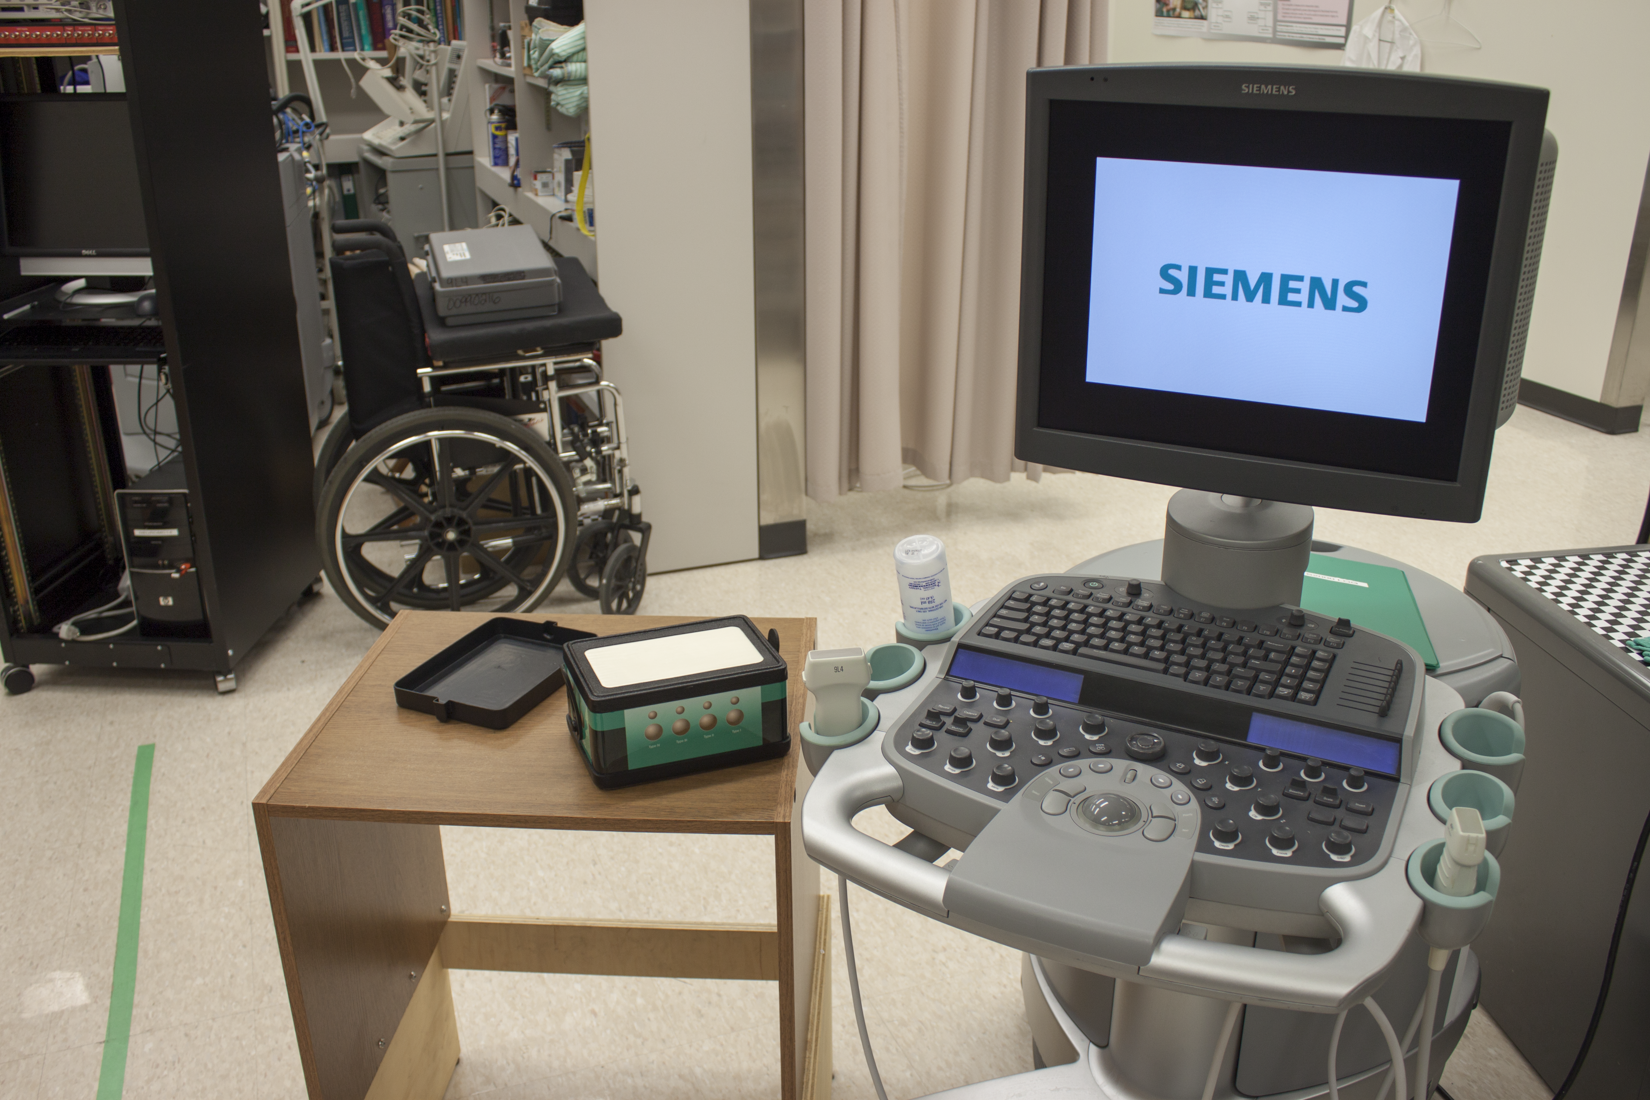
\includegraphics[width=\textwidth]{assets/experimental_setup.png}};

			% the phantom
			\draw[pc1,->,ultra thick] (-0.5, 1) -- (-1,-0.9);
			\draw (-0.5, 1) node[above,text width=1in,align=center,fill=white,rounded corners=3pt,draw=pc1,ultra thick]{\color{black}\footnotesize CIRS Elasticity QA Phantom model 049};

			% the probe
			\draw[pc2,->,ultra thick] (-2, -3.15) -- (0, -1.3);
			\draw (-2, -3.15) node[below,text width=1in,align=center,fill=white,rounded corners=3pt,draw=pc2,ultra thick]{\color{black}\footnotesize 9L4 Transducer};

			% the ultrasound machine
			\draw[pc3,->,ultra thick] (-0.5, 4) -- (2.5, 2.5);
			\draw (-0.5, 4) node[left,text width=1.5in,align=center,fill=white,rounded corners=3pt,draw=pc3,ultra thick]{\color{black}\footnotesize Siemens ACUSON S2000\textsuperscript{\texttrademark}\ portable ultrasound machine};
		\end{tikzpicture}
		\caption[]{Experimental setup showing the ultrasound machine, probe, and phantom model.}
		\label{fig:experimental_photo}
	\end{figure*}

	\section{Quasi-Static Ultrasound Elastography}
		\label{appsec:experimental_quasistatic}
		\begin{enumerate}
			\item Apply a layer of ultrasound gel to the active transducer area
			\item Begin a new ``2D'' imaging sequence on the machine using the ``Breast'' preset
			\item \label{itqs:position_transducer} Position the transducer for the desired lesion
			\begin{enumerate}
				\item Note the planar location of the lesion denoted on the sides of the phantom model
				\item Place the active component on the surface of the phantom model
				\item Align the transducer so as to intersect the lesion's planar location in a perpendicular manner
			\end{enumerate}
			\item Adjust the depth of the image to reach the full domain depth of the phantom model (approximately \SI{7.5}{\cm})
			\item Save the current screen
			\item Manually indent the transducer into the tissue by approximately \SI{0.5}{\cm}
			\item \label{itqs:save_second_image} Save the current screen
			\item Repeat steps \ref{itqs:position_transducer} -- \ref{itqs:save_second_image} until all desired images have been acquired
			\item Export the images to ``USB in PC format''
			\item Import the images into MATLAB\textsuperscript{\textregistered}
			\begin{enumerate}
				\item Crop the images so only the imaged domain is visible
			\end{enumerate}
			\item Process the cropped images using a strain estimation algorithm
		\end{enumerate}

	\section{Acoustic Radiation Force Impulse Imaging}
		\label{appsec:experimental_arfi}
		\begin{enumerate}
			\item Apply a layer of ultrasound gel to the active transducer area
			\item Begin a new ``2D'' imaging sequence on the machine using the ``Breast'' preset
			\item \label{itar:position_transducer} Position the transducer for the desired lesion
			\begin{enumerate}
				\item Note the planar location of the lesion denoted on the sides of the phantom model
				\item Place the active component on the surface of the phantom model
				\item Align the transducer so as to intersect the lesion's planar location in a perpendicular manner
			\end{enumerate}
			\item Adjust the depth of the image to reach the full domain depth of the phantom model (approximately \SI{7.5}{\cm})
			\item Using the ultrasound machine's trackball, select the ``Virtual Touch imaging'' button
			\item Ensure the elastogram colour map is a gradient from black to white
			\item Using the trackball and the ``Next'' button, adjust the position and size of the region of interest in order to fully capture the lesion and surrounding tissue
			\item Press the ``Update'' button and hold the transducer as motionless as possible while the scan completes
			\item Save the current screen
			\item \label{itar:unfreeze} Wait for the cooling process to complete then press the ``Freeze'' button to unfreeze the image
			\item Repeat steps \ref{itar:position_transducer} -- \ref{itar:unfreeze} until all desired images have been acquired
			\item Export the images to ``USB in PC format''
			\item Import the images into MATLAB\textsuperscript{\textregistered}
			\item Calculate the stiffness ratios by comparing the mean brightness of the elastograms inside the lesion to the mean brightness of the elastograms in an identical area located superior to the lesion
		\end{enumerate}

	\section{Shear Wave Speed Quantification}
		\label{appsec:experimental_shear}
		\begin{enumerate}
			\item Apply a layer of ultrasound gel to the active transducer area
			\item Begin a new ``2D'' imaging sequence on the machine using the ``Breast'' preset
			\item \label{itsh:position_transducer} Position the transducer for the desired lesion
			\begin{enumerate}
				\item Note the planar location of the lesion denoted on the sides of the phantom model
				\item Place the active component on the surface of the phantom model
				\item Align the transducer so as to intersect the lesion's planar location in a perpendicular manner
			\end{enumerate}
			\item Adjust the depth of the image to reach the full domain depth of the phantom model (approximately \SI{7.5}{\cm})
			\item Using the ultrasound machine's trackball, select the ``Virtual Touch Quantification imaging'' button
			\item Using the trackball, position the region of interest within the lesionous region
			\item Press the ``Update'' button and hold the transducer as motionless as possible while the scan completes
			\item Record the shear wave speed ($Vs$) of the interrogated region
			\item Wait for the cooling process to complete then press the ``Freeze'' button to unfreeze the image
			\item Using the trackball, position the region of interest outside the lesionous region
			\item Press the ``Update'' button and hold the transducer as motionless as possible while the scan completes
			\item Record the shear wave speed ($Vs$) of the interrogated region
			\item \label{itsh:unfreeze} Wait for the cooling process to complete then press the ``Freeze'' button to unfreeze the image
			\item Repeat steps \ref{itsh:position_transducer} -- \ref{itsh:unfreeze} until all desired lesions have been investigated
		\end{enumerate}
\end{appendices}

\end{document}